%%%%%%%%%%%%%%%%%%%%%%%%%%%%%%%%%%%%%%%%%
% The Legrand Orange Book
% LaTeX Template
% Version 2.2 (30/3/17)
%
% This template has been downloaded from:
% http://www.LaTeXTemplates.com
%
% Original author:
% Mathias Legrand (legrand.mathias@gmail.com) with modifications by:
% Vel (vel@latextemplates.com)
%
% License:
% CC BY-NC-SA 3.0 (http://creativecommons.org/licenses/by-nc-sa/3.0/)
%
% Compiling this template:
% This template uses biber for its bibliography and makeindex for its index.
% When you first open the template, compile it from the command line with the 
% commands below to make sure your LaTeX distribution is configured correctly:
%
% 1) pdflatex main
% 2) makeindex main.idx -s StyleInd.ist
% 3) biber main
% 4) pdflatex main x 2
%
% After this, when you wish to update the bibliography/index use the appropriate
% command above and make sure to compile with pdflatex several times 
% afterwards to propagate your changes to the document.
%
% This template also uses a number of packages which may need to be
% updated to the newest versions for the template to compile. It is strongly
% recommended you update your LaTeX distribution if you have any
% compilation errors.
%
% Important note:
% Chapter heading images should have a 2:1 width:height ratio,
% e.g. 920px width and 460px height.
%
%%%%%%%%%%%%%%%%%%%%%%%%%%%%%%%%%%%%%%%%%

%----------------------------------------------------------------------------------------
%	PACKAGES AND OTHER DOCUMENT CONFIGURATIONS
%----------------------------------------------------------------------------------------

\documentclass[11pt,fleqn]{book} % Default font size and left-justified equations



%----------------------------------------------------------------------------------------

%%%%%%%%%%%%%%%%%%%%%%%%%%%%%%%%%%%%%%%%%
% The Legrand Orange Book
% Structural Definitions File
% Version 2.0 (9/2/15)
%
% Original author:
% Mathias Legrand (legrand.mathias@gmail.com) with modifications by:
% Vel (vel@latextemplates.com)
% 
% This file has been downloaded from:
% http://www.LaTeXTemplates.com
%
% License:
% CC BY-NC-SA 3.0 (http://creativecommons.org/licenses/by-nc-sa/3.0/)
%
%%%%%%%%%%%%%%%%%%%%%%%%%%%%%%%%%%%%%%%%%

%----------------------------------------------------------------------------------------
%	VARIOUS REQUIRED PACKAGES AND CONFIGURATIONS
%----------------------------------------------------------------------------------------

\usepackage[top=3cm,bottom=3cm,left=3cm,right=3cm,headsep=10pt,a4paper]{geometry} % Page margins

\usepackage{graphicx} % Required for including pictures
\graphicspath{{Pictures/}} % Specifies the directory where pictures are stored

\usepackage{lipsum} % Inserts dummy text

\usepackage{tikz} % Required for drawing custom shapes

\usepackage[english]{babel} % English language/hyphenation

\usepackage{enumitem} % Customize lists
\setlist{nolistsep} % Reduce spacing between bullet points and numbered lists

\usepackage{booktabs} % Required for nicer horizontal rules in tables

\usepackage{xcolor} % Required for specifying colors by name
\definecolor{ocre}{RGB}{243,102,25} % Define the orange color used for highlighting throughout the book

%----------------------------------------------------------------------------------------
%	FONTS
%----------------------------------------------------------------------------------------

\usepackage{avant} % Use the Avantgarde font for headings
%\usepackage{times} % Use the Times font for headings
\usepackage{mathptmx} % Use the Adobe Times Roman as the default text font together with math symbols from the Sym­bol, Chancery and Com­puter Modern fonts

\usepackage{microtype} % Slightly tweak font spacing for aesthetics
\usepackage[utf8]{inputenc} % Required for including letters with accents
\usepackage[T1]{fontenc} % Use 8-bit encoding that has 256 glyphs

%----------------------------------------------------------------------------------------
%	BIBLIOGRAPHY AND INDEX
%----------------------------------------------------------------------------------------

\usepackage[style=alphabetic,citestyle=numeric,sorting=nyt,sortcites=true,autopunct=true,babel=hyphen,hyperref=true,abbreviate=false,backref=true,backend=biber]{biblatex}
\addbibresource{bibliography.bib} % BibTeX bibliography file
\defbibheading{bibempty}{}

\usepackage{calc} % For simpler calculation - used for spacing the index letter headings correctly
\usepackage{makeidx} % Required to make an index
\makeindex % Tells LaTeX to create the files required for indexing

%----------------------------------------------------------------------------------------
%	MAIN TABLE OF CONTENTS
%----------------------------------------------------------------------------------------

\usepackage{titletoc} % Required for manipulating the table of contents

\contentsmargin{0cm} % Removes the default margin

% Part text styling
\titlecontents{part}[0cm]
{\addvspace{20pt}\centering\large\bfseries}
{}
{}
{}

% Chapter text styling
\titlecontents{chapter}[1.25cm] % Indentation
{\addvspace{12pt}\large\sffamily\bfseries} % Spacing and font options for chapters
{\color{ocre!60}\contentslabel[\Large\thecontentslabel]{1.25cm}\color{ocre}} % Chapter number
{\color{ocre}}  
{\color{ocre!60}\normalsize\;\titlerule*[.5pc]{.}\;\thecontentspage} % Page number

% Section text styling
\titlecontents{section}[1.25cm] % Indentation
{\addvspace{3pt}\sffamily\bfseries} % Spacing and font options for sections
{\contentslabel[\thecontentslabel]{1.25cm}} % Section number
{}
{\hfill\color{black}\thecontentspage} % Page number
[]

% Subsection text styling
\titlecontents{subsection}[1.25cm] % Indentation
{\addvspace{1pt}\sffamily\small} % Spacing and font options for subsections
{\contentslabel[\thecontentslabel]{1.25cm}} % Subsection number
{}
{\ \titlerule*[.5pc]{.}\;\thecontentspage} % Page number
[]

% List of figures
\titlecontents{figure}[0em]
{\addvspace{-5pt}\sffamily}
{\thecontentslabel\hspace*{1em}}
{}
{\ \titlerule*[.5pc]{.}\;\thecontentspage}
[]

% List of tables
\titlecontents{table}[0em]
{\addvspace{-5pt}\sffamily}
{\thecontentslabel\hspace*{1em}}
{}
{\ \titlerule*[.5pc]{.}\;\thecontentspage}
[]

%----------------------------------------------------------------------------------------
%	MINI TABLE OF CONTENTS IN PART HEADS
%----------------------------------------------------------------------------------------

% Chapter text styling
\titlecontents{lchapter}[0em] % Indenting
{\addvspace{15pt}\large\sffamily\bfseries} % Spacing and font options for chapters
{\color{ocre}\contentslabel[\Large\thecontentslabel]{1.25cm}\color{ocre}} % Chapter number
{}  
{\color{ocre}\normalsize\sffamily\bfseries\;\titlerule*[.5pc]{.}\;\thecontentspage} % Page number

% Section text styling
\titlecontents{lsection}[0em] % Indenting
{\sffamily\small} % Spacing and font options for sections
{\contentslabel[\thecontentslabel]{1.25cm}} % Section number
{}
{}

% Subsection text styling
\titlecontents{lsubsection}[.5em] % Indentation
{\normalfont\footnotesize\sffamily} % Font settings
{}
{}
{}

%----------------------------------------------------------------------------------------
%	PAGE HEADERS
%----------------------------------------------------------------------------------------

\usepackage{fancyhdr} % Required for header and footer configuration

\pagestyle{fancy}
\renewcommand{\chaptermark}[1]{\markboth{\sffamily\normalsize\bfseries\chaptername\ \thechapter.\ #1}{}} % Chapter text font settings
\renewcommand{\sectionmark}[1]{\markright{\sffamily\normalsize\thesection\hspace{5pt}#1}{}} % Section text font settings
\fancyhf{} \fancyhead[LE,RO]{\sffamily\normalsize\thepage} % Font setting for the page number in the header
\fancyhead[LO]{\rightmark} % Print the nearest section name on the left side of odd pages
\fancyhead[RE]{\leftmark} % Print the current chapter name on the right side of even pages
\renewcommand{\headrulewidth}{0.5pt} % Width of the rule under the header
\addtolength{\headheight}{2.5pt} % Increase the spacing around the header slightly
\renewcommand{\footrulewidth}{0pt} % Removes the rule in the footer
\fancypagestyle{plain}{\fancyhead{}\renewcommand{\headrulewidth}{0pt}} % Style for when a plain pagestyle is specified

% Removes the header from odd empty pages at the end of chapters
\makeatletter
\renewcommand{\cleardoublepage}{
\clearpage\ifodd\c@page\else
\hbox{}
\vspace*{\fill}
\thispagestyle{empty}
\newpage
\fi}

%----------------------------------------------------------------------------------------
%	THEOREM STYLES
%----------------------------------------------------------------------------------------

\usepackage{amsmath,amsfonts,amssymb,amsthm} % For math equations, theorems, symbols, etc

\newcommand{\intoo}[2]{\mathopen{]}#1\,;#2\mathclose{[}}
\newcommand{\ud}{\mathop{\mathrm{{}d}}\mathopen{}}
\newcommand{\intff}[2]{\mathopen{[}#1\,;#2\mathclose{]}}
\newtheorem{notation}{Notation}[chapter]

% Boxed/framed environments
\newtheoremstyle{ocrenumbox}% % Theorem style name
{0pt}% Space above
{0pt}% Space below
{\normalfont}% % Body font
{}% Indent amount
{\small\bf\sffamily\color{ocre}}% % Theorem head font
{\;}% Punctuation after theorem head
{0.25em}% Space after theorem head
{\small\sffamily\color{ocre}\thmname{#1}\nobreakspace\thmnumber{\@ifnotempty{#1}{}\@upn{#2}}% Theorem text (e.g. Theorem 2.1)
\thmnote{\nobreakspace\the\thm@notefont\sffamily\bfseries\color{black}---\nobreakspace#3.}} % Optional theorem note
\renewcommand{\qedsymbol}{$\blacksquare$}% Optional qed square

\newtheoremstyle{blacknumex}% Theorem style name
{5pt}% Space above
{5pt}% Space below
{\normalfont}% Body font
{} % Indent amount
{\small\bf\sffamily}% Theorem head font
{\;}% Punctuation after theorem head
{0.25em}% Space after theorem head
{\small\sffamily{\tiny\ensuremath{\blacksquare}}\nobreakspace\thmname{#1}\nobreakspace\thmnumber{\@ifnotempty{#1}{}\@upn{#2}}% Theorem text (e.g. Theorem 2.1)
\thmnote{\nobreakspace\the\thm@notefont\sffamily\bfseries---\nobreakspace#3.}}% Optional theorem note

\newtheoremstyle{blacknumbox} % Theorem style name
{0pt}% Space above
{0pt}% Space below
{\normalfont}% Body font
{}% Indent amount
{\small\bf\sffamily}% Theorem head font
{\;}% Punctuation after theorem head
{0.25em}% Space after theorem head
{\small\sffamily\thmname{#1}\nobreakspace\thmnumber{\@ifnotempty{#1}{}\@upn{#2}}% Theorem text (e.g. Theorem 2.1)
\thmnote{\nobreakspace\the\thm@notefont\sffamily\bfseries---\nobreakspace#3.}}% Optional theorem note

% Non-boxed/non-framed environments
\newtheoremstyle{ocrenum}% % Theorem style name
{5pt}% Space above
{5pt}% Space below
{\normalfont}% % Body font
{}% Indent amount
{\small\bf\sffamily\color{ocre}}% % Theorem head font
{\;}% Punctuation after theorem head
{0.25em}% Space after theorem head
{\small\sffamily\color{ocre}\thmname{#1}\nobreakspace\thmnumber{\@ifnotempty{#1}{}\@upn{#2}}% Theorem text (e.g. Theorem 2.1)
\thmnote{\nobreakspace\the\thm@notefont\sffamily\bfseries\color{black}---\nobreakspace#3.}} % Optional theorem note
\renewcommand{\qedsymbol}{$\blacksquare$}% Optional qed square
\makeatother

% Defines the theorem text style for each type of theorem to one of the three styles above
\newcounter{dummy} 
\numberwithin{dummy}{section}
\theoremstyle{ocrenumbox}
\newtheorem{theoremeT}[dummy]{Theorem}
\newtheorem{problem}{Problem}[chapter]
\newtheorem{exerciseT}{Exercise}[chapter]
\theoremstyle{blacknumex}
\newtheorem{exampleT}{Example}[chapter]
\theoremstyle{blacknumbox}
\newtheorem{vocabulary}{Vocabulary}[chapter]
\newtheorem{definitionT}{Definition}[section]
\newtheorem{corollaryT}[dummy]{Corollary}
\theoremstyle{ocrenum}
\newtheorem{proposition}[dummy]{Proposition}

%----------------------------------------------------------------------------------------
%	DEFINITION OF COLORED BOXES
%----------------------------------------------------------------------------------------

\RequirePackage[framemethod=default]{mdframed} % Required for creating the theorem, definition, exercise and corollary boxes

% Theorem box
\newmdenv[skipabove=7pt,
skipbelow=7pt,
backgroundcolor=black!5,
linecolor=ocre,
innerleftmargin=5pt,
innerrightmargin=5pt,
innertopmargin=5pt,
leftmargin=0cm,
rightmargin=0cm,
innerbottommargin=5pt]{tBox}

% Exercise box	  
\newmdenv[skipabove=7pt,
skipbelow=7pt,
rightline=false,
leftline=true,
topline=false,
bottomline=false,
backgroundcolor=ocre!10,
linecolor=ocre,
innerleftmargin=5pt,
innerrightmargin=5pt,
innertopmargin=5pt,
innerbottommargin=5pt,
leftmargin=0cm,
rightmargin=0cm,
linewidth=4pt]{eBox}	

% Definition box
\newmdenv[skipabove=7pt,
skipbelow=7pt,
rightline=false,
leftline=true,
topline=false,
bottomline=false,
linecolor=ocre,
innerleftmargin=5pt,
innerrightmargin=5pt,
innertopmargin=0pt,
leftmargin=0cm,
rightmargin=0cm,
linewidth=4pt,
innerbottommargin=0pt]{dBox}	

% Corollary box
\newmdenv[skipabove=7pt,
skipbelow=7pt,
rightline=false,
leftline=true,
topline=false,
bottomline=false,
linecolor=gray,
backgroundcolor=black!5,
innerleftmargin=5pt,
innerrightmargin=5pt,
innertopmargin=5pt,
leftmargin=0cm,
rightmargin=0cm,
linewidth=4pt,
innerbottommargin=5pt]{cBox}

% Creates an environment for each type of theorem and assigns it a theorem text style from the "Theorem Styles" section above and a colored box from above
\newenvironment{theorem}{\begin{tBox}\begin{theoremeT}}{\end{theoremeT}\end{tBox}}
\newenvironment{exercise}{\begin{eBox}\begin{exerciseT}}{\hfill{\color{ocre}\tiny\ensuremath{\blacksquare}}\end{exerciseT}\end{eBox}}				  
\newenvironment{definition}{\begin{dBox}\begin{definitionT}}{\end{definitionT}\end{dBox}}	
\newenvironment{example}{\begin{exampleT}}{\hfill{\tiny\ensuremath{\blacksquare}}\end{exampleT}}		
\newenvironment{corollary}{\begin{cBox}\begin{corollaryT}}{\end{corollaryT}\end{cBox}}	

%----------------------------------------------------------------------------------------
%	REMARK ENVIRONMENT
%----------------------------------------------------------------------------------------

\newenvironment{remark}{\par\vspace{10pt}\small % Vertical white space above the remark and smaller font size
\begin{list}{}{
\leftmargin=35pt % Indentation on the left
\rightmargin=25pt}\item\ignorespaces % Indentation on the right
\makebox[-2.5pt]{\begin{tikzpicture}[overlay]
\node[draw=ocre!60,line width=1pt,circle,fill=ocre!25,font=\sffamily\bfseries,inner sep=2pt,outer sep=0pt] at (-15pt,0pt){\textcolor{ocre}{R}};\end{tikzpicture}} % Orange R in a circle
\advance\baselineskip -1pt}{\end{list}\vskip5pt} % Tighter line spacing and white space after remark

%----------------------------------------------------------------------------------------
%	SECTION NUMBERING IN THE MARGIN
%----------------------------------------------------------------------------------------

\makeatletter
\renewcommand{\@seccntformat}[1]{\llap{\textcolor{ocre}{\csname the#1\endcsname}\hspace{1em}}}                    
\renewcommand{\section}{\@startsection{section}{1}{\z@}
{-4ex \@plus -1ex \@minus -.4ex}
{1ex \@plus.2ex }
{\normalfont\large\sffamily\bfseries}}
\renewcommand{\subsection}{\@startsection {subsection}{2}{\z@}
{-3ex \@plus -0.1ex \@minus -.4ex}
{0.5ex \@plus.2ex }
{\normalfont\sffamily\bfseries}}
\renewcommand{\subsubsection}{\@startsection {subsubsection}{3}{\z@}
{-2ex \@plus -0.1ex \@minus -.2ex}
{.2ex \@plus.2ex }
{\normalfont\small\sffamily\bfseries}}                        
\renewcommand\paragraph{\@startsection{paragraph}{4}{\z@}
{-2ex \@plus-.2ex \@minus .2ex}
{.1ex}
{\normalfont\small\sffamily\bfseries}}

%----------------------------------------------------------------------------------------
%	PART HEADINGS
%----------------------------------------------------------------------------------------

% numbered part in the table of contents
\newcommand{\@mypartnumtocformat}[2]{%
\setlength\fboxsep{0pt}%
\noindent\colorbox{ocre!20}{\strut\parbox[c][.7cm]{\ecart}{\color{ocre!70}\Large\sffamily\bfseries\centering#1}}\hskip\esp\colorbox{ocre!40}{\strut\parbox[c][.7cm]{\linewidth-\ecart-\esp}{\Large\sffamily\centering#2}}}%
%%%%%%%%%%%%%%%%%%%%%%%%%%%%%%%%%%
% unnumbered part in the table of contents
\newcommand{\@myparttocformat}[1]{%
\setlength\fboxsep{0pt}%
\noindent\colorbox{ocre!40}{\strut\parbox[c][.7cm]{\linewidth}{\Large\sffamily\centering#1}}}%
%%%%%%%%%%%%%%%%%%%%%%%%%%%%%%%%%%
\newlength\esp
\setlength\esp{4pt}
\newlength\ecart
\setlength\ecart{1.2cm-\esp}
\newcommand{\thepartimage}{}%
\newcommand{\partimage}[1]{\renewcommand{\thepartimage}{#1}}%
\def\@part[#1]#2{%
\ifnum \c@secnumdepth >-2\relax%
\refstepcounter{part}%
\addcontentsline{toc}{part}{\texorpdfstring{\protect\@mypartnumtocformat{\thepart}{#1}}{\partname~\thepart\ ---\ #1}}
\else%
\addcontentsline{toc}{part}{\texorpdfstring{\protect\@myparttocformat{#1}}{#1}}%
\fi%
\startcontents%
\markboth{}{}%
{\thispagestyle{empty}%
\begin{tikzpicture}[remember picture,overlay]%
\node at (current page.north west){\begin{tikzpicture}[remember picture,overlay]%	
\fill[ocre!20](0cm,0cm) rectangle (\paperwidth,-\paperheight);
\node[anchor=north] at (4cm,-3.25cm){\color{ocre!40}\fontsize{220}{100}\sffamily\bfseries\thepart}; 
\node[anchor=south east] at (\paperwidth-1cm,-\paperheight+1cm){\parbox[t][][t]{8.5cm}{
\printcontents{l}{0}{\setcounter{tocdepth}{1}}%
}};
\node[anchor=north east] at (\paperwidth-1.5cm,-3.25cm){\parbox[t][][t]{15cm}{\strut\raggedleft\color{white}\fontsize{30}{30}\sffamily\bfseries#2}};
\end{tikzpicture}};
\end{tikzpicture}}%
\@endpart}
\def\@spart#1{%
\startcontents%
\phantomsection
{\thispagestyle{empty}%
\begin{tikzpicture}[remember picture,overlay]%
\node at (current page.north west){\begin{tikzpicture}[remember picture,overlay]%	
\fill[ocre!20](0cm,0cm) rectangle (\paperwidth,-\paperheight);
\node[anchor=north east] at (\paperwidth-1.5cm,-3.25cm){\parbox[t][][t]{15cm}{\strut\raggedleft\color{white}\fontsize{30}{30}\sffamily\bfseries#1}};
\end{tikzpicture}};
\end{tikzpicture}}
\addcontentsline{toc}{part}{\texorpdfstring{%
\setlength\fboxsep{0pt}%
\noindent\protect\colorbox{ocre!40}{\strut\protect\parbox[c][.7cm]{\linewidth}{\Large\sffamily\protect\centering #1\quad\mbox{}}}}{#1}}%
\@endpart}
\def\@endpart{\vfil\newpage
\if@twoside
\if@openright
\null
\thispagestyle{empty}%
\newpage
\fi
\fi
\if@tempswa
\twocolumn
\fi}

%----------------------------------------------------------------------------------------
%	CHAPTER HEADINGS
%----------------------------------------------------------------------------------------

% A switch to conditionally include a picture, implemented by  Christian Hupfer
\newif\ifusechapterimage
\usechapterimagetrue
\newcommand{\thechapterimage}{}%
\newcommand{\chapterimage}[1]{\ifusechapterimage\renewcommand{\thechapterimage}{#1}\fi}%
\newcommand{\autodot}{.}
\def\@makechapterhead#1{%
{\parindent \z@ \raggedright \normalfont
\ifnum \c@secnumdepth >\m@ne
\if@mainmatter
\begin{tikzpicture}[remember picture,overlay]
\node at (current page.north west)
{\begin{tikzpicture}[remember picture,overlay]
\node[anchor=north west,inner sep=0pt] at (0,0) {\ifusechapterimage\includegraphics[width=\paperwidth]{\thechapterimage}\fi};
\draw[anchor=west] (\Gm@lmargin,-9cm) node [line width=2pt,rounded corners=15pt,draw=ocre,fill=white,fill opacity=0.5,inner sep=15pt]{\strut\makebox[22cm]{}};
\draw[anchor=west] (\Gm@lmargin+.3cm,-9cm) node {\huge\sffamily\bfseries\color{black}\thechapter\autodot~#1\strut};
\end{tikzpicture}};
\end{tikzpicture}
\else
\begin{tikzpicture}[remember picture,overlay]
\node at (current page.north west)
{\begin{tikzpicture}[remember picture,overlay]
\node[anchor=north west,inner sep=0pt] at (0,0) {\ifusechapterimage\includegraphics[width=\paperwidth]{\thechapterimage}\fi};
\draw[anchor=west] (\Gm@lmargin,-9cm) node [line width=2pt,rounded corners=15pt,draw=ocre,fill=white,fill opacity=0.5,inner sep=15pt]{\strut\makebox[22cm]{}};
\draw[anchor=west] (\Gm@lmargin+.3cm,-9cm) node {\huge\sffamily\bfseries\color{black}#1\strut};
\end{tikzpicture}};
\end{tikzpicture}
\fi\fi\par\vspace*{270\p@}}}

%-------------------------------------------

\def\@makeschapterhead#1{%
\begin{tikzpicture}[remember picture,overlay]
\node at (current page.north west)
{\begin{tikzpicture}[remember picture,overlay]
\node[anchor=north west,inner sep=0pt] at (0,0) {\ifusechapterimage\includegraphics[width=\paperwidth]{\thechapterimage}\fi};
\draw[anchor=west] (\Gm@lmargin,-9cm) node [line width=2pt,rounded corners=15pt,draw=ocre,fill=white,fill opacity=0.5,inner sep=15pt]{\strut\makebox[22cm]{}};
\draw[anchor=west] (\Gm@lmargin+.3cm,-9cm) node {\huge\sffamily\bfseries\color{black}#1\strut};
\end{tikzpicture}};
\end{tikzpicture}
\par\vspace*{270\p@}}
\makeatother

%----------------------------------------------------------------------------------------
%	HYPERLINKS IN THE DOCUMENTS
%----------------------------------------------------------------------------------------

\usepackage{hyperref}
\hypersetup{hidelinks,backref=true,pagebackref=true,hyperindex=true,colorlinks=false,breaklinks=true,urlcolor= ocre,bookmarks=true,bookmarksopen=false,pdftitle={Title},pdfauthor={Author}}
\usepackage{bookmark}
\bookmarksetup{
open,
numbered,
addtohook={%
\ifnum\bookmarkget{level}=0 % chapter
\bookmarksetup{bold}%
\fi
\ifnum\bookmarkget{level}=-1 % part
\bookmarksetup{color=ocre,bold}%
\fi
}
}
 % Insert the commands.tex file which contains the majority of the structure behind the template

\begin{document}

%----------------------------------------------------------------------------------------
%	TITLE PAGE
%----------------------------------------------------------------------------------------

\begingroup
\thispagestyle{empty}
\begin{tikzpicture}[remember picture,overlay]
\node[inner sep=0pt] (background) at (current page.center) {
\includegraphics[width=\paperwidth]{background}};
\draw (current page.center) node [fill=ocre!30!white,fill opacity=0.6,text opacity=1,inner sep=1cm]{\Huge\centering\bfseries\sffamily\parbox[c][][t]{\paperwidth}{\centering The Search for a Title\\[15pt] % Book title
{\Large A Profound Subtitle}\\[20pt] % Subtitle
{\huge Dr. John Smith}}}; % Author name
\end{tikzpicture}
\vfill
\endgroup

%----------------------------------------------------------------------------------------
%	COPYRIGHT PAGE
%----------------------------------------------------------------------------------------

\newpage
~\vfill
\thispagestyle{empty}

\noindent Copyright \copyright\ 2013 John Smith\\ % Copyright notice

\noindent \textsc{Published by Publisher}\\ % Publisher

\noindent \textsc{book-website.com}\\ % URL

\noindent Licensed under the Creative Commons Attribution-NonCommercial 3.0 Unported License (the ``License''). You may not use this file except in compliance with the License. You may obtain a copy of the License at \url{http://creativecommons.org/licenses/by-nc/3.0}. Unless required by applicable law or agreed to in writing, software distributed under the License is distributed on an \textsc{``as is'' basis, without warranties or conditions of any kind}, either express or implied. See the License for the specific language governing permissions and limitations under the License.\\ % License information

\noindent \textit{First printing, March 2013} % Printing/edition date

%----------------------------------------------------------------------------------------
%	TABLE OF CONTENTS
%----------------------------------------------------------------------------------------

%\usechapterimagefalse % If you don't want to include a chapter image, use this to toggle images off - it can be enabled later with \usechapterimagetrue

\chapterimage{chapter_head_1.pdf} % Table of contents heading image

\pagestyle{empty} % No headers

\tableofcontents % Print the table of contents itself

\cleardoublepage % Forces the first chapter to start on an odd page so it's on the right

\pagestyle{fancy} % Print headers again

%----------------------------------------------------------------------------------------
%	PART
%----------------------------------------------------------------------------------------

\part{Part One}

%----------------------------------------------------------------------------------------
%	CHAPTER 1
%----------------------------------------------------------------------------------------

\chapterimage{chapter_head_2.pdf} % Chapter heading image

\chapter{Persamaan dan Pertidaksamaan Linear Satu Variabel yang Memuat Nilai Mutlak}

\section{Persamaan dan pertidaksamaan linear satu variabel yang memuat nilai mutlak}\index{Persamaan dan pertidaksamaan linear satu variabel yang memuat nilai mutlak}

\noindent \textbf{}


\subsection{ Pendahuluan}


\paragraph{ Kompetensi Dasar}


\subparagraph{ Mengintepretasi persamaan dan pertidaksamaan nilai mutlak dari bentuk linear satu variabel dengan persamaan dan pertidaksamaan linear Aljabar lainnya.}


\subparagraph{ Menyelesaikan masalah yang berkaitan dengan persamaan dan pertidaksamaan nilai mutlak dari bentuk linear satu variable.}


\paragraph{ Indikator}

\begin{enumerate}
\item \textbf{ }Menjelaskan konsep nilai mutlak\textbf{}

\item \textbf{ }Menyelesaikan persamaan nilai mutlak\textbf{}

\item \textbf{ }Menyelesaikan pertidaksamaan nilai mutlak satu variable\textbf{}

\item \textbf{ }Menyelesaikan masalah yang berkaitan dengan persamaan satu variable yang memuat nilai mutlak\textbf{}
\end{enumerate}


\paragraph{ Materi Pokok}

\noindent Persamaan dan pertidaksamaan nilai mutlak linear satu variable
\noindent
\noindent
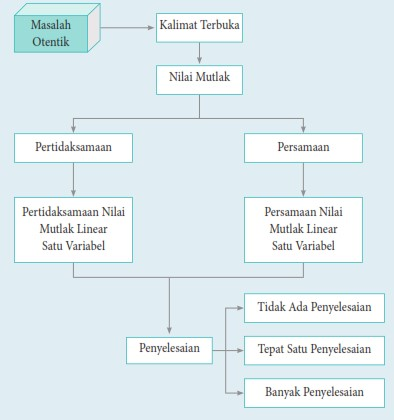
\includegraphics[width=3in, height=3in, keepaspectratio=false]{t1}

\noindent 


\subsection{ Uraian Materi}


\paragraph{ Kalimat Terbuka, Variabel, dan Konstanta}

Kalimat terbuka adalah kalimat yang belum dapat diketahui nilai kebenarannya.

\noindent Variable (peubah) adalah lambang (symbol) pada kalimat terbuka yang dapat diganti oleh sembarang anggota himpunan yang telah ditentukan

\noindent Konstanta adalah lambang yang menyatakan suatu bilangan tertentu

\noindent Pada kalimat berikut 

\noindent x + 5 = 12

Belum dapat mengatakan kalimat itu benar atau salah, sebab nilai (x) belum diketahui. Bila lambang (x) diganti dengan lambang bilangan cacah, barulah itu dapat dikatakan kalimat itu benar atau salah. Jika (x) diganti dengan ``3'' , kalimat itu bernilai salah ; tetapi bila (x) diganti dengan 7 , kalimat itu bernilai benar. Lambang (x) dapat pula diganti menggunaan huruf-huruf kecil dalam abjad lainnya, yaitu ; a, b,c,{\dots} x,y,z dari bentuk diatas

\noindent x+5 +12 ~~~~~~~~~ (kalimat terbuka)

\noindent 3+ 5 = 12 ~~~~~~~ ~(kalimat Salah )

\noindent 7+5 = 12 ~~~~~~~~ (kalimat benar)

\noindent Huruf x pada x + 5 = 12 disebut variable (peubah), sedangkan 5 dan 12 disebut konstanta

\noindent Contoh :

\noindent 

\begin{tabular}{|p{2.1in}|p{0.7in}|p{1.1in}|} \hline 
\textbf{Kalimat Terbuka} & \textbf{Peubah} & \textbf{Konstanta} \\ \hline 
x + 13 + 17 & x & 13 dan 17 \\ \hline 
7 -- y = 12 & y & 7 dan 12 \\ \hline 
4z -- 1 = 11 & z & -1 dan 11 \\ \hline 
\end{tabular}

Catatan :

\noindent Kalimat terbuka adalah kalimat yang mengandung satu atau lebih variabel dan belum diketahui nilai kebenarannya, contoh :

\noindent x + 2 =5

\noindent 


\paragraph{ Konsep Nilai Mutlak}

\includegraphics*[width=3.10in, height=0.57in, keepaspectratio=false]{t2} Nilai mutlak suatu bilangan dapat diartikan jarak antara bilangan tersebut dari titik nol(0). 

Dengan demikian jarak selalu bernilai positif.



\noindent \includegraphics*[width=5.24in, height=0.98in, keepaspectratio=false]{t3}

\noindent Jarak angka 6 dari titik 0 adalah 6

\noindent Jarak angka -6 dari titik 0 adalah 6~

\noindent jarak angka -7 dari titik 0 adalah 7

\noindent Jarak angka 5 dari titik 0 adalah 5.

\noindent 

\noindent Dari penjelesan di atas memang tampak bahwa nilai mutlak suatu bilangan selalu bernilai positif.

\noindent \includegraphics*[width=1.65in, height=0.43in, keepaspectratio=false]{t4}  Nilai mutlak dapat didefinisikan dengan Misalkan x bilangan real, didefinisikan

\noindent 

\noindent Nilai mutlak juga dapat didefinisikan dengan 

\noindent \textit{"Apabila x adalah sebuah bentuk aljabar, sedangkan n merupakan bilangan real positif, maka {\textbar}x{\textbar} = n dapat diimplikasikan menjadi x = n atau x = -n". }

\noindent \includegraphics*[width=2.04in, height=0.56in, keepaspectratio=false]{t5}Berkaitan dengan menentukan nilai mutlak suatu bilangan, maka muncullah tanda mutlak. Tanda mutlak disimbolkan dengan~ garis 2 ditepi suatu bilangan atau bentuk aljabar.

\noindent 

\noindent Definisi di atas dapat diungkapkan dengan kalimat sehari-hari seperti berikut ini. Nilai mutlak suatu bilangan positif atau nol adalah bilangan itu sendiri, sedangkan nilai mutlak dari suatu bilangan negatif adalah lawan dari bilangan negatif itu. Dengan demikian, dapat dikatakan bahwa:

\noindent \includegraphics*[width=4.47in, height=1.26in, keepaspectratio=false]{t6}

\noindent Tabel 1.1 Nilai Mutlak

\noindent \includegraphics*[width=5.15in, height=1.52in, keepaspectratio=false]{t7}

\noindent 

 Berdasarkan kedua cerita dan tabel di atas, dapatkah kamu menarik suatu kesimpulan tentang pengertian nilai mutlak? Jika x adalah variabel pengganti sebarang bilangan real, dapatkah kamu menentukan nilai mutlak dari x tersebut?

  Perhatikan bahwa x anggota himpunan bilangan real (ditulis x$\mathrm{\in }$R). Berdasarkan tabel, kita melihat bahwa nilai mutlak dari x akan bernilai positif atau nol (non negatif). Secara geometris, nilai mutlak suatu bilangan adalah jarak antara bilangan itu dengan nol pada garis bilangan real. Dengan demikian, tidak mungkin nilai mutlak suatu bilangan bernilai negatif, tetapi mungkin saja bernilai nol. 

 Ada beberapa contoh percobaan perpindahan posisi pada garis bilangan, yaitu sebagai berikut:

  \includegraphics*[width=3.30in, height=2.37in, keepaspectratio=false]{t8}

\noindent Catatan: 

\noindent  Garis bilangan digunakan sebagai media untuk menunjukkan nilai mutlak. 

\noindent  Tanda panah digunakan untuk menentukan besar nilai mutlak, dimana arah ke kiri menandakan nilai mutlak dari bilangan negatif, dan begitu juga sebaliknya. Arah ke kanan menandakan nilai mutlak dari bilangan positif. 

\noindent  Besar nilai mutlak dilihat dari panjang tanda panah dan dihitung dari bilangan nol.

\noindent 

\noindent Penjelasan 

\noindent \textbf{Garis bilangan 1}: Tanda panah bergerak ke arah kanan berawal dari bilangan 0 menuju bilangan 3, dan besar langkah yang dilalui tanda panah adalah 3. Hal ini berarti nilai {\textbar}3{\textbar} = 3 atau berjarak 3 satuan dari bilangan 0. 

\noindent \textbf{Garis bilangan 5}: Tanda panah bergerak ke arah kiri berawal dari bilangan 0 menuju bilangan -3, dan besar langkah yang dilalui tanda panah adalah 3. Hal ini berarti bahwa nilai {\textbar}-3{\textbar} = 3 atau berjarak 3 satuan dari bilangan 0.

  Dari kedua penjelasan di atas, dapat dituliskan konsep nilai mutlak, sebagai berikut.

\noindent 

   \includegraphics*[width=5.08in, height=1.24in, keepaspectratio=false]{t9}

\noindent 

  Definisi di atas dapat diungkapkan dengan kalimat sehari-hari seperti berikut ini. Nilai mutlak suatu bilangan positif atau nol adalah bilangan itu sendiri, sedangkan nilai mutlak dari suatu bilangan negatif adalah lawan dari bilangan negatif itu. Dengan demikian, dapat dikatakan bahwa:

\noindent  a) 11 = 22 , karena 1 2 $>$0 (1 2 adalah bilangan positif). 

\noindent b) {\textbar}5{\textbar} = 5, karena 5 $>$ 0 (5 adalah bilangan positif).

\noindent  c) {\textbar}-3{\textbar} = -(-3) = 3, karena -3 $<$ 0 (-3 adalah bilangan negatif).


\paragraph{ Persamaan Nilai Mutlak Linear Satu Variabel}

Nilai mutlak dari suatu bilangan \textit{x} dapat diartikan sebagai jarak bilangan tersebut terhadap titik 0 pada garis bilangan, dengan tidak memperhatikan arahnya. Ini berarti {\textbar}\textit{x}{\textbar} = 5 memiliki dua selesaian, karena terdapat dua bilangan yang jaraknya terhadap 0 adalah 5: \textit{x} = --5 dan \textit{x} = 5 (perhatikan gambar berikut).

\noindent \includegraphics*[width=5.01in, height=1.25in, keepaspectratio=false]{t10}

Himpuana Penyelesaian (HP) adalah himpunan dari penyelesaian-penyelesaian suatu persamaan .

\noindent Ada dua cara untuk menentukan penyelesaian dan himpunan penyelesaian dari suatu persamaan linier satu variable , yaitu :

\begin{enumerate}
\item  \textbf{Subtitusi }
\end{enumerate}

\noindent Selesaikan persamaan 3x-1=14; jika x Merupakan anggota himpunan P = ( 3,4,5,6) !

\noindent Jawab :

\noindent 3x-1+14 x ~? P = (3,4,5,6)

\noindent Cara subtitusi :

\noindent 3x-1= 14;~ jika x = 3 = maka 3\eqref{GrindEQ__3_} -- 1 = 8 (salah)

\noindent 3x-1= 14;~ jika x = 4 = maka 3\eqref{GrindEQ__4_} -- 1 = 11 (salah)

\noindent 3x-1= 14;~ jika x = 5 = maka 3\eqref{GrindEQ__5_} -- 1 = 14 (benar)

\noindent 3x-1= 14;~ jika x = 6 = maka 3\eqref{GrindEQ__6_} -- 1 = 17 (salah)

\noindent Jadi , penyelesaian dari 3x-1+14 adalah 5

\noindent 

\begin{enumerate}
\item  \textbf{Mencari persamaan-persamaan yang ekuivalen}
\end{enumerate}

Mencari persamaan-persamaan yang ekuivalen

\noindent 

\begin{tabular}{|p{0.4in}|p{0.7in}|p{1.3in}|p{1.3in}|} \hline 
 & Persamaan & Operasi Hitung & Hasil \\ \hline 
A\newline \newline b.\newline \newline c. & 3x-1=14 (i) & Kedua ruas ditambah 1 & 3x-1+1 = 14 + 1~ ~\newline 3x = 15~~~~~~~~~~~~~~~ (ii) \\ \hline 
 & 3x = 15 & Kedua ruas dikalikan 1/3 & 3x =~15\newline x = 5~~ (iii) \\ \hline 
 & X =5 &  &  \\ \hline 
\end{tabular}

Dari table diatas, bila x = 5, disubtituskan pada (a),(b) dan (c) maka persamaan tersebut menjadi suatu kesamaan .

\begin{enumerate}
\item  3x-1=14~~~~~~~~~~~ ~~
\end{enumerate}

3 \eqref{GrindEQ__5_} -- 1 = 14

\noindent ~~~~~~~~~~~ 14 = 14 ~~~ ~(ekuivalen)

\begin{enumerate}
\item  3x =15
\end{enumerate}

\noindent ~~~~~~~~~~~ 15 = 15 ~ (ekuivalen)

\begin{enumerate}
\item  x = 5~~~~~~~~~~~~~~~~ 
\end{enumerate}

\noindent 5 = 5~ ~~~~ (ekuivalen)

\noindent 

\noindent Berarti 3x -- 1 = 14 dan 3x = 15 merupakan persamaan yang ekuivalen.

\noindent Suatu persamaan dapat dinyatakan ke dalam persamaan yang ekuivalen, dengan cara :

\begin{enumerate}
\item  Menambah atau mengurangi kedua ruas dengan bilangan yang sama

\item  ~Mengalikan atau membagi kedua ruas dengan bilangan bukan nol yang sama.
\end{enumerate}

\noindent Persamaan yang ekuivalen adalah persamaan-persamaan yang memiliki himpunan penyelesaian sama jika pada persamaan tersebut dilakukan operasi tertentu

\noindent \textbf{}

\noindent \textbf{}

\noindent \textbf{}

\noindent \textbf{}

\noindent \textbf{}

\noindent \textbf{Contoh Soal :}

\noindent Tentukan himpunan penyelesaian dari persamaan nilai Mutlak di bawah ini.

\noindent \includegraphics*[width=1.14in, height=1.18in, keepaspectratio=false]{t11}\textbf{Jawaban:}Bentuk-Bentuk persamaan nilai mutlak di atas dapat diselesaikan sebagai berikut. Pada prinsipnya, langkah langkah penyelesaian nilai mutlak diusahakan bentuk mutlak berada di ruas kiri.~1. Pada bentuk ini ada dua penyelesaian.~~ (*) x + 5 = 3~ , maka~ x = 3 - 5 = -2~~ (**) x + 5 = -3, maka x = -3 - 5 = -8~ Jadi, himpunan penyelesaiannya adalah $\{$-2, -8$\}$2.~ Pada bentuk ini ada dua penyelesaian.~~ (*) 2x + 3 = 5~ , maka~ 2x = 5 - 3~~~~~~~~~~~~~~~~~~~~~~~~~~~~~~~~~~~~~~~ 2x = 2~ $<$==$>$~ x = 1~~ (**) 2x + 3 = -5~ , maka~ 2x = -5 -3~~~~~~~~~~~~~~~~~~~~~~~~~~~~~~~~~~~~~~~~ 2x = -8~ $<$==$>$ x = -4~ Jadi, himpunan penyelesaiannya adalah $\{$-4, 1$\}$3. Perhatikan bentuk aljabar di dalam tanda mutlak, yaitu x+1. Penyelesaian persamaan nilai mutlak ini juga dibagi menjadi dua bagian.Bagian pertama untuk batasan x+1$>$= 0 atau x $>$= -1Bagian kedua untuk batasan x+1$<$ 0 atau x $<$ -1Mari kita selesaikan.(*)~untuk x $>$=-1~ ~~ Persamaan mutlak dapat ditulis:~~~ (x + 1) + 2x = 7~ ~ ~ ~ ~ ~ ~ ~ ~~ 3x = 7 - 1~ ~ ~ ~ ~ ~ ~ ~ ~~ 3x = 6~ ~ ~ ~ ~ ~ ~ ~ ~ ~~ x = 2 (terpenuhi, karena batasan $>$= -1)(**)~untuk x $<$ -1~ ~~ Persamaan mutlak dapat ditulis:~ ~ -(x + 1) + 2x = 7~~ ~ ~~ -x - 1 + 2x = 7~ ~ ~ ~ ~ ~ ~ ~ ~~ ~~ x = 7 + 1~ ~ ~ ~ ~ ~ ~ ~~~~ ~ ~ ~ ~ ~ ~ ~ ~ ~ ~ x = 8 (tidak terpenuhi, karena batasan $<$ -1)Jadi, Himpunan penyelesaiannya adalah $\{$2$\}$.

\noindent ~4.~~Perhatikan bentuk aljabar di dalam tanda mutlak, yaitu 3x + 4. Penyelesaian persamaan nilai mutlak ini juga dibagi menjadi dua bagian.Bagian pertama untuk batasan 3x+4$>$= 0 atau x $>$= -4/3Bagian kedua untuk batasan 3x+4$<$ 0 atau x $<$ -4/3Mari kita selesaikan.(*)~untuk x $>$=-4/3~ ~~ Persamaan mutlak dapat ditulis:~ ~ (3x + 4) = x - 8~ ~~~~~ 3x - x = -8 - 4~ ~ ~ ~ ~~~~ 2x =-12~ ~ ~ ~ ~ ~~ ~ x = -6 (tidak terpenuhi, karena batasan $>$= -4/3)(**)~untuk x $<$ -4/3~ ~~ Persamaan mutlak dapat ditulis:~ ~ -(3x + 4) = x - 8~~ ~ ~~ -3x - 4 = x -8~ ~ ~ ~~ -3x - x = -8 + 4~~ ~ ~ ~~~ ~ ~ -4x = -4~ ~ ~ ~~~ ~ ~ ~~ x = 1 (tidak terpenuhi, karena batasan $<$ -4/3)Jadi, Tidak ada Himpunan penyelesaiannya.

\noindent 
\subparagraph{Rangkuman}

\noindent 

\noindent 1. Untuk setiap bilangan x (x R), harga mutlak dari x ditulis x dan

\noindent \includegraphics*[width=2.16in, height=0.94in, keepaspectratio=false]{t12}

\noindent 2. Persamaan adalah kalimat matematika terbuka yang memuat tanda sama dengan (``=''), sedangkan kesamaan adalah kalimat matematika tertutup yang memuat tanda sama dengan (``='').

\noindent 3. Jika P(x), Q(x), dan R(x) bentuk-bentuk akar dalam x, maka kalimat terbuka P(x) = R(x)

\noindent 

\noindent \includegraphics*[width=1.77in, height=0.80in, keepaspectratio=false]{t13}adalah ekivalen dengan tiap-tiap dari yang berikut :

\noindent 

\begin{enumerate}
\item  \includegraphics*[width=0.97in, height=0.53in, keepaspectratio=false]{t14}Untuk setiap x   R berlaku
\end{enumerate}

\noindent 

\begin{enumerate}
\item  \includegraphics*[width=1.24in, height=0.90in, keepaspectratio=false]{t15}``Jika U(x) dan V(x) ungkapan-ungkapan dalam x, maka himpunan penyelesaian dari U(x) = V(x) adalah himpunan bagian dari himpunan penyelesaian $\{$u(x)$\}$${}^{n}$ = $\{$ V(x) $\}$${}^{n}$ untuk tiap-tiap x e N (himpunan bilangan asli)''.

\item  \includegraphics*[width=1.31in, height=0.85in, keepaspectratio=false]{t16}Untuk setiap x e R dan y e  R berlaku
\end{enumerate}
\noindent 
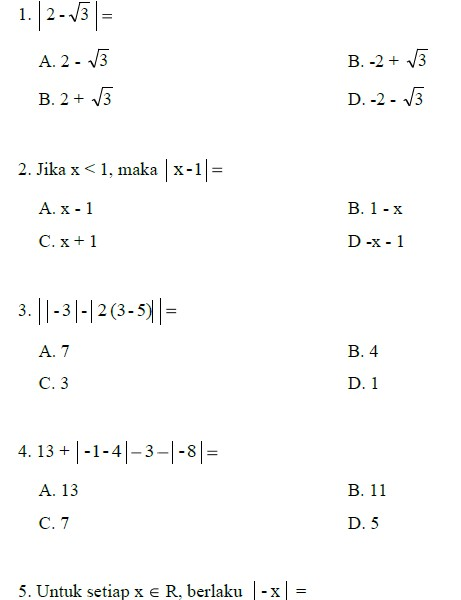
\includegraphics[width=3.22in, height=5.19in, keepaspectratio=false]{t17} 

\noindent \textbf{TES FORMATIF 1}
\textbf{ }

\noindent
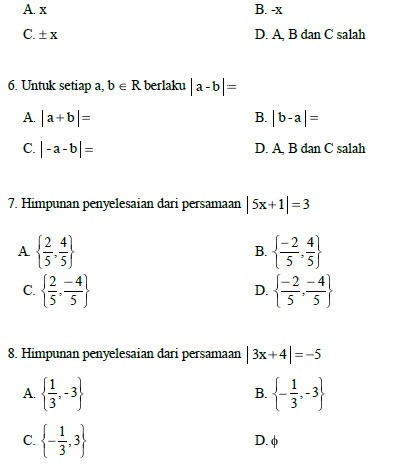
\includegraphics[width=3.28in, height=4.83in, keepaspectratio=false]{t18}
\noindent
\includegraphics*[width=3.37in, height=2.17in, keepaspectratio=false]{t19}

%------------------------------------------------

\section{Pertidaksamaan Nilai Mutlak Linear Satu Variabel}\index{Pertidaksamaan Nilai Mutlak Linear Satu Variabel}

\begin{enumerate}
\item  \textbf{KOMPETENSI INTI ( KI )}

\item \textbf{ }Memahami dan menerapkan pengetahuan faktual, konseptual, prosedural dalam ilmu pengetahuan, teknologi, seni, budaya, dan humaniora dengan wawasan kemanusiaan, kebangsaan, kenegaraan, dan peradaban terkait fenomena dan kejadian, serta menerapkan pengetahuan prosedural pada bidang kajian yang spesifik sesuai dengan bakat dan minatnya untuk memecahkan masalah

\item  Mencoba, mengolah, dan menyaji dalam ranah konkret dan ranah abstrak  terkait dengan pengembangan dari yang dipelajarinya di sekolah secara mandiri, dan mampu menggunakan metoda sesuai kaidah keilmuan
\end{enumerate}

\noindent 

\begin{enumerate}
\item  \textbf{KOMPETENSI DASAR ( KD )}
\end{enumerate}

\noindent 1.1  Mengintepretasi persamaan dan pertidaksamaan nilai mutlak dari bentuk linear satu variabel dengan persamaan dan pertidaksamaan linear Aljabar lainnya.

\noindent 1.2 Menyelesaikan masalah yang berkaitan dengan persamaan dan pertidaksamaan nilai mutlak dari bentuk linear satu variable

\noindent 

\begin{enumerate}
\item  \textbf{INDIKATOR PENCAPAIAN KOMPETENSI}

\item \textbf{ }Memahami dan menjelaskan konsep nilai mutlak.

\item  Menentukan penyelesaian persamaan nilai mutlak linear satu variabel.

\item  Menentukan penyelesaian pertidaksamaan nilai mutlak linear satu variabel.

\item  Menggunakan konsep nilai mutlak untuk menyelesaikan masalah kontekstual yang berkaitan dengan nilai mutlak.

\item  Menggunakan konsep persamaan dan pertidaksamaan untuk menentukan penyelesaian permasalahan nilai mutlak.
\end{enumerate}

\noindent \textbf{}

\begin{enumerate}
\item \textbf{ TUJUAN PEMBELAJARAN }

\item \textbf{ }Setelah membaca, berdiskusi dan menggali informasi, peserta didik akan dapat memahami dan menjelaskan konsep nilai mutlak dengan baik dan percaya diri.

\item  Setelah berdiskusi dan menggali informasi, peserta didik akan dapat menentukan penyelesaian persamaan nilai mutlak satu variable dengan percaya diri.

\item  Setelah berdiskusi dan menggali informasi, peserta didik akan dapat pertidaksamaan nilai mutlak satu variable dengan percaya diri.

\item  Disediakan permasalahan kontekstual dan LKS, peserta didik dapat menyelesaikan permasalahan tersebut dengan konsep nilai mutlak secara mandiri.

\item  Disediakan permasalahan nilai mutlak dan LKS, peserta didik dapat menyelesaikan persmasalahan nilai mutlak dengan menggunakan konsep persamaan dan pertidaksaman secara mandiri.
\end{enumerate}

\noindent 

\noindent \textbf{MATERI PEMBELAJARAN}

\noindent Pertidaksamaan~adalah kalimat/pernyataan matematika yang menunjukkan perbandingan ukuran dua objek atau lebih dan dihubungkan oleh satu dari beberapa simbol berikut :

\begin{enumerate}
\item  $<$ (kurang dari)

\item  $>$ (lebih dari)

\item  $\mathrm{\le}$ (kurang dari atau sama dengan)

\item  $\mathrm{\ge}$ (lebih dari atau sama dengan)
\end{enumerate}

\noindent Nilai Mutlak~adalah nilai suatu bilangan yang dihitung dari jarak bilangan itu dengan nol (0), sehingga bilangan yang dinilaimutlakkan selalu bernilai positif.\textbf{}

\begin{enumerate}
\item \begin{enumerate}
\item \textbf{ Konsep Nilai Mutlak}
\end{enumerate}
\end{enumerate}

\noindent Untuk memahami konsep nilai mutlak, akan diilustrasikan dengan cerita berikut ini: Seorang anak pramuka sedang latihan baris berbaris. Dari posisi diam, si anak diminta maju 2 langkah ke depan, kemudian 4 langkah ke belakang. Dilanjutkan dengan 3 langkah ke depan dan akhirnya 2 langkah ke belakang. Dari cerita di atas dapat diambil permasalahan :

\begin{enumerate}
\item \begin{enumerate}
\item \begin{enumerate}
\item  Berapakah banyaknya langkah anak pramuka tersebut dari pertama sampai terakhir ?

\item  Dimanakah posisi terakhir anak pramuka tersebut, jika diukur dari posisi diam? (berapa langkah ke depan atau berapa langkah ke belakang) 
\end{enumerate}
\end{enumerate}
\end{enumerate}

\noindent  

\noindent Untuk menjawab permasalahan diatas, akan diberikan gambar garis bilangan berikut:

\noindent \includegraphics*[width=6.10in, height=2.28in, keepaspectratio=false]{td20}

\noindent Dari gambar di atas, kita misalkan bahwa x = 0 adalah posisi diam (awal) si anak. Anak panah ke kanan menunjukkan arah langkah ke depan (bernilai positif) dan anak panah ke kiri menunjukkan arah langkah ke belakang (bernilai negatif). Sehingga permasalahan di atas dapat dijawab sebagai berikut : 

\begin{enumerate}
\item  Banyaknya langkah anak pramuka  tersebut dari pertama sampai terakhir  adalah bentuk penjumlahan  2 + 4 + 3 + 2 = 11 langkah. Bentuk penjumlahan ini merupakan penjumlahan tampa memperhatikan arah ke depan (positif) dan ke belakang (negatif) 

\item  Dari gambar diatas, dapat dilihat bahwa posisi terakhir anak pramuka tersebut, jika diukur dari posisi diam adalah 1 langkah ke belakang (x = --1). Hasil ini didapat dari bentuk penjumlahan  2 + (--4) + 3 + (--1)  =  --1. Bentuk penjumlahan ini merupakan penjumlahan dengan memperhatikan arah ke depan (positif) dan ke belakang (negatif).  
\end{enumerate}

\noindent 

\noindent Ilustrasi dari penyelesaian soal (a) di atas merupakan dasar dari konsep nilai mutlak.Dimana \textbf{\textit{Nilai mutlak suatu bilangan real x merupakan jarak antara bilangan itu dengan nol pada garis bilangan}}. Dan dilambangkan dengan x. Secara formal nilai mutlak didefinisikan :

\noindent Misalkan x bilangan real, maka : $\left|x\right|=\left\{ \begin{array}{c}
\ \ \ x,\ \ \ \ \ \ \ jika\ x\ge 0 \\ 
\ -x,\ \ \ \ \ \ \ jika\ x<0 \end{array}
\right.$

\noindent 

\begin{enumerate}
\item \begin{enumerate}
\item  \textbf{Pertidaksamaan Nilai Mutlak Satu Variabel}
\end{enumerate}
\end{enumerate}

\noindent Pertidaksamaan dapat diselesaikan dengan menggunakan sifat-sifat berikut :

\noindent \textbf{Bentuk 1}

\begin{enumerate}
\item \textbf{ }$Jika\ \left|f\left(x\right)\right|<a,\ maka\ -a<f\left(x\right)<a\ $

\item  $Jika\ \left|f\left(x\right)\right|>a,\ maka\ \ f\left(x\right)<-a\ atau\ f\left(x\right)>a$
\end{enumerate}

\noindent \textbf{Bentuk 2}

\begin{enumerate}
\item \textbf{ }$Jika\ \left|f\left(x\right)\right|<g\left(x\right),\ maka\ f^2\left(x\right)<g^2\left(x\right),\ dengan\ syarat\ g\left(x\right)>0\ $

\item  $Jika\ \left|f\left(x\right)\right|>g\left(x\right),\ maka\ f^2\left(x\right)>g^2\left(x\right),\ dengan\ syarat\ g\left(x\right)>0\ $
\end{enumerate}

\noindent \textbf{Bentuk 3}

\begin{enumerate}
\item \textbf{ }$Jika\ \left|f\left(x\right)\right|<\left|g\left(x\right)\right|,\ maka\ f^2\left(x\right)<g^2\left(x\right)\ $

\item  $Jika\ \left|f\left(x\right)\right|>\left|g\left(x\right)\right|,\ maka\ f^2\left(x\right)>g^2\left(x\right)$
\end{enumerate}

\noindent 

\noindent Contoh :

\begin{enumerate}
\item  Tentukan interval nilai x yang memenuhi pertidaksamaan $\left|2x+3\right|<5$
\end{enumerate}

\noindent Jawab :
\[\left|2x+3\right|<5\] 
\[-5<2x+3<5\] 
\[-5-3<2x+3-3<5-3\] 
\[-8<2x<2\] 
\[-4<x<1\] 


\begin{enumerate}
\item  Tentukan interval nilai x yang memenuhi pertidaksamaan $\left|2x-9\right|<4x-3$
\end{enumerate}

\noindent Jawab :
\[\left|2x-9\right|<4x-3\] 
\[{\left(2x-9\right)}^2<{\left(4x-3\right)}^2\] 
\[4x^2-36x+81<16x^2-24x+9\] 
\[-12x^2-12x+72<0\] 
\[x^2+x-6>0\] 
\[\left(x+3\right)\left(x-2\right)>0\] 
$x<-3$ atau $x>2$ {\dots}{\dots}{\dots}{\dots}{\dots}{\dots}{\dots}{\dots}.. \eqref{GrindEQ__1_}

\noindent Syarat : $4x-3>0\ \ \Longrightarrow \ \ x>\frac{3}{4}$  {\dots}{\dots}{\dots} \eqref{GrindEQ__2_}

\noindent Dari \eqref{GrindEQ__1_} dan \eqref{GrindEQ__2_} diperoleh interval : $x>2$

\begin{enumerate}
\item  Tentukan interval nilai x yang memenuhi pertidaksamaan $\left|x+4\right|\ge \left|3x-8\right|$
\end{enumerate}

\noindent Jawab :
\[\left|x+4\right|\ge \left|3x-8\right|\] 
\[{\left(x+4\right)}^2\ge {\left(3x-8\right)}^2\] 
\[x^2+8x+16\ge {9x}^2-48x+64\] 
\[{-8x}^2+56x-48\ge 0\] 
\[x^2-7x+6\le 0\] 
\[1\le x\le 6\] 


\noindent 

\begin{enumerate}
\item \begin{enumerate}
\item  \textbf{Menemukan konsep nilai mutlak}
\end{enumerate}
\end{enumerate}

\noindent Nilai mutlak dari suatu bilangan adalah positif. Hal ini sama dengan akar dari sebuah bilangn selalu positif. Misal $a\in R$, maka $\sqrt{a^{2\ }}=\ \left|a\right|=\left\{ \begin{array}{c}
a,\ \ a\ge 0 \\ 
-a,\ \ a<0 \end{array}
\right.$ . Dengan demikian grafik fungsi nilai mutlak selalu berada di atas sumbu X.

\textbf{Konsep}

\noindent Persamaan dan pertidaksamaan linier dapat diperoleh dari persamaan atau fungsi nilai mutlak yang diberikan. 

\noindent Misalnya jika diketahui $\left|ax+b\right|=c,\ untuk\ a,\ b,\ c\ \in R$, 

\noindent maka menurut definisi nilai mutlak  diperoleh persamaan $ax+b=c.$ 

\noindent Demikian juga untuk pertidaksamaan linier.

\noindent \textbf{Prinsip}

\begin{enumerate}
\item \textbf{ }Bentuk umum dari persamaan linier dinyatakan : $a_1x_1+\ a_2x_2+a_3x_3+\dots .+a_nx_n=0$ dengan setiap koefesien dan variable-variabelnya merupakan bilangan-bilangan rill. Jika a${}_{2}$ = a${}_{3}$ = {\dots}..= a${}_{n}$ = 0, maka diperoleh persamaan linier satu variable dan apabila a${}_{3}$ = a${}_{4}$ = {\dots}.= a${}_{n}$ = 0 maka diperoleh persamaan linier dua variable. 

\item  Pertidaksamaan linier adalah suatu  kalimat terbuka yang menggunakan tanda pertidaksamaan $<$, $\mathrm{\le}$, $>$, dan  $\mathrm{\ge}$. $a_1x_1+\ a_2x_2+a_3x_3+\dots .+a_nx_n>0$ dengan setiap koefesien dan variable- variabelnya merupakan bilangan-bilangan rill. Jika a${}_{2}$ = a${}_{3}$ = {\dots}..= a${}_{n}$ = 0, maka diperoleh pertidaksamaan linier satu variable dan apabila a${}_{3}$ = a${}_{4}$ = {\dots}.= a${}_{n}$ = 0 maka diperoleh pertidaksamaan linier dua variableBentuk umum dari persamaan linier dinyatakan : 
\end{enumerate}

\noindent $a_1x_1+\ a_2x_2+a_3x_3+\dots .+a_nx_n=0$ dengan setiap koefesien dan variable-variabelnya merupakan bilangan-bilangan rill. Jika a${}_{2}$ = a${}_{3}$ = {\dots}..= a${}_{n}$ = 0, maka diperoleh persamaan linier satu variable dan apabila a${}_{3}$ = a${}_{4}$ = {\dots}.= a${}_{n}$ = 0 maka diperoleh persamaan linier dua variable.

\begin{enumerate}
\item  Himpunan penyelesaian suatu persamaan dan pertidaksamaan linier adalah suatu himpunan yang anggotanya nilai variable yang memenuhi persamaan atau pertidaksamaan tersebut. Banyak anggota himpunan penyelesaiannya sebuah persamaan dapat :
\end{enumerate}

\noindent  \eqref{GrindEQ__1_} tepat satu,

\noindent  \eqref{GrindEQ__2_} lebih dari satu (berhingga atau tak berhingga banyak penyelesaian, atau

\noindent  \eqref{GrindEQ__3_} tidak punya penyelesaian.

\noindent \textbf{4. Pertidaksamaan Linier Satu Variabel}

\noindent Pertidaksamaan adalah kalimat terbuka yang menggunakan lambing $<$, $>$, $\mathrm{\ge}$, dan~ $\mathrm{\le}$ . ~Contohnya bentuk pertidaksamaan : y + 7 $<$ 7 dan 2y + 1 $>$ y + 4. Pertidaksamaan linier dengan satu variable adalah suatu kalimat terbuka yang hanya memuat satu variable dengan derajad satu, yang dihubungkan oleh lambang $<$, $>$, $\mathrm{\ge}$, dan~ $\mathrm{\le}$. Variablenya hanya satu yaitu y dan berderajad satu. Pertidaksamaan yang demikian disebut pertidaksamaan linier dengan satu variable (peubah).

\noindent \textbf{Menentukan Himpunan Penyelesaian Pertidaksamaan Linier Satu variable}

\noindent Sifat- sifat pertidaksamaan adalah :

\noindent 1.~~~~~~Jika pada suatu pertidaksamaan kedua ruasnya ditambah atau dikurang dengan bilangan yang sama, maka akan diperoleh pertidaksamaan baru yang ekuivalen dengan pertidaksamaan semula

\noindent 2.~~~~~~Jika pada suatu pertidaksamaan dikalikan dengan bilangan positif , maka akan diperoleh pertidaksamaan baru yang ekuivalen dengan pertidaksamaan semula

\noindent 3.~~~~~~Jika pada suatu pertidaksamaan dikalikan dengan bilangan negatif , maka akan diperoleh pertidaksamaan baru yang ekuivalen dengan pertidaksamaan semula bila arah dari tanda ketidaksamaan dibalik ~

\noindent 4.~~~~~~Jika pertidaksamaannya mengandung pecahan, cara menyelesaikannya adalah mengalikan kedua ruasnya dengan KPK penyebut-penyebutnya sehingga penyebutnya hilang .

\noindent \textbf{}

\noindent \textbf{Menyelesaikan Pertidaksamaan Nilai Mutlak}Menyelesaikan pertidaksamaan nilai mutlak caranya hampir sama dengan persamaan nilai mutlak. hanya saja berbeda sedikit pada tanda ketidaksamaannya. Langkah-langkah selanjutnya seperti menyelesaikan pertidaksamaan linear atau kuadrat satu variabel .Pertidaksamaan~ mutlak dapat digambarkan sebagai berikut.

\noindent \includegraphics*[width=4.15in, height=0.77in, keepaspectratio=false]{td21}

\noindent Apabila fungsi di dalam nilai mutlak berbentuk ax + b maka pertidaksamaan nilai mutlak dapat diselesaikan seperti berikut.

\noindent \includegraphics*[width=4.76in, height=0.77in, keepaspectratio=false]{td22}Lebih jelasnya perhatikan contoh berikut ini.

\noindent \textbf{Contoh 1 :}

\noindent ~Tentukan himpunan penyelesaian 3x -- 7 $>$ 2x + 2 jika x merupakan anggota $\{$1,2,3,4,{\dots} ,15$\}$

\noindent 

\noindent 

\noindent 

\noindent Jawab :

\noindent 3x -- 7 $>$ 2x + 2; x ? $\{$1, 2, 3, 4{\dots} 15$\}$

\noindent 3x --2x -- 7 $>$ 2x - 2x + 2 ~~~~~~~~~~~~~~~~~~~~~~~~~~~~~~~~~~~~~~~~~~~ ( kedua ruas dikurangi 2x)

\noindent x -- 7 $>$ 2

\noindent x -- 7 + 7 $>$ 2 + 7~~~~~~~~~~~~~~~~~~~~~~~~~~~~~~~~~~~~~~~~~~~~~~~~~~~~~~~~ ( kedua ruas dikurangi7 )~~~~~~~

\noindent x $>$ 9

\noindent 

\noindent jadi himpunan penyelesaiannya adalah $\{$x {\textbar} x $>$ 9 ; x bilangan asli $\mathrm{\le}$ 15$\}$

\noindent HP = $\{$10, 11, 12, 13, 14, 15$\}$

\noindent \textbf{}

\noindent \textbf{Contoh 2 :}

\noindent Tentukan himpunan penyelesaian dari pertidaksamaan 3x -- 1 $<$ x + 3~ dengan x variable pada himpunan bilangan cacah.

\noindent Jawab :

\noindent 3x -- 1 $<$ x + 3

\noindent 3x -- 1+ 1 $<$ x + 3 + 1 ~~~~~~~~~~~~ (kedua ruas ditambah 1 )

\noindent 3x $<$ x + 4~

\noindent 3x + (-x) $<$ x + (-x) +4~ ~~~~~~~~~~~~~~~~~~~~~~ (kedua ruas ditambah -- x)

\noindent 2x $<$ 4

\noindent X $<$ 2

\noindent Karena x anggota bilangan cacah maka yang memenuhi x $<$ 2 adalah x = 0 atau x = 1

\noindent Jadi himpunan pnyelesaiannya adalah $\{$ 0,1 $\}$ .

\noindent \textbf{}

\noindent \textbf{Contoh 3 :}

\noindent Sebuah perahu angkut dapat menampung dengan berat tidak lebih dari 1~~ton . jika sebuah kotak beratnya 15 kg, maka berapa paling banyak kotak yang dapat diangkut oleh perahu ?

\noindent Jawab :

\noindent Kalimat matematika : 15 kg x $\mathrm{\le}$ 1~~ton

\noindent Penyelesaian : 15 kg x $\mathrm{\le}$ 1 .500 kg

\noindent ~~~~~~~~~~~~~~~~~~~~~~~ ~~~~~~~ x $\mathrm{\le}$ 1 .500 kg

\noindent ~~~~~~~~~~~~~~~~~~~~~~~~~~~~~~~~~~~~~~~~~~~~~ 15 kg

\noindent ~~~~~~~~~~~~~~~~~~~~~~~~~~~~~~~~~~~~ x $\mathrm{\le}$~~~~ 100

\noindent jadi perahu paling banyak mengangkut 100 kotak~ .~~~~~~

\noindent \textbf{Contoh 4 :}

\noindent Jarak terpendek yang diperlukan untuk menghentikan suatu mobil sejak pengereman dilakukan disebut jarak henti. Jarak henti ini merupakan faktor penting yang perlu diuji sebelum peluncuran produk mobil baru. Data mengenai jarak henti dapat digunakan untuk menghitung waktu reaksi pengemudi (selang waktu mulai pengemudi melihat kejadian sampai dia bereaksi menginjak pada rem) berdasarkan tingkat kelajuan mobil (dalam meter/jam).

\noindent Suatu penelitian menyatakan bahwa jarak henti dapat dinyatakan dengan formula :d = {\textbar}0,44v2~+ 1,1v{\textbar}, dimana v adalah kelajuan dan d dalam meter.

\noindent Pada batas kelajuan berapakah jarak henti mobil lebih dari 100 meter?

\noindent \textit{Penyelesaian :}

\noindent Oleh karena kelajuan selalu bernilai positif, maka~{\textbar}0,44v2~+ 1,1v{\textbar} = 0,44v2~+ 1,1v. Selanjutnya, agar jarak henti mobil lebih dari 100 meter, maka d haruslah lebih besar dari seratus.

\noindent \includegraphics*[width=3.04in, height=3.99in, keepaspectratio=false]{td23.PNG}\textbf{}

\noindent Jadi, batas kelajuannya jarak henti mobil lebih dari 100 meter adalah~\textbf{-16,4 $\boldsymbol{<}$ v $\boldsymbol{<}$ 13,9 meter/jam}.

\noindent \textbf{Contoh 5 :}

\noindent Selisih antara panjang dan lebar suatu persegi panjang kurang dari 6 cm. Jika keliling persegi panjang adalah 32 cm, maka tentukan batas nilai lebar persegi panjang tersebut!

\noindent \textit{Penyelesaian :}

\noindent Oleh karena keliling persegi panjang adalah 32 cm, maka \textit{2(p + l) = 32} $<$=$>$~\textit{p + l }

\noindent \textit{= 16} $<$=$>$~\textit{p = 16-l}

\noindent Selanjutnya, karena selisih antara panjang dan lebar persegi kurang dari 6 cm, maka

\noindent \includegraphics*[width=2.13in, height=1.97in, keepaspectratio=false]{td24.PNG}

\noindent Dengan demikian, batas nilai lebar persegi panjang yang dimaksud adalah antara 5 cm sampai dengan 11 cm.

\noindent \textbf{Contoh 6 :}

\noindent Pergerakan suatu titik dalam koordinat kartesius ditentukan oleh nilai absis dan memenuhi pertidaksamaan~{\textbar}x -- 1{\textbar}2~+ 2{\textbar}x -- 1{\textbar} $<$ 15. Tentukan nilai x yang memenuhi pertidaksamaan tersebut!

\noindent \textit{Penyelesaian :}

\noindent Jika dimiisalkan~{\textbar}x -- 1{\textbar} = p, maka diperoleh hasil sebagai berikut :

\noindent \includegraphics*[width=3.79in, height=3.40in, keepaspectratio=false]{td25.PNG}\textbf{}

\noindent jadi, nilai x yang memenuhi adalah~\textbf{$\boldsymbol{\{}$ x $\boldsymbol{\mathrm{\in }}$ $\boldsymbol{\mathrm{\mathbb{R}}}$ {\textbar} -2 $\boldsymbol{<}$ x $\boldsymbol{<}$ 4 $\boldsymbol{\}}$}.

\noindent \textbf{}

\noindent \textbf{Mengubah soal cerita ke bentuk pertidaksamaan linear}

\noindent Pertidaksamaan Linear adalah peridaksamaan yang memiliki variabel atau peubah yang berderajat satu. Pada kesempatan sebelumnya telah dibahas bagaimana penyelesaian pertidaksamaan linear satu variabel. Berdasarkan prinsip penyelesaian tersebut, pertidaksamaan linear ternyata dapat diaplikasikan dalam kehidupan sehari-hari, yaitu untuk menyelesaikan berbagai persoalan atau perhitungan yang melibatkan pertidaksamaan. Beberapa perhitungan matematika dapat diterjemahkan ke dalam model matematika berbentuk pertidaksamaan satu variabel. Soal tersebut dapat diubah ke pertidaksamaannilai mutlak sesuai model soalnya. Pada kesempatan ini, bahan belajar sekolah akan membahas bagaimana cara mengubah soal cerita ke bentuk pertidaksamaan linear dan menentukan penyelesaiannya.

\noindent \textbf{Bentuk Pertidaksamaan Linear}

Setiap masalah memiliki bentuknya masing-masing. Tidak sesuai soal dapat diselesaikan dengan model matematika berbentuk pertidaksamaan linear. Oleh karena itu, untuk menyelesaikan suatu permasalahan kita harus mengidentifikasi bentuk pertidaksamaan yang paling relevan dengan masalah tersebut.

 Karena kita berbicara tentang pertidaksamaan linear, maka kita harus terlebih dahulu memahami ciri dari pertidaksamaan linear dan mengenali ciri-ciri soal yang berkaitan dengan pertidaksamaan linear. Salah satu ciri utama yang dapat kita lihat adalah penggunaan kata-kata pertidaksamaan. Dalam Soal cerita, hubungan pertidaksamaan seringkali dihadirkan dengan penggunaan kata-kata seperti kurang dari, sebanyak-banyaknya, maksimal, dan sebagainya. Kata-kata tersebut merupakan indikasi bahwa soal tersebut berbentuk pertidaksamaan. Selanjutnya, kita harus mengidentifikasi kondisi yang diketahui dalam soal. Kita harus mengidentifikasi besaran yang digunakan dalam soal dan selanjutnya menyatakan besaran tersebut sebagai variabel. Setelah itu, kita susunlah pertidaksamaan yang sesuai dengan soal. Sebagai acuan, kita harus memahami bentuk umum atau bentuk baku dari pertidaksamaan yang ingin kita gunakan. Karena kita membahas pertidaksamaan linear satu variabel, maka kita harus memahami bentuk baku dari pertidaksamaan linear satu variabel. 

\noindent Bentuk baku pertidaksamaan linear satu variabel dalam variabel x :

\begin{enumerate}
\item  Pertidaksamaan kurang dari : ax + b $<$ 0 

\item  Pertidaksamaan kurang dari sama dengan : ax + b $\mathrm{\le}$ 0

\item  Pertidaksamaan lebih dari : ax + b $>$ 0 

\item  Pertidaksamaan lebih dari sama dengan : ax + b $\ge $ 0
\end{enumerate}

\noindent Pada bentuk di atas, x merupakan variabel atau peubah sedangkan a dan b merupakan bilangan-bilangan real. Nilai a dan b diperoleh dari soal cerita sehingga bentuk pertidaksamaannya akan bergantung pada soal ceritanya.

\noindent Suatu pertidaksamaan linear satu variabel dapat diselesaikan dengan metode manipulasi aljabar. Dalam memanipulasi aljabar pertidaksamaan linear, ada aturan atau sifat-sifat yang harus diperhatikan. 

\noindent \textbf{Menyelesaikan soal cerita berbentuk pertidaksamaan linear}

\noindent Untuk menyelesaikan suatu soal cerita, kita harus memastikan bentuk pertidaksamaan yang sesuai. Jika soal cerita sudah dipastikan berbentuk pertidaksamaan linear satu variabel, maka soal tersebut dapat kita selesaikan dengan prinsip penyelesaian pertidaksamaan linear.

\noindent Langkah pertama yang harus kita lakukan adalah mengidentifikasi besaran yang tidak diketahui nilainya dalam soal. Besaran inilah yang nanti akan kita nyatakan sebagai variabel. Kemudian kita identifikasi nilai-nilai yang diketahui dalam soal dan hubungan pertidaksamaan yang digunakan.

\noindent Selanjutnya kita lakukan pemisalan untuk menyatakan besaran sebagai variabel. Kita bisa menggunakan symbol huruf abjad yang paling relevan dengan besaran tersebut kemudian kita susun bentuk pertidaksamaannya berdasarkan nilai-nilai yang diketahui dalam soal.

\noindent Setelah dihasilkan bentuk pertidaksamaan linear satu variabel, selanjutnya kita selesaikan pertidaksamaan tersebut dengan prinsip manipulasi aljabar. Dalam manipulasi ini kita harus memperhatikan sifat-sifat perubahan tanda pertidaksamaan.

\noindent Berdasarkan uraian diatas, maka berikut langkah menyelesaikan soal cerita yang berbentuk pertidaksamaan linear satu variabel:

\begin{enumerate}
\item  Identifikasi besaran yang tidak diketahui dalam soal

\item  Nyatakan besaran tersebut sebagai variabel

\item  Identifikasi hubungan pertidaksamaan yang digunakan

\item  Susun pertidaksamaan linear satu variabel sesuai soal 

\item  Tentukan penyelesaian pertidaksamaannya.
\end{enumerate}

\noindent \textbf{Contoh Soal Cerita}

\noindent Jumlah dua bilangan tidak kurang dari 400. Jika bilangan pertama sama dengan empat kali bilangan kedua, maka tentukanlah batas-batas nilai dari kedua bilangan tersebut.

\noindent \textbf{Pembahasan :}

\noindent Langkah pertama, kita identifikasi besaran yang belum diketahui. Besaran tersebut adalah bilangan pertama dan bilangan kedua. Selanjutnya kita misalkan bilangan pertama dan bilangan kedua sebagai variabel.

\noindent Misalkan :

\noindent Bilangan pertama = x

\noindent Bilangan kedua = y 

\noindent Dari soal diketahui kalau bilangan pertama sama dengan empat kali bilangan kedua, dengan demikian berlaku hubungan x=4y 

\noindent 

\noindent Selanjutnya diketahui bahwa jumlah kedua bilangan tersebut tidak kurang dari 400. Kata ``Tidak kurang'' dalam soal merupakan indikasi hubungan pertidaksamaan lebih besar sama dengan ($\mathrm{\ge}$). Itu artinya, model pertidaksamaannya adalah pertidaksamaan lebih dari sama dengan.

\noindent 

\noindent Berdasarkan kondisi yang diketahui dalam soal, maka bentuk pertidaksamaan yang sesuai dengan soal adalah sebagai berikut :

\begin{enumerate}
\item  x + y $\mathrm{\ge}$ 400
\end{enumerate}

\noindent Karena x = 4y, maka pertidaksamaannya menjadi:

\begin{enumerate}
\item  4y + y $\mathrm{\ge}$ 400

\item  5y $\mathrm{\ge}$ 400
\end{enumerate}

\noindent 

\noindent Selanjutnya, kita selesaikan pertidaksamaan linear tersebut dengan manipulasi aljabar yaitu dengan membagi kedua ruas dengan 5 sehingga diperoleh :

\begin{enumerate}
\item  5y $\mathrm{\ge}$ 400

\item  y $\mathrm{\ge}$ 80
\end{enumerate}

\noindent Karena kedua ruas sama-sama dibagi 5 (bilangan positif), maka tanda pertidaksamaannya tetap. Nilai y di atas merupakan batas nilai untuk bilangan kedua.

\noindent Selanjutnya kita tentukan batas nilai untuk bilangan pertama:

\begin{enumerate}
\item  x + y $\mathrm{\ge}$ 400

\item  x + 80 $\mathrm{\ge}$ 400

\item  x + 80 -- 80 $\mathrm{\ge}$ 400 -- 80 

\item  x $\mathrm{\ge}$ 320
\end{enumerate}

\noindent Jadi, batas nilai untuk bilangan pertama tidak kurang dari 80 dan batas nilai untuk bilangan kedua tidak kurang dari 320.

%------------------------------------------------

%----------------------------------------------------------------------------------------
%	CHAPTER 2
%----------------------------------------------------------------------------------------

\chapter{Linear Tiga Variabel}

\section{SISTEM PERSAMAAN LINEAR TIGA VARIABEL}\index{SISTEM PERSAMAAN LINEAR TIGA VARIABEL}

\noindent \textbf{SISTEM PERSAMAAN LINEAR TIGA VARIABEL (SPLTV)}

\noindent Sistem persamaan linear tiga variabel adalah sistem persamaan yang terdiri dari tiga persamaan dimana masing-masing persamaan memiliki tiga variabel. Contoh SPLTV dengan variabel~\includegraphics*[width=0.25in, height=0.10in, keepaspectratio=false]{image52}~dan~\includegraphics*[width=0.08in, height=0.07in, keepaspectratio=false]{image53}:

\noindent \includegraphics*[width=1.82in, height=0.73in, keepaspectratio=false]{image15}

\noindent dimana~\includegraphics*[width=0.39in, height=0.15in, keepaspectratio=false]{image16}~dan~\includegraphics*[width=0.09in, height=0.11in, keepaspectratio=false]{image17}~adalah bilangan-bilangan real.

\noindent Pada SPLTV terdapat 2 cara penyelesaian, yaitu:

\begin{enumerate}
\item  Metode Subtitusi
\end{enumerate}

\noindent Langkah yang dilakukan pada metode ini yaitu:

\begin{enumerate}
\item  Ubah salah satu persamaan yang ada pada sistem dan nyatakan~\includegraphics*[width=0.09in, height=0.07in, keepaspectratio=false]{image18}~sebagai fungsi dari~\includegraphics*[width=0.08in, height=0.10in, keepaspectratio=false]{image19}~dan~\includegraphics*[width=0.08in, height=0.07in, keepaspectratio=false]{image20}, atau~\includegraphics*[width=0.08in, height=0.10in, keepaspectratio=false]{image21}~sebagai fungsi dari~\includegraphics*[width=0.09in, height=0.07in, keepaspectratio=false]{image22}~dan~\includegraphics*[width=0.08in, height=0.07in, keepaspectratio=false]{image23}, atau~\includegraphics*[width=0.08in, height=0.07in, keepaspectratio=false]{image24}~sebagai fungsi dari~\includegraphics*[width=0.09in, height=0.07in, keepaspectratio=false]{image25}~dan~\includegraphics*[width=0.08in, height=0.10in, keepaspectratio=false]{image26}..

\item  Subtitusikan fungsi~\includegraphics*[width=0.09in, height=0.07in, keepaspectratio=false]{image27}~atau~\includegraphics*[width=0.08in, height=0.10in, keepaspectratio=false]{image28}~atau~\includegraphics*[width=0.08in, height=0.07in, keepaspectratio=false]{image29}~dari langkah pertama pada dua persamaan yang lain, sehingga diperoleh SPLDV.

\item  Selesaikan SPLDV yang diperoleh dengan metode yang dibahas pada penyelesaian SPLDV di atas.
\end{enumerate}

\noindent Contoh Soal:Tentukan penyelesaian dari sistem persamaan linear tiga variabel berikut:

\noindent \includegraphics*[width=2.03in, height=0.73in, keepaspectratio=false]{image30}.

\noindent Jawab:

\noindent Langkah pertama, nyatakan persamaan (I) menjadi fungsi dari~\includegraphics*[width=0.09in, height=0.07in, keepaspectratio=false]{image31}, yaitu:~\includegraphics*[width=2.44in, height=0.16in, keepaspectratio=false]{image32}. Kemudian subtitusikan pada persamaan (II) dan (III), menjadi

\noindent Persamaan (II):~\includegraphics*[width=1.97in, height=0.19in, keepaspectratio=false]{image33}

\noindent Selesaikan, didapat:~\includegraphics*[width=1.69in, height=0.19in, keepaspectratio=false]{image34}

\noindent Persamaan (III):~\includegraphics*[width=2.06in, height=0.19in, keepaspectratio=false]{image35}

\noindent Selesaikan, didapat:~\includegraphics*[width=1.08in, height=0.16in, keepaspectratio=false]{image36}~atau~\includegraphics*[width=1.34in, height=0.19in, keepaspectratio=false]{image37}.

\noindent Persamaan (IV) dan (V) membentuk SPLDV

\noindent Dari persamaan (V),~\includegraphics*[width=1.80in, height=0.16in, keepaspectratio=false]{image38}, kemudian disubtitusikan pada persamaan (IV), menjadi:

\noindent \includegraphics*[width=1.51in, height=0.19in, keepaspectratio=false]{image39}

\noindent \includegraphics*[width=1.47in, height=0.15in, keepaspectratio=false]{image40}

\noindent \includegraphics*[width=0.56in, height=0.55in, keepaspectratio=false]{image41}

\noindent Kemudian subtitusikan~\includegraphics*[width=0.40in, height=0.17in, keepaspectratio=false]{image42}~pada persamaan~\includegraphics*[width=0.70in, height=0.16in, keepaspectratio=false]{image43}~diperoleh\includegraphics*[width=0.70in, height=0.17in, keepaspectratio=false]{image44}~atau~\includegraphics*[width=0.40in, height=0.16in, keepaspectratio=false]{image45}.

\noindent Subtitusikan~\includegraphics*[width=0.40in, height=0.14in, keepaspectratio=false]{image46}~dan~\includegraphics*[width=0.40in, height=0.12in, keepaspectratio=false]{image47}~pada persamaan~\includegraphics*[width=1.08in, height=0.16in, keepaspectratio=false]{image48}, menjadi~\includegraphics*[width=1.21in, height=0.19in, keepaspectratio=false]{image49}, diperoleh~\includegraphics*[width=0.41in, height=0.14in, keepaspectratio=false]{image50}.

\noindent Sehingga himpunan penyelesaian adalah~\includegraphics*[width=0.56in, height=0.18in, keepaspectratio=false]{image51}

\begin{enumerate}
\item  Metode Eliminasi
\end{enumerate}

\noindent Langkah penyelesaian pada metode eliminasi yaitu:

\begin{enumerate}
\item  Eliminasi salah satu variabel sehingga diperoleh SPLDV

\item  Selesaikan SPLDV yang diperoleh dengan langkah seperti pada penyelesaian SPLDV yang telah dibahas

\item  Subtitusikan variabel yang telah diperoleh pada persamaan yang ada.
\end{enumerate}

\noindent 

\noindent 

\noindent 

\noindent 

\noindent Metoda meyelesaikan persamaan

\noindent 1. Metoda Eliminasi

\noindent 2. Metoda subtitusi

\noindent 3. Metoda determinan

\noindent 4. Metoda matriks

\noindent 5. Metoda operasi baris elementer

\noindent ~

\noindent Metoda Eliminasi

\noindent Supaya lebih mudah langsung saja kita masuk ke contoh-contoh

\noindent Contoh soal 1 :

\noindent 2x + 3y -- z = 20

\noindent 3x + 2y + z = 20

\noindent x + 4y + 2z = 15

\noindent Jawab :

\noindent Ketiga persamaan bisa kita beri nama persamaan \eqref{GrindEQ__1_}, \eqref{GrindEQ__2_}, dan \eqref{GrindEQ__3_}

\noindent 2x + 3y -- z = 20 {\dots}{\dots}{\dots}{\dots}{\dots}{\dots}{\dots}{\dots}{\dots}..\eqref{GrindEQ__1_}

\noindent 3x + 2y + z = 20 {\dots}{\dots}{\dots}{\dots}{\dots}{\dots}{\dots}{\dots}{\dots}..\eqref{GrindEQ__2_}

\noindent x + 4y + 2z = 15 {\dots}{\dots}{\dots}{\dots}{\dots}{\dots}{\dots}{\dots}{\dots}..\eqref{GrindEQ__3_}

\noindent Sistem persamaan ini harus kita sederhanakan menjadi sistem persamaan linear 2 variabel. Untuk itu kita eliminasi variabel z

\noindent Sekarang persamaan \eqref{GrindEQ__1_} dan \eqref{GrindEQ__2_} kita jumlahkan

\noindent 2x + 3y -- z = 20

\noindent 3x + 2y + z = 20\_\_\_\_\_~~ +

\noindent 5x + 5y = 40

\noindent x + y = 8 {\dots}{\dots}{\dots}{\dots}{\dots}{\dots}{\dots}.\eqref{GrindEQ__4_}

\noindent Selanjutnya persamaan \eqref{GrindEQ__2_} dikali \eqref{GrindEQ__2_} dan persamaan \eqref{GrindEQ__3_} dikali \eqref{GrindEQ__1_} sehingga diperoleh

\noindent 6x + 4y + 2z = 40

\noindent x + 4y + 2z = 15\_\_\_\_~ \_

\noindent ~~~~~~~~~~~~~~ 5x = 25

\noindent ~~~~~~~~~~~~~~~~ x = 5

\noindent Nilai x ini kita subtitusi ke persamaan \eqref{GrindEQ__4_} sehingga

\noindent x + y = 8

\noindent 5 + y = 8

\noindent ~ ~ ~~ y = 3

\noindent selanjutnya nilai x dan y yang ada kita subtitusikan ke persamaan \eqref{GrindEQ__2_}

\noindent 3x + 2y + z = 20

\noindent 3.5 + 2.3 + z = 20

\noindent 15 + 6 + z = 20

\noindent ~~~~~~~~~~~~~~ z = -1

\noindent Jadi, himpunan penyelesaiannya adalah~$\{$(5, 3, -1)$\}$

\noindent Contoh soal 2 :

\noindent Tentukan himpunan penyelesaian dari

\noindent 3x + 4y -- 3z = 3

\noindent 2x -- y + 4z = 21

\noindent 5x + 2y + 6z = 46

\noindent Jawab :

\noindent Agar lebih mudah, ketiga persamaan kita beri nama \eqref{GrindEQ__1_}, \eqref{GrindEQ__2_}, dan \eqref{GrindEQ__3_}

\noindent 3x + 4y -- 3z = 3~ {\dots}{\dots}{\dots}{\dots}{\dots}{\dots}{\dots}{\dots}{\dots}{\dots}{\dots}.\eqref{GrindEQ__1_}

\noindent 2x -- y + 4z = 21~ {\dots}{\dots}{\dots}{\dots}{\dots}{\dots}{\dots}{\dots}{\dots}{\dots}{\dots}.\eqref{GrindEQ__2_}

\noindent 5x + 2y + 6z = 46 {\dots}{\dots}{\dots}{\dots}{\dots}{\dots}{\dots}{\dots}{\dots}{\dots}{\dots}.\eqref{GrindEQ__3_}

\noindent Selanjutnya persamaan \eqref{GrindEQ__1_} dikali 1 dan persamaan \eqref{GrindEQ__2_} dikali 4, sehingga diperoleh

\noindent 3x + 4y -- 3z = 3~~~ {\textbar}1{\textbar} $\mathrm{\to}$ 3x + 4y -- 3z = 3

\noindent 2x -- y + 4z = 21~~~ {\textbar}4{\textbar} $\mathrm{\to}$ 8x -- 4y+16z = 84 ~~ +

\noindent .~~~~~~~~~~~~~~~~~~~~~~~~~~~~~~~~~ 11x + 13z = 87 {\dots}{\dots}{\dots}{\dots}{\dots}..\eqref{GrindEQ__4_}

\noindent Berikutnya persamaan \eqref{GrindEQ__3_} dikali 1 dan persamaan \eqref{GrindEQ__2_} dikali 2, sehingga diperoleh

\noindent 5x + 2y + 6z = 46~~~ {\textbar}1{\textbar} $\mathrm{\to}$ 5x + 2y + 6z = 46

\noindent 2x -- y + 4z = 21~~~~~ {\textbar}2{\textbar} $\mathrm{\to}$ 4x -- 2y + 8z = 42~~~~ +

\noindent .~~~~~~~~~~~~~~~~~~~~~~~~~~~~~~~~~~~ 9x + 14z = 88 {\dots}{\dots}{\dots}{\dots}..\eqref{GrindEQ__5_}

\noindent Sekarang persamaan \eqref{GrindEQ__5_} dikali 11 dan persamaan \eqref{GrindEQ__4_} dikali 9 sehingga diperoleh

\noindent 9x + 14z = 88~~ {\textbar}11{\textbar}~~ 99x +154z = 968

\noindent 11x + 13z = 87~ {\textbar}9{\textbar}~~~ 99x + 117z=783~~~~~~ \_

\noindent .~~~~~~~~~~~~~~~~~~~~~~~~~~~~~~~~~~~~~ 37z = 185

\noindent .~~~~~~~~~~~~~~~~~~~~~~~~~~~~~~~~~~~~~~~~~ z = 5

\noindent Nilai z=5 kita subtitusi ke persamaan \eqref{GrindEQ__4_}

\noindent 11x + 13z = 87

\noindent 11x + 13.5 = 87

\noindent 11x + 65 = 87

\noindent ~~~~~~~~ 11x = 22

\noindent ~~~~~~~~~~~~~ x = 2

\noindent Nilai x=2 dan z=5 kita subtitusikan ke persamaan \eqref{GrindEQ__3_} sehingga

\noindent 5x +2y +6z = 46

\noindent 5.2 +2y +6.5 = 46

\noindent 10 + 2y + 30 = 46

\noindent ~~~~~~~~~~~~~~~~~ 2y = 6

\noindent ~~~~~~~~~~~~~~~~~~~ y = 3

\noindent Jadi, himpunan penyelesaiannya adalah~$\{$(2, 3, 5)$\}$

\noindent 

\noindent 1.\includegraphics*[width=3.12in, height=1.49in, keepaspectratio=false]{image61}Penyelesaian:\includegraphics*[width=3.13in, height=2.26in, keepaspectratio=false]{image62}\includegraphics*[width=3.11in, height=1.81in, keepaspectratio=false]{image63}

\noindent 2.\includegraphics*[width=2.89in, height=2.03in, keepaspectratio=false]{image64}Penyelesaian:\includegraphics*[width=3.11in, height=1.85in, keepaspectratio=false]{image65}\includegraphics*[width=3.12in, height=1.60in, keepaspectratio=false]{image66}\includegraphics*[width=3.12in, height=1.71in, keepaspectratio=false]{image67}

\noindent 

\noindent 

\noindent

%------------------------------------------------

\section{Penerapan Sistem Persamaan Linear Tiga Variabel}\index{Penerapan Sistem Persamaan Linear Tiga Variabel}


\noindent \textbf{CONTOH SOAL PERSAMAAN LINEAR 3 VARIABEL}

\noindent \textbf{}

\noindent \textbf{Contoh 1: Memodelkan Permasalahan Keuangan}

\noindent Suatu perusahaan rumahan meminjam Rp 2.250.000.000,00 dari tiga bank yang berbeda untuk memperluas jangkauan bisnisnya. Suku bunga dari ketiga bank tersebut adalah 5\%, 6\%, dan 7 \%. Tentukan berapa pinjaman perusahaan tersebut terhadap masing-masing bank jika bunga tahunan yang harus dibayar perusahaan tersebut adalah Rp 130.000.000,00 dan banyaknya uang yang dipinjam dengan bunga 5\% sama dengan dua kali uang yang dipinjam dengan bunga 7\%?

\noindent \textbf{}

\noindent \textbf{Pembahasan}~Misalkan~\textit{x},~\textit{y}, dan~\textit{z}~secara berturut-turut adalah banyaknya uang yang dipinjam dengan bunga 5\%, 6\%, dan 7\%. Ini berarti yang menjadi persamaan pertama kita adalah~\textit{x}~+~\textit{y}~+~\textit{z}~= 2.250 (dalam jutaan). Persamaan kedua diperoleh dari total bunga pertahunnya, yaitu Rp 130.000.000,00: 0,05\textit{x}~+ 0,06\textit{y}~+ 0,07\textit{z}~= 130. Sedangkan persamaan ketiga dapat diperoleh dari kalimat, ``banyaknya uang yang dipinjam dengan bunga 5\% sama dengan dua kali uang yang dipinjam dengan bunga 7\%'', sehingga persamaannya adalah~\textit{x}~= 2\textit{z}. Ketiga persamaan tersebut membentuk sistem seperti berikut.

\noindent 

\noindent 

\noindent Suku-\textit{x}~pada persamaan pertama adalah 1. Apabila dituliskan kembali ke dalam bentuk standar, sistem tersebut akan menjadi

\noindent 

\noindent 

\noindent Gunakan --5\textit{P}1 +~\textit{P}2 untuk mengeliminasi suku-\textit{x}~di P2, dan --P1 + P3 untuk mengeliminasi suku-\textit{x}~di P3.

\noindent 

\noindent Sehingga,~\textit{P}2 yang baru adalah~\textit{y}~+ 2\textit{z}~= 1.750 dan~\textit{P}3 yang baru adalah~\textit{y}~+ 3\textit{z}~= 2.250 (setelah dikalian dengan --1), yang menghasilkan sistem berikut.

\noindent 

\noindent 

\noindent Dengan menyelesaikan subsistem 2 $\times$ 2 (dua persamaan terakhir) menggunakan --\textit{P}2 +~\textit{P}3 menghasilkan~\textit{z}~= 500. Selanjutnya dengan menerapkan substitusi balik akan menghasilkan~\textit{x}~= 1.000 dan~\textit{y}~= 750. Diperoleh selesaian SPLTV tersebut adalah (1.000, 750, 500). Ini berarti bahwa perusahaan tersebut meminjam 1 miliar rupiah pada bunga 5\%, 750 juta rupiah pada bunga 6\%, dan 500 juta rupiah pada bunga 7\%.

\noindent Sumber :https://yos3prens.wordpress.com/2013/11/10/5-soal-dan-pembahasan-penerapan-spltv/

\noindent \textbf{}

\noindent \textbf{Contoh 2: Permasalahan Masa Kehamilan Hewan}

\noindent Masa kehamilan rata-rata (dalam hari) dari gajah, badak, dan unta apabila dijumlahkan adalah 1.520 hari. Masa kehamilan badak adalah 58 hari lebih lama daripada unta. Dua kali masa kehamilan unta kemudian dikurangi 162 merupakan masa kehamilan gajah. Berapa hari masa kehamilan dari masing-masing hewan tersebut?

\noindent \textbf{}

\noindent \textbf{Pembahasan}~Misalkan~\textit{x},~\textit{y}, dan~\textit{z}~secara berturut-turut adalah masa kehamilan gajah, badak, dan unta. Sehingga, persamaan pertama kita adalah~\textit{x}~+~\textit{y}~+~\textit{z}~= 1.520. Karena masa kehamilan badak 58 hari lebih lama daripada unta, maka persamaan keduanya adalah~\textit{y}~=~\textit{z}~+ 58. Sedangkan dari kalimat, ``Dua kali masa kehamilan unta kemudian dikurangi 162 merupakan masa kehamilan gajah'', diperoleh persamaan ketiganya adalah~\textit{x}~= 2\textit{z}~-- 162. Ketiga persamaan tersebut membentuk sistem sebagai berikut.

\noindent Suku-\textit{x}~pada persamaan pertama adalah 1. Apabila dituliskan kembali ke dalam bentuk standar, sistem tersebut akan menjadi

\noindent 

\noindent 

\noindent Eliminasi suku-\textit{x}~pada~\textit{P}3 dengan~\textit{P}1 + (--\textit{P}3) (\textit{P}2 tidak memiliki suku-\textit{x}) akan diperoleh persamaan~\textit{y}~+ 3\textit{z}~= 1.682. Sehingga SPLTV di atas ekuivalen dengan SPLTV,

\noindent 

\noindent 

\noindent Selanjutnya kita dapat menyelesaikan subsistem 2 $\times$ 2 dan diperoleh~\textit{z}~= 406. Dengan menerapkan substitusi balik akan menghasilkan~\textit{x}~= 650 dan~\textit{y}~= 464, sehingga selesaian dari SPLTV di atas adalah (650, 464, 406). Jadi, masa kehamilan rata-rata dari gajah, badak, dan unta secara berturut-turut adalah 650 hari, 464 hari, dan 406 hari.

\noindent Sumber :https://yos3prens.wordpress.com/2013/11/10/5-soal-dan-pembahasan-penerapan-spltv/

\noindent 

\noindent \textbf{Contoh 3: Teka-teki Sejarah Indonesia}

\noindent Sampai saat ini, bangsa Indonesia telah mengalami peristiwa-peristiwa sejarah yang patut diketahui, tiga diantaranya adalah kedatangan Belanda di bawah pimpinan Cornelis De Houtman, lahirnya R.A. Kartini, dan lahirnya Surat Perintah Sebelas Maret (Supersemar). Jika kita menjumlahkan tahun terjadinya ketiga peristiwa tersebut maka kita akan mendapatkan 5.441. Supersemar lahir 87 tahun setelah lahirnya tokoh emansipasi wanita Indonesia, R. A. Kartini, dan 370 tahun setelah kedatangan Belanda di bawah pimpinan Cornelis De Houtman. Pada tahun berapa masing-masing peristiwa sejarah tersebut terjadi?

\noindent 

\noindent \textbf{Pembahasan}~Misalkan~\textit{a},~\textit{b}, dan~\textit{c}~secara berturut-turut adalah tahun terjadinya peristiwa kedatangan Belanda di bawah pimpinan Cornelis De Houtman, lahirnya R.A. Kartini, dan lahirnya Supersemar. Maka kita akan mendapatkan SPLTV sebagai berikut.

\noindent 

\noindent 

\noindent SPLTV di atas memiliki bentuk standar seperti berikut.

\noindent 

\noindent 

\noindent Dengan menggunakan~\textit{P}1 +~\textit{P}3 kita akan mengeliminasi suku-\textit{a}~pada~\textit{P}3 dan menghasilkan persamaan~\textit{P}3 yang baru:~\textit{b}~+ 2\textit{c}~= 5.811.

\noindent 

\noindent Selanjutnya kita dapat menyelesaikan subsistem persamaan linear dua variabel (dua persamaan terbawah) dan mendapatkan~\textit{c}~= 1.966. Dengan substitusi balik, kita juga akan memperoleh~\textit{a}~= 1.596 dan~\textit{b}~= 1.879. Sehingga, selesaian dari SPLTV di atas adalah (1.596, 1.879, 1.966). Atau dengan kata lain, kedatangan Belanda di bawah pimpinan Cornelis De Houtman, lahirnya R.A. Kartini, dan lahirnya Supersemar secara berturut-turut terjadi pada tahun 1596, 1879, dan 1966.

\noindent Sumber :https://yos3prens.wordpress.com/2013/11/10/5-soal-dan-pembahasan-penerapan-spltv/

\noindent 

\noindent \textbf{Contoh 4: Permasalahan Campuran Kimia}

\noindent Seorang ahli kimia mencampur tiga larutan glukosa yang memiliki konsentrasi 20\%, 30\%, dan 45\% untuk menghasilkan 10 L larutan glukosa dengan konsentrasi 38\%. Jika volume larutan 30\% yang digunakan adalah 1 L lebih besar daripada dua kali larutan 20\% yang digunakan, tentukan volume masing-masing larutan yang digunakan.

\noindent 

\noindent \textbf{Pembahasan}~Misalkan~\textit{p},~\textit{q}, dan~\textit{r}~secara berturut-turut merupakan volume dari larutan glukosa yang memiliki konsentrasi 20\%, 30\%, dan 45\%. Maka kita akan mendapatkan persamaan pertamanya adalah~\textit{p}~+~\textit{q}~+~\textit{r}~= 10 dan persamaan keduanya adalah 0,2\textit{p}~+ 0,3\textit{q}+ 0,45\textit{r}~= 3,8 (3,8 diperoleh dari 0,38 $\mathrm{\bullet}$ 10). Dari kalimat, ``volume larutan 30\% yang digunakan adalah 1 L lebih besar daripada dua kali larutan 20\% yang digunakan'', kita mendapatkan persamaan ketiga, yaitu~\textit{q}~= 2\textit{p}~+ 1. Sehingga, ketiga persamaan tersebut akan membentuk sistem,

\noindent 

\noindent Suku-\textit{p}~pada persamaan pertama adalah 1. Apabila dituliskan kembali ke dalam bentuk standar, sistem tersebut akan menjadi

\noindent 

\noindent Gunakan --4\textit{P}1 +~\textit{P}2 dan 2\textit{P}1 +~\textit{P}3 untuk mengeliminasi suku-\textit{p}~pada~\textit{P}2 dan~\textit{P}3.

\noindent

\noindent 

\noindent Sehingga,~\textit{P}2 yang baru adalah 2\textit{q}~+ 5\textit{r}~= 36 dan~\textit{P}3 yang baru adalah 3\textit{q}~+ 2\textit{r}~= 21 yang membentuk sistem,

\noindent 

\noindent Selanjutnya gunakan 3\textit{P}2 + (--2\textit{P}3) untuk mengeliminasi suku-\textit{q}~pada P3.

\noindent 

\noindent 

\noindent Dengan membagi persamaan di atas dengan 11, maka akan dihasilkan persamaan~\textit{r}~= 6 yang akan menjadi~\textit{P}3 baru pada sistem berikut.

\noindent 

\noindent Selanjutnya kita gunakan substitusi balik untuk mendapatkan nilai~\textit{p}~dan~\textit{q}, yaitu~\textit{p}~= 1 dan~\textit{q}~= 3. Sehingga selesaian dari SPLTV tersebut adalah (1, 3, 6). Atau dengan kata lain, volume larutan glukosa dengan konsentrasi 20\%, 30\%, dan 45\% secara berturut-turut adalah 1 L, 3 L, dan 6L.

\noindent Sumber :https://yos3prens.wordpress.com/2013/11/10/5-soal-dan-pembahasan-penerapan-spltv/

\noindent 

\noindent \textbf{Contoh 5: Menulis Kembali Fungsi Rasional}

\noindent Dapat ditunjukkan bahwa fungsi rasional,

\noindent 

\noindent dapat ditulis dalam bentuk penjumlahan dua suku

\noindent 

\noindent di mana koefisien-koefisien~\textit{A},~\textit{B}, dan~\textit{C}~adalah selesaian-selesaian untuk SPLTV

\noindent 

\noindent Tentukan koefisien-koefisien tersebut dan ujilah jawabanmu dengan menjumlahkan dua suku tersebut.

\noindent 

\noindent \textbf{Pembahasan}~Dengan menggunakan~\textit{P}1 + (--\textit{P}3) kita dapat mengeliminasi suku-\textit{A}~pada~\textit{P}3 untuk dijadikan~\textit{P}3 yang baru.

\noindent 

\noindent 

\noindent Dengan menyelesaikan subsistem 2 $\times$ 2 diperoleh~\textit{C}~= --3. Kemudian dengan substitusi balik, diperoleh~\textit{A}~= 2 dan~\textit{B}~= --2. Sehingga selesaian dari SPLTV tersebut adalah (2, --2, --3). Selanjutnya kita uji penjumlahan dua sukunya.

\noindent 

\noindent Setelah diuji, ternyata penjumlahan dua suku tersebut sama dengan fungsi rasional di awal. Semoga bermanfaat, yos3prens.

\noindent Sumber :https://yos3prens.wordpress.com/2013/11/10/5-soal-dan-pembahasan-penerapan-spltv/

\noindent 

\noindent \textbf{Contoh 6}

\noindent \textit{Ahmad membeli di sebuah Toko peralatan sekolah berupa 4 buah penggaris, 6 buah buku tulis dan 2 buah pena biaya sebesar Rp 19.000,00. Di Toko yang sama Sulaiman berbelanja 3 buah buku tulis dan sebuah penggaris dengan menghabiskan uang Rp 7.000,00. Jika harga sebuah penggaris adalah Rp 1.000,00 maka berpakah harga sebuah dengan menghabiskan pena?}Untuk menyelesaikan kasus diatas, kita dapat menggunakan konsep sistem persamaan tiga variabel.\textbf{Pembahasan}!Dimisalkan bahwa;X = harga sebuah penggarisY = harga sebuah bukuZ = harga sebuah pena\textbf{Diketahui}:4X + 6Y + 2Z      = 19.000 ~ ~~persamaan (I)

\noindent 3Y + X                = 7.000 ~ ~ ~~ persamaan (II)

\noindent X=1.000     persamaan (III)\textbf{Ditanya}:Z = ?\textbf{Dijawab}:Kita selesaikan terlebih dahulu persamaan (II) dengan bantuan persamaan (III), untuk mengetahui nilai Y (harga sebuah buku).3Y + X                  = 7.000 ~ ~  ( X = 1.000 )3Y + 1.000 ~ ~ ~ ~ ~~ = 7.0003Y                         = 7.000 -- 1.0003Y ~ ~ ~ ~ ~ ~ ~ ~ ~ ~ ~~  = 6.000Y                           = 6.000/3Y ~ ~ ~ ~ ~ ~ ~ ~ ~ ~ ~ ~  = 2.000         persamaan (IV)Kita lanjutkan untuk menyelesaikan persamaan (I) dengan bantuan persamaan (III) dan persamaan (IV) yang dihasilkan dari penghitungan di atas untuk mencari nilai Z (harga sebuah pena).Kita sudah memiliki nilai;Y ~ ~= 2.000 dan,X ~ ~= 1.000.Maka,4X + 6Y + 2Z                         = 19.0004\eqref{GrindEQ__1_000_} + 6\eqref{GrindEQ__2_000_} + 2Z        = 19.0004.000 + 12.000 + 2Z ~ ~ ~ ~ ~ ~~  = 19.00016.000 + 2Z                            = 19.0002Z                                           = 19.000 -- 16.0002Z~                                          = 3.000Z                                             = 3.000/2Z                                             = 1.500Sudah terjawab masing -- masing nilai X, Y dan Z sebagai berikut;X    = 1.000Y    = 2.000Z ~~ = 1.500

\noindent 

\noindent Jadi, harga sebuah pena adalah Rp 1.500,00

\noindent Sumber : http://www.berpendidikan.com/2015/05/sistem-persamaan-linera-tiga-variabel-dan-contohnya.html

\noindent 

\noindent \textbf{Contoh 7 }

\noindent 3 orang siswi sd yang bernama nazsa, chindy dan euis akan membeli penghapus, pensil, dan buku. :

\begin{enumerate}
\item  Nazsa membeli 3 penghapus, 4 pensil, dan 5 buku dengan harga Rp.26.000,00

\item  Chindy membeli 5 penghapus, 2 pensil, dan 1 buku dengan harga Rp.12.000,00

\item  Euis membeli 1 penghapus, 1 pensil, dan 2 buku dengan harga Rp.9.000,00
\end{enumerate}

\noindent Tentukan berapa harga penghapus, pensil, dan buku !!!!Jawab :untuk mengerjakan soal matematika cerita kita rubah dulu kalimat soal di atas menjadi kalimat matematika :Penghapus : xPensil~~~~~~~ : yBuku~~~~~~~~ : zmaka :persamaan 1 Nazsa :~ 3x+4y+5z = Rp.26.000,00persamaan 2 Chindy : 5x+2y+z~ = Rp.12.000,00persamaan 3 Euis~~~~ : x+y+2z~~~~ = Rp.~ 9.000,00ada 3 langkah untuk menyelesaikan sistem persamaan linear tiga variabel

\noindent \textbf{Langkah ke-1 :}

\noindent Kita lakukan metode eliminasi. Kita ambil persamaan ke-2 dan persamaan ke-35x+2y+~ z = 12.000~ x+~ y+2z =~~ 9.000dikarenakan tidak ada variabel yang sama maka persamaan dua kita kalikan dua dan persaman tiga kita kalikan satu, tujuannya untuk menghilangkan variabel z supaya semua variabel menjadi variabel xmaka :10x+4y+2z = 24.000\underbar{~~~ x+~ y+2z =~~ 9.000~ -}9x+3y = 15.0003(3x+y) = 15.000, supaya lebih sederhana maka persamaan kita bagi dengan 3, maka :3(3x+y)/3 = 15.000/33x+y =~~ 5.000, supaya lebih sederhana maka persamaan kita kurangi 3x, maka :3x+y-3x~ =~~ 5.000 - 3x\textbf{y~ =~~ 5.000 - 3x}kemudian karena y sudah menjadi nilai x maka kita lakukan metode substitusi tujuannya untuk mengganti variabel z menjadi bernilai x, kita ambil persamaan 3 untuk melakukan substitusi :x + y + 2z~ =~ 9.000x + y + 2z - y - 2z =~ 9.000 - y -2z, supaya lebih sederhana persamaan kita kurangi -y dan -2zx =~ 9.000 -y -2zkita substitusikan y ke persamaan 3, maka :x = 9.000 - y - 2z, dikarenakan y = 5.000 - 3x, maka :x = 9.000 - (5.000 - 3x) - 2zx = 9.000 - 5.000 + 3x - 2z,x = 4.000 - 3x - 2z, supaya lebih sederhana maka persamaan kita kurangi 3x :x - 3x = 4.000 - 3x - 2z - 3x~~ - 2x~ = 4.000 - 2z, untuk lebih menyederhanakan lagi persamaan kita kurangi~ 4.000-2x - 4.000~ = 4.000 - 2z - 4.000-2x - 4.000~ = -2z, supaya -2z menjadi z maka persamaan kita bagi dengan -2(-2x - 4.000) /-2 = -2z/-2

\noindent \textbf{~~x + 2.000~~~ = z}

\noindent \textbf{Langkah ke-2}

\noindent Untuk langkah ke-2 kita cari berapakah nilai yang sesunggunya dari variabel x, dengan cara mensubstitusikan variabel y dan variabel z yang sudah kita rubah nilainya menjadi xuntuk melakukan substitusi menemukan varibable x kita gunakan persamaa ke-1 karena persama ke-2 dan ke-3 sudah kita gunakan pada langkah yang pertama.Maka :3x + 4y + 5z~~~~~~~~~~~~~~ = 26.0003x + 4y + 5z - 4y - 5z = 26.000 - 4y - 5z~~~~~~~~~~~~~~~~~~~~~~~~~~~~~~ 3x = 26.000 - 4y - 5z~kita substitusikan variabel y dan z yang sudah saya tandi warna hijau, maka :3x = 26.000 - 4(5.000-3x) - 5(x+2.000)3x = 26.000 - 20.000 + 12x - 5x - 10.0003x = - 4.000 + 7x, supaya persamaan menjadi lebih sederhana kita kurangi -7x :3x - 7x = - 4.000 + 7x - 7x- 4x = - 4.000, supaya -4x menjadi x maka persamaan kira bagi dengan -4-4x/-4 = - 4.000/-4\textbf{x =~~ 1.000}

\noindent \textbf{Langkah ke-3}

\noindent Untuk langkah ke-3, dikarenakan nilai variabel x sudah di temukan maka masalah yang belum kita temukan kita harus mencari berapa nilai variabel y dan z.perhatikan persamaan yang sudah saya tandai warna hijau di atas!gunakan kedua persaman yang sudah saya tandai warna hijau untuk mencari nilai dari varible y dan zKita cari nilai y terlebih dahulu~y = 5.000 - 3x, di karenakan x = 1.000 makay = 5.000 - 3\eqref{GrindEQ__1_000_}y = 5.000 - 3.000\textbf{y = 2.000}kemudian kita cari nilai zz = 2.000 + x, dikarenakan x = 1.000 maka :z = 2.000 + 1.000,~\textbf{z = 3.000}Persamaan yang saya tandai warna kuning ialah hasil dari pencarian kita :)alhamdullilah kita sudah memecahkan masalahnya yaitu :harga penghapus : Rp.1.000harga pensil~~~~~~~ : Rp.2.000harga buku~~~~~~~~~ : Rp.3.000

\noindent Sumber : https://matematikaakuntansi.blogspot.co.id/2015/10/cara-menyelesaikan-sistem-persamaan.html

\noindent \textbf{Contoh 8}

\noindent Tentukan Hp dari SPLx - 2y + z = 0.......(Pers1)3x + y - z = 5.......(Pers2)x - 3y - 2z = - 15....(Pers3)Penyelesaian:langkah1:~ eleminasi pers1 dan pers2 ==== $>$ $>$ $>$ eleminasi variabel Z (~~~~~~~~~~~~~~~~~ x - 2y + z = 0~~~~~~~~~~~~~~~~ 3x + y - z = 5~ ~ ~ ~ ~ ~ ~ ~ \_\_\_\_\_\_\_\_\_\_\_\_~+ ~~ ..............==$>$ $>$ kenapa (+) bukannya(-),itu dikarenakan kedua varibel

\noindent ~~~~~~~~~~~~~~~~~~~~~~~~~~~~~~~~~~~~~~~~~~~~~~~~~~~~~~~~~~~~~~~~~~~~~~~ memiliki tanda yg berbeda (+z) dan (-z)

\noindent ~~~~~~~~~~~~~~~~~~~~~~~~~4x - y = 5~~~ ........(Pers4)

\noindent ~langkah2.eleminasi pers1 dan pers 3 .....eleminasi var z (eleminasilah yg menurut anda lebih mudah~~~~~~~~~~~~~~~ dihilangkan seperti variabel x ,lebih mudah dieleminasi~ ~ ~ ~ ~ ~ ~ ~~ x - 2y + z = 0 ~~~~~~ {\textbar}x2{\textbar}~ 2x - 4y +2 z = 0~~~~~~~~~~~~~~~~ x - 3y - 2z = -15~~ {\textbar}x1{\textbar}~~ x~ - 3y -2z = -15

\noindent ~~~~~~~~~~~~~~~~~~~~~~~~~~~~~~~~~~~~~~~~~~~~~~~~~~~~~ \_\_\_\_\_\_\_\_\_\_\_\_\_\_ + ~ ~ ~

\noindent ~ ~ ~ ~ ~ ~ ~ ~ ~ ~ ~ ~ ~ ~ ~ ~ ~ ~ ~ ~ ~ ~ ~ ~ ~~ ~~~3x - 7y = -15~~~~~~~ (pers5)langkah3.eleminasi pers4 dan pers5 (ingat :"selalu pilih yg paling mudah dieleminasi karna dapat~~~~~~~~~~~~~~ mempersingkat waktu pengerjaan")~~~~~~~~~~ ~~ eleminasi var y

\noindent ~~~~~~~~~~~~~~~

\noindent ~~~~~~~~~~~~~~~~~ 4x - y = 5~~~~~~~~~~ {\textbar}x7{\textbar}~~ 28x -7y = 35

\noindent ~~~~~~~~~~~~~~~~~~3x - 7y = -15 ~~~ {\textbar}x1{\textbar} ~~ 3x - 7y = -15

\noindent ~ ~ ~ ~ ~ ~ ~ ~ ~ ~ ~ ~ ~ ~ ~ ~ ~ ~ ~ ~ ~ ~ ~ ~ ~ ~~ \_\_\_\_\_\_\_\_\_\_ -~ ~ ~ ~ ~ ~ ~ ~ ~ ~ ~ ~ ~ ~ ~ ~ ~ ~ ~ ~ ~ ~ ~ ~ ~ ~ ~ 25x = 50~ ~ ~ ~ ~ ~ ~ ~ ~ ~ ~ ~ ~ ~ ~ ~ ~ ~ ~ ~ ~ ~ ~ ~ ~ ~ ~ ~ ~ x = 50 / 25~ ~ ~ ~ ~ ~ ~ ~ ~ ~ ~ ~ ~ ~ ~ ~ ~ ~ ~ ~ ~ ~ ~ ~ ~ ~ ~ ~ ~~x = 2langkah4.subtitusi nilai var yang didapat kepers 4 atau pers 5 (karna hanya 2 variabel== lebih cepat) ~ ~ ~~~~~~~~~ ~ ~ ~ ~ ~ ~~~~~~~~~~~~~~~~3x - 7y = -15 ~ ............pers5~ ~ ~ ~ ~ ~ ~~~ ~ ~ ~ ~ ~ ~~ 3\eqref{GrindEQ__2_} - 7y = -15~ ~ ~ ~ ~ ~ ~ ~ ~ ~ ~ ~ ~ ~ ~ ~ ~ 6 -7y = -15~ ~ ~ ~ ~ ~ ~ ~ ~ ~ ~ ~ ~ ~ ~ ~ ~ ~ ~ -7y = -15 -6~ ~ ~ ~ ~ ~ ~ ~ ~ ~ ~ ~ ~ ~ ~ ~ ~ ~ ~ -7y = -21~ ~ ~ ~ ~ ~ ~ ~ ~ ~ ~ ~ ~ ~ ~ ~ ~ ~ ~ ~~ y =-21 / -7~ ~ ~ ~ ~ ~ ~ ~ ~ ~ ~ ~ ~ ~ ~ ~ ~ ~ ~ ~~~y = 3~~

\noindent langkah5.subtitusi nilai var yang didapat kepers 1 atau pers 2~~ ~ ~ ~ ~ ~ ~ x - 2y ~+ z = 0~ ~ ~ ~ ~ ~~ 2 - 2\eqref{GrindEQ__3_} + z = 0~ ~ ~ ~ ~ ~~ 2 - 6 ~+ z =0~ ~ ~ ~ ~ ~ ~ ~ ~ -4~+ z = 0~ ~ ~ ~ ~ ~ ~ ~ ~ ~ ~ ~ ~~z = 4~~~~~~~~~~~~~ ~~~~~~~~~~~~~~~~~~~~~~~~~~~~~~~~~~~~

\noindent ~~ ~ ~ ~ ~ ~ ~ ~ ~ ~ ~ ~ ~ ~ ~ ~ ~ ~ ~ ~ ~ ~ ~ ~ ~ ~ ~ ~ ~ ~ ~ ~ ~ ~ ~ ~ ~ ~ ~ ~ ~ ~~ ~ ~ ~~

\noindent Maka kita dapatkan~HP $\{$2,3,4$\}$untuk ketiga persamaanx - 2y + z = 0.......(Pers1)3x + y - z = 5.......(Pers2)x - 3y - 2z = - 15....(Pers3)

\noindent Sumber : https://itsystemresearch.blogspot.co.id/2016/06/soal-dan-pembahasan-sistem-persamaan.html\textbf{}

\noindent 


%------------------------------------------------

%----------------------------------------------------------------------------------------
%	PART
%----------------------------------------------------------------------------------------

\part{Part Two}

%----------------------------------------------------------------------------------------
%	CHAPTER 3
%----------------------------------------------------------------------------------------

\chapterimage{chapter_head_1.pdf} % Chapter heading image

\chapter{Fungsi}

\section{Relasi dan Fungsi}\index{Relasi dan Fungsi}

\begin{enumerate}
\item \textbf{ RELASI}

\begin{enumerate}
\item \textbf{ Pengertian Relasi}
\end{enumerate}
\end{enumerate}

\noindent 

 Relasi adalah hubungan antara 2 elemendua himpunan. Relasi dikatakan sebagai suatu aturan yang memasangkan anggota himpunan satu ke himpunan yang lain. Suatu relasi dari himpunan A ke himpunan B adalah pemasangan korespondensi dari anggota-anggota himpunan A ke anggota-anggota himpunan B. Relasi dari himpunan A ke himpunan B adalah aturan yang memasangkan anggota himpunan A dan anggota himpunan B dengan aturan tertentu.

\noindent 

\noindent \textbf{Contoh 1.1}

\noindent Ada 4 orang anak Eko, Rina, Tono, dan Dika. Mereka diminta untuk menyebutkan warna favorit mereka. Hasilnya adalah sebagai berikut:

\noindent 

\noindent 

\noindent 

\noindent 

\noindent 

\noindent 

\noindent Dari hasil uraian di atas terdapat dua buah~himpunan. Pertama adalah himpunan anak, kita sebut dengan A dan himpunan warna yang kita sebut dengan B. Hubungan antara A dan B digambarkan seperti ilustrasi di bawah ini:

\noindent 

\begin{center}
\noindent \includegraphics*[width=2.32in, height=1.48in, keepaspectratio=false, trim=0.00in 0.11in 0.00in 0.00in]{11}
\end{center}

\noindent \textit{Gambar 1 contoh relasi himpunan}

\noindent 

\noindent Kesimpulannya, relasi antara himpunan A dan himpunan B adalah ``suka dengan warna''. Eko dipasangkan dengan merah karena eko suka dengan warna merah. Rina dipasangkan dengan warna hitam karena rina menyukai warna hitam, dan seterusnya. Dari uraian di atas kita dapat mengambil kesimpulan bahwa definisi relasi adalah

\noindent 

\noindent \textit{``Relasi antara dua himpunan, contoh himpunan A dengan himpunan B adalah suatu aturan yang memasangkan anggota-anggota himpunan A dengan anggota-anggota himpunan B.''}

\noindent 

\noindent 

\noindent \textbf{Contoh 1.2}

\noindent Ada 3 anak mengatakan makanan kesukaannya yaitu : Anis menyukasi Bakso, Rina menyukasi Sate dan Diko menyukasi Nasi Padang.

\noindent 

\noindent Dari pernyataan diatas terdapat dua himpunan yaitu :

\noindent A = Himpunan anak $\{$Anis, Rina, Diko$\}$

\noindent B = Himpunan makanan $\{$Bakso, Sare, Nasi Padang$\}$

\noindent 

\noindent Relasi antara anggota himpunan A ke himpunan B yang mungkin adalah menyukasi atau menyenangi.

\noindent Dari contoh di atas, himpunan A tersebut domain (daerah asal) dan himpunan B disebut daerah tujuan (ko-domain) . Sementara itu menyukasi disebut relasi. Himpunan semua anggota ko-domain di sebut range (daerah hasil).

\noindent 

\begin{enumerate}
\item \begin{enumerate}
\item  \textbf{Menyatakan Relasi}
\end{enumerate}
\end{enumerate}

\noindent 

Relasi antara dua himpunan dapat dinyatakan dengan tiga cara, yaitu menggunakan diagram panah, himpunan pasangan berurutan, dan diagram Cartesius.



\begin{enumerate}
\item  \textbf{Diagram Panah}
\end{enumerate}

\noindent 

\noindent Perhatikan gambar di bawah ini. Relasi antara himpunan A dengan himpunan B dinyatakan dengan panah-panah yang memasangkan anggota himpunan A dengan anggota himpunan B. Karena penggambarannya menggunakan bentuk panah (arrow) maka disebut dengan diagram panah.

\noindent 

\noindent Langkah-langkah menyatakan relasi dengan diagram panah :

\noindent 

\noindent a.~~~~Membuat dua lingkaran atau elips

\noindent b.~~~Untuk meletakkan anggota himpunan A dan anggota himpunan B x=A diletakkan pada lingkaran A dan y=B diletakkan pada lingkaran B

\noindent c.~~~~X dan Y dihubungkan dengan anak panah

\noindent d.~~~Arah anak panah menunjukkan arah relasi

\noindent e.~~~~Anak panah tersebut mewakili aturan relasi

\noindent 

\begin{center}
\noindent \includegraphics*[width=2.01in, height=1.30in, keepaspectratio=false, trim=0.00in 0.08in 0.00in 0.00in]{12}
\end{center}

\noindent \textit{Gambar 2 diagram panah}

\noindent \textit{}

\begin{enumerate}
\item \textit{ }\textbf{Himpunan Pasangan Berurutan}
\end{enumerate}

\noindent 

\noindent Sebuah relasi juga dapat dinyatakan dengan menggunakan pasangan beruturan. Artinya kita memasangkan himpunan A dengan himpunan B secara berurutan.

\noindent 

\noindent 

\noindent 

\noindent 

\noindent 

\noindent 

\noindent 

\noindent menyatakan relasinya dengan pasangan berurutan sebagai berikut:\textit{(eko, ~merah), (rina, hitam),(tono, merah),(dika, biru).}

\noindent Jadi relasi antara himpunan A dengan himpunan B dapat dinyatakan sebagai pasangan berurutan (x,y) dengan x $\mathrm{\in }$ A dan y $\mathrm{\in }$ B.

\noindent 

\begin{enumerate}
\item  \textbf{Diagram Cartesius}
\end{enumerate}

\noindent Relasi antara dua himpunan dapat dinyatakan ke dalam pasangan berurutan yang kemudian dituangkan dalam dot (titik-titk) dalam diagram cartesius. Contoh dari relasi suka dengan warna di atas dapat digambarkan dalam bentuk diagram cartesius sebagai berikut:

\noindent Pada diagram Cartesius diperlukan dua salip sumbu yaitu : sumbu mendatar (horizontal) dan sumbu tegak (vertical) yang berpotongan tegak lurus.

\noindent a.~~~~~~~X= A diletakkan pada sumbu mendatar

\noindent b.~~~~~~Y= B diletakkan pada sumbu tegak

\noindent c.~~~~~~~Pemasangan (x,y) ditandai dengan sebuah Noktah (titik) yang koordinatnya ditulis sebagai pasangan berurutan x,y.

\begin{center}
\noindent \includegraphics*[width=2.60in, height=1.89in, keepaspectratio=false]{13}
\end{center}

\noindent \textit{Gambar 3 Diagram Cartecius}

\noindent 

\noindent 

\noindent 1.3 ~~\textbf{Sifat-Sifat Relasi}

\textbf{a. Relasi Refleksif ( Bercermin)}

\textbf{}

Relasi disebut~\textit{refleksif}~jika dan hanya jika untuk setiap x anggota semesta-nya, x berelasi dengan dirinya sendiri. Jadi R refleksif jika dan hanya jika xRx.

\textbf{}

\textbf{Contoh:}



\noindent Jika diketahui A= $\{$1,2,3,4$\}$ dan relasi R= $\{$(1,1), (2,2), (3,3), (4,4)$\}$ Pada A, maka R x$\mathrm{\in }$A adalah refleksif, karena untuk setiap x$\mathrm{\in }$A terdapat (x,x) pada R.Perhatikan relasi pada himpunan = $\{$1,2,3,4$\}$ berikut:



R1= $\{$(1,1), (1,2), (1,4), (2,1), (2,2), (3,3), (4,1), (4,4)$\}$

R2= $\{$(1,1), (1,2), (1,3), (1,4), (2,2), (2,3), (2,4), (3,3), (3,4), (4,4)$\}$



\noindent Relasi-relasi tersebut merupakan relasi refleksif karena memiliki elemen (1,1), (2,2), (3,3), dan (4,4).



\textbf{b.}~~~~~~\textbf{Relasi Irrefleksif}

\textbf{}

Relasi R pada~A~disebut~\textit{Irrefleksif}~(anti refleksif) jika dan hanya jika setiap elemen di dalam tidak berelasi dengan dirinya sendiri. Jadi, irrefleksif jika dan hanya jika xRx.

\textbf{Contoh~:}

\noindent 

\noindent Diketahui~himpunan~B= $\{$a,b,c$\}$ dan relasi R= $\{$(a,c), (b,c), (b,a)$\}$. Relasi R adalah irrefleksif, karena (a,a), (b,b), dan (c,c) bukan elemen.

\noindent 

\noindent Diketahui A= $\{$1,2,3,4$\}$ dan relasi R= $\{$(2,1), (3,2), (4,1), (4,2), (4,3)$\}$. Relasi R merupakan relasi irrefleksif, karena tidak terdapat elemen (x,x), dimana x$\mathrm{\in }$A.



\begin{enumerate}
\item  \textbf{Relasi Nonrefleksif}
\end{enumerate}

\noindent 

\noindent Relasi R pada~A~disebut~\textit{nonrefleksif}~~jika dan hanya jika ada sekurang-kurangnya satu elemen di dalam~A~~yang tidak berelasi dengan dirinya sendiri.

\noindent 

\noindent \textbf{Contoh :}

\noindent \textbf{}

\noindent Perhatikan relasi pada himpunan A= $\{$1,2,3,$\}$

\noindent R= $\{$(1,1), (1,2), (2,2), (2,3), (3,3)$\}$

\noindent Relasi tersebut merupakan relasi non refleksif, karena ada (1,2) dan (2,3).

\noindent 

\noindent 

\begin{enumerate}
\item  ~~~\textbf{Relasi Simetri}
\end{enumerate}

\noindent 

\noindent Relasi R disebut~\textit{simetri}~pada S jika dan hanya jika setiap dua anggota a dan b dari S berlaku jika a berelasi R dengan b maka b juga berelasi dengan a. 

\noindent Secara simbolik: aRb $\mathrm{\to}$ bRa.

\noindent 

\noindent \textbf{Contoh:}

\begin{enumerate}
\item \textbf{ }Relasi R = $\{$ (a,b), (b,a), (a,c), (c,a) $\}$ dalam himpunan $\{$a, b, c$\}$.

\item  Ani menyukai Budi, Budi menyukai Ani $\{$(Ani,Budi),(Budi,Ani)$\}$
\end{enumerate}

\noindent 

\begin{enumerate}
\item  ~~~\textbf{Relasi Asimetri}
\end{enumerate}

\noindent \textbf{}

\noindent Relasi R disebut~\textit{asimetri}~pada S jika dan hanya jika setiap dua anggota a dan b dari S berlaku: jika a berelasi R dengan b maka b tidak berelasi R dengan a.

\noindent Secara simbolik: R asimetri pada S jhj ($\mathrm{\forall }$a,b$\mathrm{\in }$S) aRb $\mathrm{\to}$ bRa.

\noindent 

\noindent \textbf{Contoh}:

\noindent 

\noindent 1. Relasi R = $\{$ (a,b), (b,c), (c,a) $\}$ dalam himpunan $\{$ a,b,c $\}$.

\noindent \textbf{}

\begin{enumerate}
\item \textbf{ Relasi Nonsimetri}
\end{enumerate}

\noindent Relasi R disebut~\textit{nonsimetri}~pada S jika dan hanya jika ada dua anggota a dan b dari S sedemikian hingga berlaku: a berelasi R dengan b tetapi b tidak berelasi R dengan a.Perhatikan bahwa nonsimetri adalah negasi/ingkaran dari simetri.

\noindent \textbf{Contoh:}

\noindent 1. Relasi R = $\{$ (a,b), (a,c), (c,a) $\}$ dalam himpunan $\{$a, b, c$\}$

\noindent \textbf{}

\begin{enumerate}
\item \textbf{ Relasi Antisimetri}
\end{enumerate}

\noindent Relasi R disebut~\textit{antisimetri}~pada S jika dan hanya jika setiap dua anggota a dan b dari S berlaku: jika a berelasi R dengan b dan b berelasi R dengan a maka a=b.

\noindent \textbf{Contoh:}

\begin{enumerate}
\item \textbf{ }A = keluarga himpunan. 
\end{enumerate}

\noindent Relasi `` himpunan bagian'' adalah relasi yang antisimetris pada A, karena~~untuk setiap dua himpunan x dan y, jika x y dan y x, maka x = y.

\begin{enumerate}
\item  Relasi ``kurang dari atau sama dengan ($\mathrm{\le}$)'' dalam himpunan bilangan real. Jadi, relasi ``kurang dari atau sama dengan ($\mathrm{\le}$)'' bersifat anti simetri, karena jika a $\mathrm{\le}$ b dan b $\mathrm{\le}$ a berarti a = b.
\end{enumerate}

\noindent 

\begin{enumerate}
\item  Relasi ``habis membagi'' pada himpunan bilangan bulat asli N merupakan contoh relasi yang tidak simetri karena jika a habis membagi b, b tidak habis membagi a, kecuali jika a = b. Sementara itu, relasi ``habis membagi'' merupakan relasi yang anti simetri karena jika a habis membagi b dan b habis membagi a maka a = b.
\end{enumerate}

\noindent 

\begin{enumerate}
\item  \textbf{Relasi Transitif}
\end{enumerate}

\noindent 

\noindent R adalah relasi pada A. R disebut relasi~\textit{Transitif}~pada A jika dan hanya jika setiap 3 anggota himpunan A, (a,b,c~$\mathrm{\in }$A) jika (a,b)$\mathrm{\in }$R, dan (b,c)$\mathrm{\in }$R maka (a,c)$\mathrm{\in }$R (setiap tiga anggota a,b,c dari A, jika a berelasi dengan b dan b berelasi dengan c maka a berelasi dengan c).

\noindent \textbf{}

\noindent \textbf{Contoh:}

\begin{enumerate}
\item  Relasi R = $\{$(a,b), (b,c), (a,c), (c,c) $\}$ dalam himpunan $\{$ a,b,c $\}$.
\end{enumerate}

\noindent 

\begin{enumerate}
\item  \textbf{Relasi Nontransitif}
\end{enumerate}

\noindent 

\noindent R adalah relasi pada A. R disebut relasi~\textit{nontransitif}~pada A jika dan hanya jika ada tiga anggota himpunan A, (a,b,c~$\mathrm{\in }$A) sedemikian hingga (a,b)$\mathrm{\in }$R , dan (b,c)$\mathrm{\in }$R dan (a,c)$\mathrm{\notin }$R (ada tiga anggota a,b,c dari A sedemikian hingga a berelasi dengan b dan b berelasi dengan c dan a tidak berelasi dengan c).

\noindent 

\noindent \textbf{Contoh:}

\noindent R = $\{$(1,2),(2,3),(3,4)$\}$~dalam himpunan $\{$ 1,2,3,4$\}$

\noindent 

\begin{enumerate}
\item  \textbf{Relasi Intransitif}
\end{enumerate}

\noindent 

\noindent R adalah relasi pada himpunan A. R disebut relasi intransitif pada A jika dan hanya jika setiap tiga anggota himpunan A, (a,b,c~$\mathrm{\in }$A) jika (a,b)$\mathrm{\in }$R dan (b,c)$\mathrm{\in }$R maka (a,c)$\mathrm{\notin }$R (setiap tiga anggota a,b,c dari A, jika a berelasi dengan b dan b berelasi dengan c maka a tidak berelasi dengan c).

\noindent 

\noindent Misal E = $\{$1,2,3$\}$, R = $\{$(1,2),(2,3),(2,5),(3,4),(5,7)$\}$

\noindent Relasi di atas intransitif karena :

\noindent (1,2)$\mathrm{\in }$R dan (2,3)$\mathrm{\in }$R, tetapi (1,3)$\mathrm{\notin }$R

\noindent (1,2)$\mathrm{\in }$R dan (2,5)$\mathrm{\in }$R, tetapi (1,5)$\mathrm{\notin }$R

\noindent (2,3)$\mathrm{\in }$R dan (3,4)$\mathrm{\in }$R, tetapi (2,4)$\mathrm{\notin }$R

\noindent (2,5)$\mathrm{\in }$R dan (5,7)$\mathrm{\in }$R, tetapi (2,7)$\mathrm{\notin }$R

\noindent \textbf{1.4 ~~~~Komposisi Relasi}

\noindent 

\noindent \textit{~~~~~~~~R~}adalah relasi dari himpunan~\textit{A~}ke himpunan~\textit{B}

\noindent \textit{~~~~~~~~T~}adalah relasi dari himpunan~\textit{B~}ke himpunan~\textit{C}.

\noindent ·~~~~~~~~~~~Komposisi~\textit{R~}dan~\textit{S}, dinotasikan dengan~\textit{T~}$\mathrm{o}$~\textit{R}, adalah relasi dari~\textit{A~}ke~\textit{C~}yang didefinisikan oleh :

\noindent \textit{~~~~~~~T~}$\mathrm{o}$~\textit{R~}= $\{$(\textit{a},~\textit{c})~{\textbar}~\textit{a~}$\mathrm{\in }$~\textit{A},~\textit{c~}$\mathrm{\in }$~\textit{C}, dan untuk suatu~\textit{b~}$\mathrm{\in }$~\textit{B~}sehingga (\textit{a},~\textit{b})~$\mathrm{\in }$~\textit{R~}dan~~(\textit{b},~\textit{c})~$\mathrm{\in }$\textit{S~}$\}$

\noindent ·~~~~~~~~~~~Contoh komposisi relasi

\noindent {\O}~Misalkan,~\textit{A~}= $\{$\textit{a},~\textit{b},~\textit{c}$\}$,~\textit{B~}= $\{$2, 4, 6, 8$\}$ dan~\textit{C~}= $\{$\textit{s},~\textit{t},~\textit{u}$\}$

\noindent {\O}~Relasi dari~\textit{A~}ke~\textit{B~}didefinisikan oleh :

\noindent \textit{~~~~~~~~R~}= $\{$(\textit{a}, 2), (\textit{a}, 6), (\textit{b}, 4), (\textit{c}, 4), (\textit{c}, 6), (\textit{c}, 8)$\}$

\noindent {\O}~Relasi dari~\textit{B~}ke~\textit{C~}didefisikan oleh :

\noindent \textit{~~~~~~~T~}= $\{$(2,~\textit{u}), (4,~\textit{s}), (4,~\textit{t}), (6,~\textit{t}), (8,~\textit{u})$\}$

\noindent {\O}~Maka komposisi relasi~\textit{R~}dan~\textit{T~}adalah

\noindent \textit{~~~~~~~~T~}$\mathrm{o}$~\textit{R~}= $\{$(\textit{a},~\textit{u}), (\textit{a},~\textit{t}), (\textit{b},~\textit{s}), (\textit{b},~\textit{t}), (\textit{c},~\textit{s}), (\textit{c},~\textit{t}), (\textit{c},~\textit{u})$\}$

\noindent 

\noindent \textbf{\textit{contoh soal relasi dan jawabannya}}Dikelas 8 SMP belajar matematika terdapat 4 orang siswa yang lebih menyukai pelajaran tertentu. berikut ke-4 anak tersebut :

\begin{enumerate}
\item  Buyung menyukai pelajaran IPS dan Kesenian

\item  Doni menyukai pelajaran ketrampilan dan olah raga

\item  Vita menyukai pelajaran IPA, dan

\item  Putri lebih menyukai pelajaran matematika dan bahasa ingris
\end{enumerate}

\noindent ~Buatlah relasi dari soal diatas dan disajikan menggunakan diagram panah, diagram cartesius, dan himpunan pasangan berurutan.\textit{\underbar{Jawab:}}Untuk mempermudah menjawab persoalan diatas gunakanlah permisalan seperti :

\noindent 

\noindent Himpunan A = $\{$Buyung, Doni, Vita, Putri$\}$

\noindent Himpunan B = $\{$IPS, kesenian, keterampilan, olahraga, matematika, IPA, bahasa Inggris$\}$

\noindent ``pelajaran yang disukai'' adalah relasi yang menghubungkan himpunan A ke B.

\noindent 

\noindent 

\noindent 

\noindent 

\noindent 

\noindent 

\begin{enumerate}
\item  \textbf{Diagram panah}
\end{enumerate}

\begin{center}
\noindent \includegraphics*[width=2.96in, height=2.17in, keepaspectratio=false]{14}~
\end{center}

\noindent 

\noindent 

\noindent \textit{Gambar 4 Diagram Panah}

\noindent \textbf{b. Diagram Cartesius}

\begin{center}
\noindent \includegraphics*[width=3.05in, height=2.82in, keepaspectratio=false]{15}
\end{center}

\noindent \textit{Gambar 5 Diagram Cartecius}

\noindent \textbf{}

\begin{enumerate}
\item \textbf{ Himpunan pasangan berurutan}
\end{enumerate}

\noindent Himpunan pasangan berurutan dari soal diatas adalah :

\noindent 

\noindent $\{$(Buyung, IPS), (Buyung, kesenian), (Doni, keterampilan), (Doni, olahraga), (Vita, IPA), (Putri, matematika), (Putri, bahasa Inggris)$\}$

\noindent 

\noindent 

\noindent \eject 

\noindent \textbf{2.}~~\textbf{FUNGSI}

\noindent \textbf{2.1~~Pengertian Fungsi}

\noindent \textbf{}

Fungsi adalah bentuk khusus dari relasi. Sebuah relasi dikatakan fungsi jika xRy, untuk\textbf{setiap}~x anggota A memiliki~\textbf{tepat satu}~pasangan, y, anggota himpunan B Kita dapat menuliskan~\textit{f}(\textit{a}) =~\textit{b}, jika~\textit{b~}merupakan unsur di B yang dikaitkan oleh~\textit{f~}untuk suatu~\textit{a~}di~\textit{A}. Ini berarti bahwa jika~\textit{f}(\textit{a}) =~\textit{b~}dan~\textit{f}(\textit{a}) =~\textit{c~}maka~\textit{b = c}. Jika~\textit{f~}adalah fungsi dari himpunan~\textit{A~}ke himpunan~\textit{B}, kita dapat menuliskan dalam bentuk :~~\textit{f~}:~\textit{A~}$\mathrm{\to}$~\textit{B}

\noindent 

\begin{center}
\noindent \includegraphics*[width=3.12in, height=2.64in, keepaspectratio=false]{16}
\end{center}

\noindent \textit{Gambar 5 fungsi dan bukan fungsi}

\noindent 

\noindent Perhatikan contoh kasus diatas, gambar satu dan dua merupakan fungsi dan gambar tiga dan empat bukan merupakan fungsi. Sehingga dari penjelasan contoh diatas yang merupakan fungsi adalah jika setiap anggota A memiliki pasangan dengan anggota B, dan setiap anggota memiliki tepat satu kawan dengan anggota B. Maka dapat kita simpulkan bahwa relasi dari himpunan A ke himpunan B adalah relasi khusus yang memasangkan setiap anggota A dengan tepat satu anggota B. Relasi seperti ini disebut sebagai fungsi atau pemetaan.

\noindent \textit{Fungsi atau pemetaan dari himpunan A ke himpunan B merupakan relasi khusus yang memasangkan setiap anggota A dengan tepat satu anggota B.}

\noindent Dimana syarat suatu relasi adalah fungsi atau pemetaan sebagai berikut.

\begin{enumerate}
\item  Setiap anggota A memiliki pasangan di B

\item  Setiap anggota A dipasangkan dengan tepat satu anggota di B
\end{enumerate}

\noindent 

\noindent 

\noindent 

\noindent 

\noindent \textbf{2.2 }~~\textbf{Domain, Kodomain, Dan Range}

\noindent \textbf{}

\noindent ?~~~~~~~~~~~\textit{f~}:~\textit{A~}$\mathrm{\to}$~\textit{B}

\noindent ?~~~~~~~~~~~\textit{A~}dinamakan daerah asal (\textit{domain}) dari~\textit{f~}dan~\textit{B~}dinamakan daerah hasil (\textit{codomain}) dari~\textit{f}.

\noindent ?~~~~~~~~~~~Misalkan~\textit{f}(\textit{a}) =~\textit{b}, maka~\textit{b~}dinamakan bayangan (\textit{image}) dari~\textit{a,}dan~\textit{a~}dinamakan pra-bayangan (\textit{pre-image}) dari~\textit{b}.

\noindent ?~~~~~~~~~~~Himpunan yang berisi semua nilai pemetaan~\textit{f~}dinamakan jelajah (\textit{range}) dari~\textit{f}.

\noindent 

\noindent Dalam materi fungsi dikenal istilah Domain, Kodomain, dan juga Range Fungsi. Coba perhatikan gambar di bawah ini.

\begin{center}
\noindent \includegraphics*[width=2.01in, height=1.68in, keepaspectratio=false]{17}
\end{center}

\noindent \textit{Gambar 6 Domain dan kodomain}

\noindent 

\noindent Dari diagram panah tersebut himpunan A atau himpunan daerah asal disebut dengan~\textbf{Domain}. Himpunan B yang merupakan daerah kawan disebut dengan~\textbf{Kodomain}~sedangkan anggota daerah kawan yang merupakan hasil dari pemetaan disebut dengan daerah hasil atau~\textbf{range fungsi}. Jadi dari diagram panah di atas dapat disimpulkan

\noindent 

\noindent \textbf{Domain (D${}_{f}$) adalah A = $\boldsymbol{\{}$1,2,3$\boldsymbol{\}}$Kodomain adalah B = $\boldsymbol{\{}$1,2,3,4$\boldsymbol{\}}$Range Hasil (R${}_{f}$) adalah = $\boldsymbol{\{}$2,3,4$\boldsymbol{\}}$}

\noindent 

\noindent \textbf{2.3 }~~\textbf{Jenis-jenis Fungsi}

\textbf{}

\textbf{1  Fungsi konstan (fungsi tetap)}

\textbf{}

Suatu fungsi f : A $\mathrm{\to}$ B ditentukan dengan rumus f(x) disebut fungsi konstan apabila untuk setiap anggota domain fungsi selalu berlaku f(x) = C, di mana C bilangan konstan. Untuk lebih jelasnya, pelajarilah contoh soal berikut ini.



\noindent Diketahui f : R $\mathrm{\to}$ R dengan rumus f(x) = 3 dengan daerah domain: $\{$x {\textbar} --3 $\mathrm{\le}$ x $<$ 2$\}$. Sehingga, gambar grafiknya.

\begin{center}
\noindent \includegraphics*[width=2.81in, height=2.39in, keepaspectratio=false]{18}
\end{center}

\textit{Gambar 7 grafik fungsi konstan}

\textit{}

\begin{enumerate}
\item \textit{ }\textbf{\textit{ }Fungsi linear\textit{}}
\end{enumerate}

\noindent Suatu fungsi f(x) disebut fungsi linear apabila fungsi itu ditentukan oleh f(x) = ax + b, di mana a $\mathrm{\neq}$ 0, a dan b bilangan konstan dan grafiknya berupa garis lurus. Perhatikan contoh berikut.Diketahui f(x) = 2x + 3, gambar grafiknya\textit{}

\begin{center}
\noindent \includegraphics*[width=2.44in, height=2.36in, keepaspectratio=false]{19}
\end{center}

\noindent \textit{Gambar 8 grafik fungsi Linier}

\noindent 

\noindent 

\begin{enumerate}
\item  \textbf{Fungsi Kuadrat}
\end{enumerate}

\noindent 

\noindent Suatu fungsi f(x) disebut fungsi kuadrat apabila fungsi itu ditentukan oleh f(x) = ax${}^{2}$~+ bx + c, di mana a $\mathrm{\neq}$ 0 dan a, b, dan c bilangan konstan dan grafiknya berupa parabola.Perhatikan contoh fungsi kuadrat ~berikut.

Fungsi f ditentukan oleh f(x) = x2 + 2x -- 3, gambar grafiknya

\begin{center}
\noindent \includegraphics*[width=1.90in, height=2.08in, keepaspectratio=false]{20}
\end{center}

\textit{     Gambar 8 grafik fungsi kuadrat}

\textbf{\textit{}}

\begin{enumerate}
\item \textbf{\textit{ }Fungsi identitas}
\end{enumerate}

\noindent \textbf{}

\noindent Suatu fungsi f(x) disebut fungsi identitas apabila setiap anggota domain fungsi berlaku f(x) = x atau setiap anggota domain fungsi dipetakan pada dirinya sendiri. Grafik fungsi identitas berupa garis lurus yang melalui titik asal dan semua titik absis maupun ordinatnya sama. Fungsi identitas ditentukan oleh f(x) = x. Agar lebih memahami tentang fungsi identitas, pelajarilah contoh berikut ini.

\noindent Fungsi pada R didefinisikan sebagai f(x) = x untuk setiap x.a. Carilah f(--2), f(0), f\eqref{GrindEQ__1_}, f\eqref{GrindEQ__3_}.b. Gambarlah grafiknya.

\noindent Penyelesaian:a. Nilai f(--2), f(0), f\eqref{GrindEQ__1_}, dan f\eqref{GrindEQ__3_}.f(x) = xf(--2) = --2f(0) = 0f\eqref{GrindEQ__1_} = -- 1f\eqref{GrindEQ__3_} = 3

\noindent 

\noindent 

\noindent 

\noindent 

\noindent 

\noindent 

\noindent 

\noindent 

\noindent b.~Gambar grafik.

\begin{center}
\noindent \includegraphics*[width=2.32in, height=2.01in, keepaspectratio=false]{21}
\end{center}

\textit{Gambar 9 grafik fungsi identitas}

\noindent 

\begin{enumerate}
\item \begin{enumerate}
\item  \textbf{Sifat-sifat Fungsi}
\end{enumerate}
\end{enumerate}

Dengan memperhatikan bagaimana elemen-elemen pada masing-masing himpunan A dan B yang direlasikan dalam suatu fungsi, maka kita mengenal tiga sifat fungsi yakni sebagai berikut :



\begin{enumerate}
\item  \textbf{Injektif (Satu-satu)}
\end{enumerate}

\noindent 

\noindent Misalkan fungsi f menyatakan A ke B maka fungsi f disebut suatu fungsi satu-satu (injektif), apabila setiap dua elemen yang berlainan di A akan dipetakan pada dua elemen yang berbeda di B. Selanjutnya secara singkat dapat dikatakan bahwa f:A$\mathrm{\to}$B adalah fungsi injektif apabila a $\mathrm{\neq}$ a' berakibat f(a) $\mathrm{\neq}$ f(a') atau ekuivalen, jika f(a) = f(a') maka akibatnya a = a'.

\noindent 

\noindent ?~~~~~~~~~~~Fungsi satu-satu

\noindent ?~~~~~~~~~~~Fungsi f: A $\mathrm{\to}$ B disebut fungsi satu-satu~jika dan hanya jika untuk sembarang a${}_{1}$~dan a${}_{2}$~dengan~\textit{a${}_{1}$}~tidak sama dengan~\textit{a${}_{2}$}~berlaku~\textit{f}(\textit{a${}_{1}$}) tidak sama dengan~\textit{f}(\textit{a${}_{2}$}). Dengan kata lain, bila~\textit{a${}_{1}$}~=~\textit{a${}_{2}$}~maka~\textit{f}(\textit{a${}_{1}$}) sama dengan~\textit{f}(\textit{a${}_{2}$}).

\noindent \textbf{2.   Surjektif (Onto)}

\noindent Misalkan f adalah suatu fungsi yang memetakan A ke B maka daerah hasil f(A) dari fungsi f adalah himpunan bagian dari B. Apabila f(A) = B, yang berarti setiap elemen di B pasti merupakan peta dari sekurang-kurangnya satu elemen di A maka kita katakan f adalah suatu fungsi surjektif atau ``f memetakan A Onto B''.

\noindent ?~~~~~~~~~~~Fungsi kepada

\noindent ?~~~~~~~~~~~Fungsi f: A $\mathrm{\to}$ B disebut fungsi kepada jika dan hanya jika untuk sembarang~\textit{b}~dalam kodomain~\textit{B}~terdapat paling tidak satu~\textit{a}~dalam domain~\textit{A}~sehingga berlaku~\textit{f}(\textit{a}) =~\textit{b}.

\noindent ?~~~~~~~~~~~Suatu kodomain fungsi surjektif sama dengan~\textit{range}-nya (semua kodomain adalah peta dari domain).

\noindent 

\noindent \textbf{3. Bijektif (Korespondensi Satu-satu)}

\noindent 

\noindent Suatu pemetaan f: A$\mathrm{\to}$B sedemikian rupa sehingga f merupaka n fungsi yang injektif dan surjektif sekaligus, maka dikatakan ``f adalah fungsi yang bijektif'' atau `` A dan B berada dalam korespondensi satu-satu

\noindent 

\noindent ?~~~~~~~~~~~ Fungsi f: A $\mathrm{\to}$ B disebut disebut fungsi bijektif jika dan hanya jika untuk sembarang\textit{b}~dalam kodomain~\textit{B}~terdapat tepat satu~\textit{a}~dalam domain~\textit{A}~sehingga~\textit{f}(\textit{a}) =~\textit{b}, dan tidak ada anggota~\textit{A}~yang tidak terpetakan dalam~\textit{B}.

\noindent ?~~~~~~~~~~~Dengan kata lain, fungsi bijektif adalah~\textbf{fungsi~injektif sekaligus~fungsi~surjektif.}

\noindent \textbf{}

\noindent \textbf{}

\begin{enumerate}
\item \begin{enumerate}
\item \textbf{ Menghitung Nilai dari Sebuah Fungsi}
\end{enumerate}

\item \textbf{ ~~Penulisan Fungsi}
\end{enumerate}

\noindent \textbf{}

\begin{enumerate}
\item \textbf{ Himpunan pasangan terurut.}
\end{enumerate}

\noindent 

\noindent ?~~~~~~~~~~~Misalkan fungsi kuadrat pada himpunan $\{$1, 2, 3, 4, 5, 6, 7, 8, 9,10$\}$ maka fungsi itu dapat dituliskan dalam bentuk :

\noindent \textit{f~}= $\{$(2, 4), (3, 9)$\}$

\noindent 

\begin{enumerate}
\item  \textbf{Formula pengisian nilai (assignment)}
\end{enumerate}

\noindent \textbf{}

\noindent ?~~~~~~~~~~~\textit{f}(\textit{x}) =~\textit{x}${}^{2~}$+ 10,

\noindent 

\noindent ?~~~~~~~~~~~\textit{f}(\textit{x}) = 5\textit{x}

\noindent \textit{}

\begin{enumerate}
\item \textit{ }\textbf{ Notasi Fungsi}
\end{enumerate}

\noindent 

\noindent Sebuah fungsi dinotasikan dengan huruf kecil seperti f, g, h, i, dan sebagainya. Pada fungsi g yang memetakan himpunan A ke himpunan B dinotasikan dengan g(x). Misal ada fungsi f yang memetakan A ke B dengan aturan f : x $\mathrm{\to}$ 2x + 2. Dari notasi fungsi tersebut, x merupakan anggota domain. fungsi x $\mathrm{\to}$ 2x + 2 berarit fungsi f memetakan x ke 2x+2. Jadi daerah bayangan x oleh fungsi f adalah 2x + 2. Dapat di notasikan dengan f(x) = 2x +2. Kesimpulan

\noindent 

\noindent \textit{Jika fungsi f : x $\to$ ax + b dengan x anggota domain f maka rumus fungsi f adalah f(x) = ax +b}

\noindent \textit{}

\begin{enumerate}
\item \textit{ }\textbf{Menghitung nilai dari Sebuah Fungsi}
\end{enumerate}

\noindent 

\noindent Menghitung nilai dari sebuah fungsi cukup sederhana. Kita hanya perlu mengikuti~\textit{rules}~dari fungsi tersebut. Semakin susah fungsi yang memetakannya maka akan semakin susah menghitung nilai fungsinya. Terkadang soal-soal membalik fungsi tersebut, diketahui daerah hasil kemudian diminta mencari daerah asal. Yuk mari dismak contoh berikut:

\noindent 

\noindent Diketahui fungsi f : x $\mathrm{\to}$ 2x -- 2 dengan x anggota bilangan bulat. Coba tentukan nilai dari

\noindent 

\begin{enumerate}
\item  f\eqref{GrindEQ__3_}

\item  f\eqref{GrindEQ__4_}

\item  bayangan (-3) oleh f

\item  nilai f untuk x = -10

\item  nilai a jika f(a) = 14
\end{enumerate}

\noindent 

\noindent \textbf{Jawaban :}

\noindent fungsi fungsi f : x $\mathrm{\to}$ 2x -- 2 dapat dinyatakan dengan f(x) = 2x -- 2

\noindent 

\begin{enumerate}
\item  f(x) = 2x -- 2f\eqref{GrindEQ__1_} = 2\eqref{GrindEQ__3_} -- 2 = 4
\end{enumerate}

\noindent 

\begin{enumerate}
\item  f(x) = 2x -- 2f \eqref{GrindEQ__4_} = 2\eqref{GrindEQ__4_} -- 2 = 6
\end{enumerate}

\noindent 

\begin{enumerate}
\item  f(x) = 2x -- 2f(-3) = 2(-3) -- 2 = -8
\end{enumerate}

\noindent 

\begin{enumerate}
\item  f(x) = 2x -- 2f\eqref{GrindEQ__10_} = 2\eqref{GrindEQ__10_} -2 = 18
\end{enumerate}

\noindent 

\begin{enumerate}
\item  f(a) = 2a -- 214 = 2a -22a = 16a = 8
\end{enumerate}

\noindent 

\begin{enumerate}
\item  \textbf{ Menentukan Rumus sebuah fungsi}
\end{enumerate}

\noindent 

\noindent Sebuah fungsi dapat ditemukan rumusnya apabila ada nilai atau data yang diketehui. Kemudian dengan menggunakan~aljabar~kita bisa dengan mudah menemukan rumus dari fungsi tersebut. Untuk lebih jelasnya bisa simak contoh berikut:

\noindent 

\noindent Fungsi g yang berlaku pada himpunan bilangan riil ditentukan oleh rumus g(x) = ax + b dengan a dan b adalah bilangan bulat. Jika g(-2) = -4 dan g\eqref{GrindEQ__1_} = 5. Coba tentukan nalai dari:

\noindent 

\begin{enumerate}
\item  nilai dari a dan b

\item  rumus fungsi

\item  g~(-3)
\end{enumerate}

\noindent 

\textbf{Jawaban :}

\textbf{}

\noindent Untuk~mencari nila a dan b kita buat persamaan dulu dari himpunan pasangan berurutan yang diketahui.

\noindent g(-2) = -4 $\mathrm{\to}$ -4 = -2a + b $\mathrm{\to}$ b = 2a -- 4~${}_{{\dots}\eqref{GrindEQ__1_}}$g\eqref{GrindEQ__1_} = 5 ~ ~$\mathrm{\to}$ ~5 = a + b~${}_{{\dots}\eqref{GrindEQ__2_}}$

\noindent kita substitusikan persamaan 1 ke persamaan 2

\noindent 

\begin{tabular}{|p{0.1in}|p{1.0in}|} \hline 
5 \par 5 \par 5 \par 9 \par a & = a + b \par = a + 2a -- 4 \par = 3a -- 4 \par = 3a \par = 3 \\ \hline 
\end{tabular}



\noindent 

\noindent 

\noindent 

\noindent 

\noindent 

\noindent 

\begin{enumerate}
\item \begin{enumerate}
\item \begin{enumerate}
\item  b = 2a -- 4b = 2\eqref{GrindEQ__3_} -4b = 2jadi nilai a = 3 dan b = 4
\end{enumerate}
\end{enumerate}
\end{enumerate}

\noindent 

\begin{enumerate}
\item \begin{enumerate}
\item \begin{enumerate}
\item  rumus fungsinya g(x) = 3a + 2
\end{enumerate}
\end{enumerate}
\end{enumerate}

\noindent 

\begin{enumerate}
\item \begin{enumerate}
\item \begin{enumerate}
\item  g(x) = 3a + 2g(-3) = 3 (-3) + 2g (-3) = -7
\end{enumerate}
\end{enumerate}
\end{enumerate}

\noindent 

\noindent

\section{Operasi Aritmatika}\index{Operasi Aritmatika}

\noindent \textbf{3.1 Operasi Aritmatik}

Dasar operasi aritmatik adalah~\textbf{PENJUMLAHAN~}dan~\textbf{PENGURANGAN,~}sedangkan operasi selanjutnya yang dikembangkan dari kedua operasi dasar tersebut adalah operasi~\textbf{PERKALIAN~}dan operasi~\textbf{PEMBAGIAN.}

\noindent \textbf{3.1.1 Penjumlahan Bilangan}

\noindent \textbf{3.1.1.1 Penjumlahan Bilangan Biner}

Pada penjumlahan berlaku aturan seperti di bawah ini ,

\begin{center}
\begin{tabular}{|p{0.9in}|p{1.3in}|} \hline 
\textbf{0~ +~ 0} & \textbf{= 0} \\ \hline 
\textbf{0~ +~ 1} & \textbf{= 1} \\ \hline 
\textbf{1~ +~ 0} & \textbf{= 1} \\ \hline 
\textbf{1~ +~ 1} & \textbf{= 0 / + 1 sebagai carry} \\ \hline 
\textbf{1~ +~ 1~ +~ 1} & \textbf{= 1 / + 1 sebagai carry} \\ \hline 
\end{tabular}
\end{center}

Sebagai cara penjumlahan bilangan desimal yang Anda kenal sehari-hari, penjumlahan bilangan biner juga harus selalu memperhatikan~\textit{carry~}(sisa) dari hasil penjumlahan pada tempat yang lebih rendah.

\noindent \textbf{Contoh :}

\begin{center}
\noindent 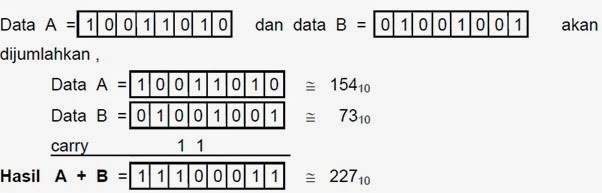
\includegraphics[width=4.14in, height=1.33in, keepaspectratio=false]{1}
\end{center}
\noindent 

\noindent Dalam contoh diatas, telah dilakukan penjumlahan 8 bit tanpa~\textit{carry}, sehingga hasil penjumlahnya masih berupa 8 bit data. Untuk contoh berikutnya akan dilakukan penjumlahan 8 bityang menghasilkan~\textit{carry}.

\noindent \textbf{Contoh :}

\begin{center}
\noindent 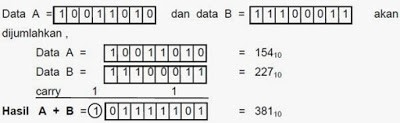
\includegraphics[width=4.17in, height=1.26in, keepaspectratio=false]{2}
\end{center}

\noindent 

\noindent Hasil penjumlahan diatas menjadi 9 bit data, sehingga untuk 8 bit data, hasil penjumlahannya bukan merupakan jumlah 8 bit data A dan B tetapi bit yang e-8 (dihitung mulai dari 0) atau yang disebut~\textit{carry}~juga harus diperhatikan~ sebagai hasil penjumlahan.

\noindent \textbf{3.1.1.2 Penjumlahan Bilangan Oktal}

Proses penjumlahan bilangan oktal sama seperti proses penjumlahan bilangan desimal. Sisa akan timbul / terjadi jika jumlahnya telah melebihi 7 pada setiap tempat.

\noindent \textbf{Contoh :}

\begin{center}
\noindent \includegraphics*[width=4.14in, height=2.08in, keepaspectratio=false]{3}
\end{center}

\noindent 

\noindent \textbf{3.1.1.3 Penjumlahan Bilangan Heksadesimal}

Dalam penjumlahan bilangan heksadesimal, sisa akan terjadi jika jumlah dari setiap tempat melebihi 15.

\begin{center}
\noindent \includegraphics*[width=4.14in, height=1.69in, keepaspectratio=false]{4}~ ~ ~ ~ ~ ~ ~ ~ ~ ~ ~ ~ ~ ~ ~ ~ ~ ~ ~ ~ ~ ~ ~ ~ ~ ~ ~ ~ ~ ~ ~ ~ ~ ~ ~ ~ ~ ~ ~ ~ ~ ~ ~ ~~
\end{center}

\noindent 

\begin{center}
\noindent \includegraphics*[width=3.35in, height=0.91in, keepaspectratio=false]{5}
\end{center}

\noindent 

\noindent \textbf{3.1.2 Pengurangan Bilangan}

\noindent \textbf{3.1.2.1 Pengurangan Bilangan Biner}

Pada pengurangan bilangan biner berlaku aturan seperti di bawah ini,

\begin{center}
\begin{tabular}{|p{0.9in}|p{1.3in}|} \hline 
\textbf{0~ -~ 0} & \textbf{= 0} \\ \hline 
\textbf{0~ -~ 1} & \textbf{= 1 / -1 sebagai~\textit{borrow}} \\ \hline 
\textbf{1~ -~ 0} & \textbf{= 1} \\ \hline 
\textbf{1~ -~ 1} & \textbf{= 0} \\ \hline 
\textbf{0~ -~ 1~ -~ 1} & \textbf{= 0 / - 1 sebagai~\textit{borrow}} \\ \hline 
\textbf{1~ -~ 1~ -~ 1} & \textbf{= 1 / -1 sebagai~\textit{borrow}} \\ \hline 
\end{tabular}
\end{center}

Pada pengurangan jika bilangan yang dikurangi lebih kecil dari pada bilangan pengurangnya maka dilakukan peminjaman (\textit{borrow}) pada tempat yang lebih tinggi.

\noindent \textbf{Contoh :}

\begin{center}
\noindent \includegraphics*[width=4.14in, height=1.33in, keepaspectratio=false]{6}
\end{center}

\noindent 

\noindent \textbf{3.1.2.2 Pengurangan Bilangan Oktal}

Pada pengurangan jika bilangan yang dikurangi lebih kecil dari pada bilangan pengurangnya maka dilakukan peminjaman (\textit{borrow}) pada tempat yang lebih tinggi (dengan nilai 8).

\noindent \textbf{Contoh :}

\noindent \textbf{~}

\begin{center} 
\includegraphics*[width=3.33in, height=1.69in, keepaspectratio=false]{7} 
\end{center}

\textbf{3.1.2.2 Pengurangan Bilangan Heksadesimal}

Pada pengurangan jika bilangan yang dikurangi lebih kecil dari pada bilangan pengurangnya maka dilakukan peminjaman (\textit{borrow}) pada tempat yang lebih tinggi (dengan nilai 16).

\noindent \textbf{Contoh :}

\begin{center}
\noindent \textbf{\includegraphics*[width=3.34in, height=2.08in, keepaspectratio=false]{8}}
\end{center}

\noindent 

\noindent \textbf{3.1.3~\textit{Increment~}dan~\textit{Decrement}}

\textit{Increment~}(bertambah) dan~\textit{Decrement~}(berkurang) adalah dua pengertian yang sering sekali digunakan dalam teknik miroprosessor. Dalam matematik pengertian~\textit{increment}~adalah~\textbf{Bertambah Satu~}dan~\textit{decrement~}artinya~\textbf{Berkurang Satu.}

\noindent \textbf{3.1.3.1~\textit{Increment~}Sistem Bilangan}

Seperti penjelasan diatas bahwa~\textit{increment}~artinya bilangan sebelumnya ditambah dengan 1.

\noindent \textbf{Contoh :}

\begin{center}
\noindent \includegraphics*[width=3.32in, height=2.05in, keepaspectratio=false]{9}
\end{center}

\noindent 

\noindent \textbf{3.1.3.2~\textit{Decrement~}Sistem Bilangan}

\textit{Decrement~}diperoleh dengan cara mengurangi bilangan sebelumnya dengan 1.

\noindent \textbf{Contoh :}

\begin{center}
\noindent \includegraphics*[width=3.33in, height=2.00in, keepaspectratio=false]{10}
\end{center}

\noindent 

\noindent

\section{Komposisi Fungsi}\index{Komposisi Fungsi}

\noindent \textbf{Fungsi}

\noindent Fungsi adalah relasi antara 2 himpunan yang berbeda A dan B yang memasangkan setiap anggota di Himpunan A dengan tepat satu anggota himpunan B.

\begin{center}
\noindent \includegraphics*[width=3.28in, height=1.40in, keepaspectratio=false]{77}
\end{center}

\noindent \textbf{Komposisi Fungsi }

\noindent Komposisi fungsi adalah penggbungan operasi 2 fungsi secara terurut yang nantinya akan meghasilkan sebuah fungsi baru.

\begin{enumerate}
\item  \$(f{\textbackslash}circ g)(x)=f(g(x))\$

\item  \$(g{\textbackslash}circ f)(x)=g(f(x))\$
\end{enumerate}

\noindent 

\noindent \textbf{Sifat Komposisi Fungsi }

\noindent \$(g {\textbackslash}circ f)(x) {\textbackslash}neq (f {\textbackslash}circ g)(x)\$ \$(f{\textbackslash}circ (g{\textbackslash}circ h))(x)=((f{\textbackslash}circ g){\textbackslash}circ h)(x)\$

\noindent Contoh :

\noindent diberikan fungsi :

\begin{enumerate}
\item  \$$\{${\textbackslash}color$\{$Red$\}$ f(x)=2x+1$\}$\$

\item  \$$\{${\textbackslash}color$\{$Blue$\}$ g(x)=3x$\wedge$2$\}$\$

\item  \$$\{${\textbackslash}color$\{$DarkGreen$\}$ h(x)={\textbackslash}frac$\{$1$\}$$\{$x+4$\}$$\}$\$
\end{enumerate}

\noindent 

\begin{enumerate}
\item  \$(f{\textbackslash}circ g)(x)\$ = {\dots}.?
\end{enumerate}

\noindent fungsi \$g(x)\$ disubtitusikan ke fungsi \$f(x)\$

\begin{center}
\noindent \textbf{\includegraphics*[width=2.47in, height=1.14in, keepaspectratio=false]{78}}
\end{center}

\begin{enumerate}
\item \textbf{ }\$(g{\textbackslash}circ h)(x)\$ = {\dots}.?
\end{enumerate}

\noindent fungsi h(x) disubtitusikan ke fungsi g(x)

\begin{enumerate}
\item  \$(h{\textbackslash}circ g{\textbackslash}circ f)(x)\$ ={\dots}?
\end{enumerate}

\noindent fungsi \$f(x)\$ harus disubtitusikan terlebih dahulu ke fungsi \$g(x)\$ , hasilnya nanti akan  baru disubtitusikan ke fungsi \$h(x)\$, perhatikan warna mewakili subtitusi

\begin{center}
\noindent \includegraphics*[width=3.83in, height=2.48in, keepaspectratio=false]{79}
\end{center}

\noindent \textbf{}

\noindent

\section{Fungsi Linear}\index{Fungsi Linear}

\begin{enumerate}
\item \textbf{ Pengertian Fungsi Linier}
\end{enumerate}

\noindent \textbf{}

Fungsi adalah~hubungan matematis antara suatu variabel dengan variabel lainnya.~Unsur-unsurpembentuk fungsi adalah~\textbf{\textit{variabel}},~\textbf{\textit{koefisien}}, dan~\textbf{\textit{konstanta}}.

\textbf{\textit{Variabel}}~adalah unsur yang sifatnya berubah-ubah dari satu keadaan ke keadaan lainnya. Variabel dapat dibedakan menjadi~\textbf{\textit{variabel bebas}}~dan~\textbf{\textit{variabel terikat.}}~\textbf{Variabel bebas}~:variabel yang menjelaskan variabel lainnya.~~Adapun~\textbf{Variabel terikat}~adalah variabel yang diterangkan oleh~\textbf{variabel bebas}

\begin{center}
\includegraphics*[width=4.74in, height=1.51in, keepaspectratio=false]{25}
\end{center}

\textit{Gambar 1 contoh fungsi linier}

\textbf{Koefisien}~adalah bilangan atau angka yang diletakkan tepat di depan suatu variabel, terkait dengan variabel yang bersangkutan.

\begin{center}
\includegraphics*[width=4.85in, height=1.72in, keepaspectratio=false]{26}
\end{center}

\textit{Gambar 2 contoh fungsi linier}



\textbf{Konstanta}~sifatnya tetap dan tidak terkait dengan suatu variabel apapun.



Fungsi linier adalah suatu fungsi yang variabelnya berpangkat satu atau suatu fungsi yang grafiknya merupakan garis lurus. Oleh karena itu fungsi linier sering disebutdengan persamaan garis lurus (pgl) dengan bentuk umumnya sbb.:

\textbf{f : x $\boldsymbol{\mathrm{\to}}$ mx + c} atau \textbf{f(x) = mx + c atau y = mx + c}

m adalah gradien / kemiringan / kecondongan dan c adalah konstanta



\noindent \textbf{Contoh :}Gambarlah grafik y = 5x + 2\textbf{Pertama}~tentukanlah nilai x jika y = 00 = 5x + 2x = -2/5Jadi kordinat yang didapatkan adalah (x,y)yaitu (-2/5 , 0)\textbf{Kedua}~tentukannlah nilai y jika x = 0y = 5x + 2y= 5(0) + 2y +2Jadi kordinat yang didapatkan adalah (x,y) yaitu (0,2)

\noindent Setelah titik potong tercipta teman-teman hanya perlu menarik garis antara kordinat satu dengan kordinat lainnya maka akan jadi seperti ini :

\begin{center}
\noindent \includegraphics*[width=3.06in, height=3.30in, keepaspectratio=false, trim=0.00in 0.00in 3.18in 0.00in]{27}
\end{center}

\textit{Gambar 3 grafik fungsi linier}

\noindent 

\noindent Dari grafik diatas dapat tarik kesimpulan kalau~\textbf{gradien}~itu merupakah~\textbf{arah}~dari garis lurus. Gradien dapat memiliki~\textbf{nilai positif}~jika membentuk garis lurus yang memiliki sudut dengan sumbu x diatas 0 derajat dan kurang dari 90 derajat sebab nilai Tg-nya sudah pasti positive . Gradien dapat memiliki~\textbf{nilai negatif~}jika membentuk garis lurus yang memiliki sudut dengan sumbu x lebih dari 90 derajat dan kurang dari 180derajat sebab nilai Tgnya sudah pasti negatif.Gradien dapat memiliki~\textbf{nilai 0}~jika membentuk garis tegak terhadap sumbu y sehingga membentuk sudut tepat 0 derajat terhadap sumbu x , ini terjadi karena nilai Tg dari 0derajat itu sendiri adalah 0. Gradien dapat memiliki~\textbf{nilai tak berhingga}~jika membentuk garis tegak terhadap sumbu x yang nantinya garis tersebut akan membentuk sudut sebesar 90derajat terhadap sumbu x. Ini terjadi karena nilai Tg 90 derajat adalah tak berhingga.

\noindent Jika membuat persamaan garis lurus yang melalui titik (0,0) dengan gradien sebesar m maka gunakanlah rumus :~\textbf{y = mx}~caranya tinggal masukin nilai m aja kok , nilai m biasanya diketahui di soal .Jika membuat persamaan garis lurus yang memotong sumbu y ditiik (0,n) dan gradiennya diketahui , pakai saja rumus~\textbf{y = mx + n}Jika membuat persamaan garis lurus yang melalui titik A (x1, y1) dan gradiennya diketahui gunakanlah persamaan~\textbf{y-y1 = m (x-x1)}Jika membuat persamaan garis lurus yang melalui dua titik misal titik A(x1,y1) dan B(x2,y2) maka gunakanlah persamaan :

\begin{center}
\noindent \includegraphics*[width=1.80in, height=0.64in, keepaspectratio=false]{28}
\end{center}

\noindent Jika membuat persamaan garis lurus yang memotong sumbu x pada x1 dan sumbu y pada y1 maka cobalah untuk menggunakan rumus :

\noindent 

\begin{center}
\noindent \includegraphics*[width=1.43in, height=0.68in, keepaspectratio=false]{29}
\end{center}

\noindent Untuk yang diatas tadi ini ,yang tetap dirumus hanyalah x dan y saja , sisanya adalah variabel yang ditentukan dalam soal .Nah kalau persamaan garis lurus~\textbf{Ax + By + C = 0}~, nah ini jujur saya benar-benar masih belum mengerti , mungkin kalau ada dari teman-teman yang ingin menjelaskan mohon komentar dibawah.~Nah ini nih temen2 , bener2 sangat berguna dan gak kalah penting .Misalkan ini ada dua garis lurus :Garis lurus~

\noindent ~L${}_{1~}$: y = m${}_{1}$~x + n${}_{1}$~L${}_{2~}$: y = m${}_{2}$~x + n${}_{2~~}$

\noindent 1.) Dua garis lurus berimpit maka m1 = m2 dan n1 = n22.) Dua garis lurus sejajar maka m1 = m2 dan ~n1 tidak sama dengan n23.) Dua garis lurus saling tegak lurus m1 x m2 =-14.) Dua garis lurus saling berpotongan m1 tidak sama dengan m2

\noindent 

\begin{enumerate}
\item  \textbf{Melukis grafik fungsi linier}
\end{enumerate}

\noindent Langkah-langkah melukis grafik fungsi linier

\noindent a Tentukan titik potong dengan sumbu x, y = 0 diperoleh koordinat A( x1, 0)b Tentukan titik potong dengan sumbu y, x = 0 diperoleh koordinat B( 0, y1)c hubungkan dua titik A dan B sehingga terbentuk garis lurusPersamaan linier juga dapat ditulis ditulis dengan simbol y = ax + b (ini untuk memudahkan kita dalam memahami gambar)Jika b bernilai positif : fungsi linier digambarkan garis dari kiri bawah ke kanan atasJika b bernilai negatif : fungsi linier digambarkan garis dari kiri atas ke kanan bawahJika b bernilai nol : digambarkan garis yg sejajar dengan sumbu datar x

\begin{center}
\noindent \includegraphics*[width=3.93in, height=1.68in, keepaspectratio=false]{30}
\end{center}

\noindent ~

\noindent 

\noindent 

\noindent 

\noindent 

\noindent 

\noindent \textit{Gambar 4  Fungsi Linear}

\noindent Apabila b bernilai negatif : Y = 10 - 2X maka kurva bergerak dari kiri atas ke kanan bawah

\begin{center}
\noindent \includegraphics*[width=3.17in, height=2.41in, keepaspectratio=false]{31}
\end{center}

\noindent ~Apabila b bernilai positif : Y = 2 + 2X maka kurva bergerak dari kiri bawah ke kanan atas~~

\begin{center}
\noindent \includegraphics*[width=3.51in, height=2.67in, keepaspectratio=false]{32}
\end{center}

\begin{enumerate}
\item  \textbf{Gradien dan persamaan garis lurus}
\end{enumerate}

\noindent 

\begin{enumerate}
\item  Garis lurus yang melalui titik A(x1, y1) dan B(x2, y2) memiliki gradien m:
\end{enumerate}

\noindent m = y1-y2 atau m = y2-y1x1-x2 x2-x1

\noindent 

\begin{enumerate}
\item  Persamaan garis lurus yang melalui titik A(x1, y1) dan B(x2, y2) adalah:
\end{enumerate}

\noindent y-y1 = x-x1y2-y1 x2-x1

\begin{enumerate}
\item  Persamaan garis lurus (pgl) yang bergradien m dan melalui titik A(x1, y1) adalah:
\end{enumerate}

y = m (x -- x1 ) + y1\textbf{4.  Menentukan gradien dari persamaan garis lurus (pgl)}

\textbf{}

\begin{enumerate}
\item \textbf{ }Persamaan garis lurus : ax + by = c maka gradiennya m = - a/b

\item  Persamaan garis lurus : y = ax + b maka m = a

\item  Garis yang sejajar sumbu x memiliki persamaan y = c dan m = 0

\item  Garis yang sejajar sumbu y memiliki persamaan x = c dan tidak memiliki gradient
\end{enumerate}

\noindent \textbf{5.  Titik potong dua buah garis}

\noindent \textbf{}

\noindent Menentukan titik potong dua buah garis lurus identik dengan menyelesaikanpenyelesaian sistem persamaan linier dua variabel baik dengan metode eleminiasi,metode substitusi maupun metode grafik

\noindent 

\noindent \textbf{6.   Hubungan dua buah garis}

\noindent Dua garis yang bergradien m1 dan m2 dikatakan sejajar jika m1 = m2 dan tegak lurus jika m1 x m2 = -1\textbf{1. Berimpit}

\noindent Dua garis lurus akan berimpit apabila persamaan garis yang satu merupakan kelipatan dari garis yang lain. Dengan demikian , garis~\includegraphics*[width=0.91in, height=0.31in, keepaspectratio=false]{42} akan berimpit dengan garis~\includegraphics*[width=0.99in, height=0.24in, keepaspectratio=false]{43}, jika \includegraphics*[width=2.18in, height=0.23in, keepaspectratio=false]{44}

\begin{center}
\noindent \includegraphics*[width=2.29in, height=1.93in, keepaspectratio=false]{33}\textbf{}
\end{center}

\noindent \textbf{}

\noindent \textbf{2. Sejajar}

\noindent Dua garis lurus akan sejajar apabila lereng/gradien garis yang satu sama dengan lereng/gradien dari garis yang lain. Dengan demikian , garis~\includegraphics*[width=1.06in, height=0.28in, keepaspectratio=false]{45} akan sejajar dengan garis~\includegraphics*[width=0.98in, height=0.24in, keepaspectratio=false]{46}, jika \includegraphics*[width=0.58in, height=0.27in, keepaspectratio=false]{47}

\begin{center}
\noindent \includegraphics*[width=2.27in, height=1.71in, keepaspectratio=false]{34}
\end{center}

\noindent 

\begin{enumerate}
\item  \textbf{Berpotongan}
\end{enumerate}

\noindent Dua garis lurus akan berpotongan apabila lereng/gradien garis yang satu tidak sama dengan lereng/gradien dari garis yang lain. Dengan demikian , garis\includegraphics*[width=0.98in, height=0.26in, keepaspectratio=false]{48}~akan berpotongan dengan garis~\includegraphics*[width=1.02in, height=0.25in, keepaspectratio=false]{49}, jika\includegraphics*[width=0.85in, height=0.34in, keepaspectratio=false]{50}

\begin{center}
\noindent \includegraphics*[width=2.54in, height=1.90in, keepaspectratio=false]{35}
\end{center}

\noindent \textbf{4.   Tegak lurus}

\noindent Dua garis lurus akan saling tegak lurus apabila lereng/gradien garis yang satu merupakan kebalikan dari lereng/gradien dari garis yang lain dengan tanda yang berlawanan. Dengan demikian , garis~\includegraphics*[width=0.98in, height=0.26in, keepaspectratio=false]{51}akan tegak lurus dengan garis~\includegraphics*[width=1.02in, height=0.25in, keepaspectratio=false]{52}, jika atau\includegraphics*[width=0.77in, height=0.34in, keepaspectratio=false]{53}

\begin{center}
\noindent \includegraphics*[width=2.71in, height=2.27in, keepaspectratio=false]{36}
\end{center}

\noindent 

\noindent \textbf{7.  Penggambaran Fungsi Linear}

\textbf{1. Cara Daftar}

\noindent Digunakan untuk melihat perubahan nilai angka dari peubah bebas dab peubah tergantungnya. Contoh :
\noindent y = 2x + 10
\begin{center}
\noindent \includegraphics*[width=6.03in, height=0.73in, keepaspectratio=false]{37}
\end{center}

\noindent 

\noindent 

\begin{center}
\noindent \includegraphics*[width=3.33in, height=2.20in, keepaspectratio=false]{38}
\end{center}

\noindent 

\noindent 

 

~ ~ ~ ~

\noindent 

\noindent \textbf{2. Cara Matematis}

\noindent \textbf{    }

\textbf{   }Dengan cara mencari ciri matematis dari persamaan yang bersangkutan.

     Y = 2x + 10

\noindent Titik potong sumbu y apabila x = 0 maka y = 2 (0) + 10 = 10~~~~~ ~~~~~~~~~~~~~~~~~~~~~~~~~~~~~~~~~~~~~~~~~~~

\noindent 

\noindent Sehingga titik potong pada sumbu y = ( 0,10 )

\noindent 

\noindent Titik potong sumbu x apabila y = 0 maka 0 = 2x + 10

\noindent 

\noindent ~~~~~~~~~~~~~~~~~~~~~~~~~~~~~~~~~~~~~~~~~~~~~~~~~~~~~~~~~    ~- 2x = 10

\noindent ~~~~~~~~~~~~~~~~~~~~~~~~~~~~~~~~~~~~~~~~~~~~~~~~~~~~~~~~~~~~~~~~~~         x = - 5~

\noindent 

\begin{center}
\noindent \includegraphics*[width=3.33in, height=1.88in, keepaspectratio=false]{39}
\end{center}

\noindent sehingga titik potong pada sumbu x = ( -5,0 )

\noindent 

\noindent 

\noindent \textbf{3. ~Mencari fungsi linear}

\noindent \textbf{}

\noindent \textbf{a.~Metode dua titik (dwi koordinat )}

merupakan metode pembentukan persamaan linear ( garis lurus ) dari dua buah titik yang diketahui

\noindent \underbar{( Y -- Y1)~}~~~ =~~\underbar{( X -- X1 )}

\noindent (Y 2 -- Y1)~~~~~ ~(X2 -- X1)

\noindent 

\noindent Contoh buatlah persamaan garis lurus yang melalui titik A (4,2) dan B (2,6)

\noindent 

\noindent Titik A (4,2)~~~~ X1 = 4~~ Y1 = 2

\noindent Titik B (2,6)~~~~ X2 = 2~~~ Y2 = 6

\noindent \underbar{(Y - 2)}~ =~~\underbar{(X - 4)}

\noindent (6 -~ 2)~~~~ ( 2 -- 4) ~ ~ ~ ~ ~

\noindent \underbar{(Y -- 2)~}=~\underbar{(X -- 4) ~~}~

\noindent ~ ~ \eqref{GrindEQ__4_}~~~~~~~~~~ (-2)

\noindent -2y + 4 = 4x -- 16

\noindent ~~~~~ -2y = 4x -- 20

\noindent ~~~~~~~~~y = -2x + 10

\noindent ~

\begin{center}
\noindent \includegraphics*[width=3.33in, height=2.46in, keepaspectratio=false]{40}
\end{center}

\noindent 

\noindent ~ ~ ~ ~ ~ ~ ~ ~ ~ ~ ~ ~ ~ ~ ~ ~ ~ ~ ~ ~ ~ ~ ~ ~ ~ ~ ~ ~ ~ ~ ~ ~ ~ ~ ~ ~ ~ ~ ~ ~ ~ ~ ~ ~ ~ ~ ~ ~~

\noindent ~~~~~~~~~~~~~~~~~~~~~~~~~~~~~~~~~~~~

\noindent \textbf{b.~~~Metode titik potong sumbu}

\noindent \textbf{}

\noindent digunakan untuk kasus tertentu, yaitu jika suatu titik A (x1,y1) merupakan titik potong sumbu Y, misalnya pada titik (0,b) dan titik B (x2,y2) merupakan titik potong sumbu x misalnya pada (a,0) maka persamaan garisnya dapat dibentuk sbb:

\noindent 

\noindent y / b -- 1 = -x / a~~

\noindent y / b + x / a = 1

\noindent 

\noindent \textbf{Contoh :}

\noindent \textbf{}

\noindent apabila diketahui suatu garis dengan titik potong sumbu y adalah (0,6) dan titik potong sumbu x adalah (4,0), carilah persamaan garisnya

\noindent 

\noindent y / b -- 1 = x / a

\noindent y / b + x / a = 1

\noindent y / 6 + x / 4 = 1~~~~~~~~~~~~~~~ x 12

\noindent 12y / 6 + 12x / 4 = 12

\noindent 2y + 3x = 12

\noindent 2y = -3x + 12

\noindent y = -3/2 x + 6

\noindent 

\noindent 

\noindent \textbf{c.~~~Metode kemiringan garis dan titik}

\noindent Apabila diketahui suatu titik A (x1,y1) dan dilalui oleh suatu garis lurus yang memiliki kemiringan m, maka persamaannya adalah :

\noindent 

\noindent y -- y1 = m (x -- x1) persamaan garis yang melalui titik (x1,y1) dengan kemiringan sebesar m. 

\noindent \textbf{}

\noindent \textbf{Contoh:}

\noindent \textbf{}

\noindent carilah persamaan garis yang melalui suatu titik (4,2) dan kemiringan -3

\noindent 

\noindent y -- y1 = m(x -- x1)

\noindent y -- 2~~ = -3(x -- 4 )

\noindent ~~~~~~~~~~ = -3x + 12

\noindent ~~~~~~ y~ = -3x + 14

\noindent 

\noindent \textbf{d.~~~~~Metode kemiringan garis dan titik potong sumbu}

\noindent Apabila diketahui suatu titik yang berkoordinat (0,b) merupakan titik potong dengan sumbu y sebuah garis lurus yang memiliki kemiringan garis m, maka persamaan garis tersbut adalah y = mx + b, merupakan persamaan garis yang melalui titik potong sumbu y dengan kemiringan m, 

\noindent 

\noindent \textbf{Contoh :}

\noindent \textbf{}

\noindent Apabila suatu garis memiliki titik potong dengan sumbu y pada (0,-4) dan kemiringannya 5 maka bagaimana persamaan garisnya :

\noindent 

\noindent y = mx + b

\noindent y = 5x -- 4

\noindent 

\noindent \eject Contoh soal persamaan linier

\begin{enumerate}
\item  Suatu fungsi linear ditentukan oleh y = 4x -- 2 dengan daerah asal $\{$x {\textbackslash}-1    x    2, x    R$\}$.

\item  Buat tabel titik-titik yangmemenuhi persamaan diatas .

\item  Tentukan titik potong grafik dengan sumbu X dan sumbu Y.
\end{enumerate}

\noindent Penyelesaian :

\begin{enumerate}
\item \begin{enumerate}
\item  \textbf{Ambil sembarang titik pada domain}
\end{enumerate}
\end{enumerate}

\noindent 

 X -1 0 1 2W3956W5012W6151W7290W8429 Y= 4x-2 -6 -2 2 6W3956W5012W6151W7290W8429

\begin{enumerate}
\item  \textbf{Titik potong dengan sumbu x ( y= 0 )}
\end{enumerate}

\noindent \textbf{}

\noindent y = 4x -- 2

\noindent 0 = 4x - 2

\noindent 2 = 4x

\noindent x =  1/2

\noindent Jadi titik potong dengan sumbu X adalah ( ½,0)

\noindent 

\begin{enumerate}
\item  \textbf{Titik potong dengan sumbu Y ( x = 0 )}
\end{enumerate}

\noindent y = 4x -- 2

\noindent y = 4(0) -- 2

\noindent y = -2

\noindent Jadi titik potong dengan sumbu Y adalah (0,-2)

\noindent 

\noindent 

\noindent

\section{Fungsi Kuadrat}\index{Fungsi Kuadrat}

\noindent Fungsi kuadrat (\textit{quadratic function}) adalah fungsi polinomial yang berderajat dua. Bentuk umum dari fungsi kuadrat adalah~\textit{f}(\textit{x}) =~\textit{ax}${}^{2}$~+~\textit{bx}~+~\textit{c},~\textit{a}~$\mathrm{\neq}$ 0. Fungsi kuadrat dapat memotong sumbu-\textit{x}~2 kali, 1 kali, atau tidak memotong sumbu-\textit{x}~sama sekali.

\begin{center}
\noindent \includegraphics*[width=6.25in, height=4.17in, keepaspectratio=false]{54}
\end{center}

\noindent Pada buku ini akan dibahas fungsi kuadrat yang memotong sumbu-\textit{x}~minimal di satu titik, misalkan di titik-titik (\textit{x}${}_{1}$, 0) dan (\textit{x}${}_{2}$, 0). Sehingga didapatkan f(\textit{x}${}_{1}$) = f(\textit{x}${}_{2}$) = 0. Apabila fungsi kuadrat yang memotong sumbu-\textit{x}~di dua titik tersebut melalui titik (\textit{x}${}_{3}$,~\textit{y}${}_{3}$), maka fungsi kuadrat tersebut dapat ditentukan bentuknya, yaitu sebagai berikut:

\begin{center}
\noindent \includegraphics*[width=2.87in, height=0.76in, keepaspectratio=false]{55}
\end{center}

\noindent \textbf{CONTOH SOAL}

\noindent Susunlah fungsi kuadrat yang memotong sumbu-\textit{x}~di titik (2, 0) dan titik (--1, 0) serta melalui titik (3, 12)!

\noindent \textbf{Jawab:}Karena fungsi kuadrat yang dimaksud melalui titik (3, 12) serta memotong sumbu-\textit{x}~di titik (2, 0) dan titik (--1, 0), maka kita cukup mensubstitusikan 3 pada~\textit{x}, 12 pada~\textit{f}(\textit{x}), serta absis-absis titik potong sumbu-\textit{x}~pada~\textit{x}${}_{1}$~dan~\textit{x}${}_{2}$. Sehingga,

\begin{center}
\noindent \includegraphics*[width=6.50in, height=2.21in, keepaspectratio=false]{56}
\end{center}

\noindent Setelah diperoleh~\textit{a}~= 3, substitusikan~\textit{a}~tersebut pada rumus dengan membiarkan~\textit{x}~dan~\textit{f}(\textit{x}).

\begin{center}
\noindent \includegraphics*[width=6.50in, height=2.21in, keepaspectratio=false]{57}
\end{center}

\noindent Sehingga diperoleh fungsi kuadrat yang dimaksud adalah~\textit{f}(\textit{x}) = 3\textit{x}${}^{2}$~-- 3\textit{x}~-- 6. Untuk menguji hasil yang diperoleh, mari kita uji fungsi tersebut apakah melalui titi-titik (2, 0), (--1, 0), dan (3, 12).

\begin{center}
\noindent \includegraphics*[width=6.50in, height=2.21in, keepaspectratio=false]{58}
\end{center}

\noindent Sehingga fungsi kuadrat yang diperoleh memenuhi permintaan soal. Untuk menguji kompetensi mengenai materi ini silahkan kerjakan soal berikut.

\noindent \textbf{SOAL LATIHAN}

\noindent Perhatikan gambar di bawah!

\begin{center}
\noindent \includegraphics*[width=6.25in, height=4.17in, keepaspectratio=false]{59}
\end{center}

\noindent Tentukanlah fungsi kuadrat yang grafiknya digambarkan seperti gambar di atas!

Fungsi kuadrat memiliki grafik yang berbentuk parabola yang terbuka ke atas atau ke bawah. Sehingga fungsi kuadrat dapat memiliki nilai minimum ataupun maksimum, tergantung dari koefisien~\textit{x}${}^{2}$~(\textit{a}) fungsi kuadrat tersebut. Apabila nilai~\textit{a}~positif, maka fungsi kuadrat tersebut memiliki nilai minimum. Sedangkan apabila nilai~\textit{a}~negatif, fungsi kuadrat tersebut memiliki nilai maksimum. Titik di mana nilai maksimum/minimum dari fungsi kuadrat tersebut disebut~\textbf{titik ekstrim}, disimbolkan (\textit{x}${}_{p}$,~\textit{y}${}_{p}$).

\noindent Fungsi kuadrat yang memiliki titik ekstrim (\textit{x}${}_{p}$,~\textit{y}${}_{p}$) dan melalui satu titik lain dapat disusun dengan menggunakan rumus berikut:

\begin{center}
\noindent \includegraphics*[width=2.52in, height=0.83in, keepaspectratio=false]{60}
\end{center}

\noindent Untuk lebih memahami mengenai topik menyusun fungsi kuadrat apabila diketahui titik ekstrim dan satu titik lain yang dilaluinya, perhatikan contoh soal berikut.

\noindent \textbf{CONTOH SOAL}

\noindent Susunlah fungsi kuadrat yang memiliki titik ekstrim di (2, --5) dan melalui titik (1, 4)!

\noindent \textbf{Jawab:}Fungsi kuadrat yang memiliki titik ekstrim di (2, --5) dan melalui titik (1, 4) dapat ditentukan sebagai berikut:

\begin{center}
\noindent \includegraphics*[width=5.81in, height=1.56in, keepaspectratio=false]{61}
\end{center}

\noindent Untuk~\textit{a}~= 9, diperoleh

\begin{center}
\noindent \includegraphics*[width=5.09in, height=1.57in, keepaspectratio=false]{62}
\end{center}

\noindent Jadi, fungsi kuadrat yang memiliki titik ekstrim (2, --5) dan melalui titik (1, 4) adalah~\textit{y}~= 9\textit{x}${}^{2}$~-- 36\textit{x}~+ 31

\noindent \eject 

Pada umumnya, dalam menyusun fungsi kuadrat diperlukan minimal tiga titik yang dilaluinya. Hal ini tidak berlaku untuk titik ekstrim. Apabila diketahui titik ekstrim suatu fungsi kuadrat, maka diperlukan satu titik lagi (total dua titik) untuk menyusun fungsi fungsi kuadrat tersebut. Yang akan dibicarakan di sini adalah menyusun fungsi kuadrat jika diketahui ketiga titik yang dilaluinya, titik ekstrim tidak masuk dalam ketiga titik tersebut.

\noindent Untuk menyusun fungsi kuadrat jika diketahui ketiga titik yang dilaluinya digunakan bentuk umum dari fungsi kuadrat berikut:

\begin{center}
\noindent \includegraphics*[width=2.01in, height=0.72in, keepaspectratio=false]{63}
\end{center}

\noindent Dengan~\textit{a},~\textit{b}, dan~\textit{c}~bilangan real, serta~\textit{a}~$\mathrm{\neq}$ 0.

\noindent Untuk mengetahui bagaimana menyusun fungsi kuadrat jika diketahui ketiga titik yang dilaluinya, perhatikan contoh soal berikut.

\noindent \textbf{CONTOH SOAL}

\noindent Tentukan fungsi kuadrat yang melalui titik-titik (--1, 6) dan (2, 12) serta memotong sumbu-\textit{y}~pada~\textit{y}~= 2!

\noindent \textbf{Jawab}Fungsi kuadrat yang akan dicari memotong sumbu-\textit{y}~pada~\textit{y}~= 2, atau dengan kata lain memotong sumbu-\textit{y}~di titik (0, 2). Sehingga,

\begin{center}
\noindent \includegraphics*[width=4.25in, height=1.90in, keepaspectratio=false]{64}
\end{center}

\noindent Setelah itu kita substitusikan titik (--1, 6) pada persamaan.

\begin{center}
\noindent \includegraphics*[width=5.44in, height=2.25in, keepaspectratio=false]{65}
\end{center}

\noindent Persamaan yang diperoleh ini dimisalkan dengan~\textbf{persamaan 1}.

\noindent Lanjut ke titik (2, 12). Apabila titik (2, 12) disubstitusikan ke bentuk umum fungsi kuadrat, akan menjadi seperti berikut.

\begin{center}
\noindent \includegraphics*[width=5.26in, height=2.46in, keepaspectratio=false]{66}
\end{center}

\noindent Persamaan yang diperoleh ini dimisalkan dengan~\textbf{persamaan 2}.

\noindent Selanjutnya, lakukan~\textbf{metode eliminasi}~persamaan 2 terhadap persamaan 1 dengan menghilangkan/mengeliminasi variabel~\textit{b}.

\begin{center}
\noindent \includegraphics*[width=2.28in, height=1.68in, keepaspectratio=false]{67}
\end{center}

\noindent Sehingga diperoleh~\textit{a}~= 3. Substitusikan hasil ini ke persamaan 1 atau 2. Apabila~\textit{a}~= 3 disubstitusikan ke persamaan 1, maka 3 --~\textit{b}~= 4. Diperoleh~\textit{b}~= 3 -- 4 = --1. Jadi, fungsi kuadrat yang melalui titik-titik (--1, 6) dan (2, 12) serta memotong sumbu-\textit{y}~pada~\textit{y}~= 2 adalah~\textit{f}(\textit{x}) = 3\textit{x}${}^{2}$~--~\textit{x}~+ 2.

\noindent \textit{Fungsi kuadrat yang melalui titik-titik (--1, 6) dan (2, 12) serta memotong sumbu-y pada  y = 2 adalah f(x) = 3x${}^{2}$~-- x + 2.}

\noindent Untuk meyakinkan akan kebenaran jawaban ini, mari kita uji fungsi kuadrat ini dengan titik-titik (--1, 6), (2, 12), dan (0, 2).

\begin{center}
\noindent \includegraphics*[width=4.28in, height=4.82in, keepaspectratio=false]{68}
\end{center}

\noindent Pada perhitungan di atas dapat diperoleh bahwa untuk~\textit{x}~= --1 diperoleh~\textit{y}~= 6, untuk~\textit{x}~= 2 diperoleh~\textit{y}~= 12, dan untuk~\textit{x}~= 0 diperoleh~\textit{y}~= 2. Sehingga fungsi~\textit{f}(\textit{x}) = 3\textit{x}${}^{2}$~--~\textit{x}~+ 2 memotong titik-titik (--1, 6), (2, 12), dan (0, 2). Sesuai yang diminta soal. Jadi, dari hasil ini dapat disimpulkan bahwa pekerjaan kita dalam menyusun fungsi kuadrat di atas benar.

\noindent \textbf{Grafik Fungsi Kuadrat}

\noindent Fungsi kuadrat merupakan suatu fungsi yang memiliki satu variabel yang pangkat tertingginya adalah 2. Fungsi kuadrat memiliki bentuk umum~\textit{f}(\textit{x}) =~\textit{ax}${}^{2}$~+~\textit{bx}~+~\textit{c}, dengan~\textit{a},~\textit{b},~\textit{c}~bilangan real dan~\textit{a}~$\mathrm{\neq}$ 0. Pada pembahasan ini akan ditunjukkan bagaimana cara melukis grafik fungsi kuadrat, khususnya grafik fungsi~\textit{f}(\textit{x}) =~\textit{x}${}^{2}$~dan~\textit{f}(\textit{x}) = --\textit{x}${}^{2}$. Mengapa memilih fungsi-fungsi kuadrat tersebut? Karena fungsi-fungsi tersebut merupakan fungsi-fungsi kuadrat yang paling sederhana.

\noindent \textbf{Melukis Grafik Fungsi~\textit{f}(\textit{x}) =~\textit{x}${}^{2}$}

\noindent Sebelum melukis grafik fungsi~\textit{f}(\textit{x}) =~\textit{x}${}^{2}$, perlu diketahui bahwa semua fungsi kuadrat merupakan fungsi kontinu. Sehingga apabila dilukiskan grafik fungsinya, akan terbentuk grafik fungsi yang halus. Selain itu, fungsi~\textit{f}(\textit{x}) =~\textit{x}${}^{2}$~merupakan fungsi genap, yaitu fungsi yang nilai~\textit{f}(\textit{x}) =~\textit{f}(--\textit{x}). Grafik dari fungsi genap memiliki sumbu simetri pada sumbu-\textit{y}. Berikut ini langkah-langkah dalam melukis grafik fungsi~\textit{f}(\textit{x}) =~\textit{x}${}^{2}$.

\begin{enumerate}
\item  Cacahlah titik-titik yang dilalui oleh grafik fungsi~\textit{f}(\textit{x}) =~\textit{x}${}^{2}$. Karena grafik fungsi tersebut memiliki sumbu simetri pada sumbu-\textit{y}, pilihlah~\textit{x}~= -- 3, -- 2, -- 1, 0, 1, 2, 3.\textbf{}
\end{enumerate}

\begin{center}
\noindent \includegraphics*[width=6.25in, height=1.56in, keepaspectratio=false]{69}\textbf{}
\end{center}

\noindent \textbf{}

\noindent \textbf{}

\noindent \textbf{}

\noindent \textbf{}

\noindent \textbf{}

\noindent \textbf{}

\noindent \textbf{}

\begin{enumerate}
\item \textbf{ }Lukislah titik-titik dengan koordinat (\textit{x},~\textit{f}(\textit{x})) pada koordinat Cartesius.\textbf{}
\end{enumerate}

\begin{center}
\noindent \includegraphics*[width=5.50in, height=3.67in, keepaspectratio=false]{70}\textbf{}
\end{center}

\begin{enumerate}
\item \textbf{ }Hubungkan titik-titik tersebut dengan menggunakan kurva halus. Grafik yang terbentuk merupakan grafik fungsi~\textit{f}(\textit{x}) =~\textit{x}${}^{2}$.\textbf{}
\end{enumerate}

\begin{center}
\noindent \includegraphics*[width=5.25in, height=3.50in, keepaspectratio=false]{71}\textbf{}
\end{center}

Pada~pembahasan sebelumnya~telah dibahas mengenai 2 grafik fungsi kuadrat yang paling sederhana, yaitu grafik~\textit{f}(\textit{x}) =~\textit{x}${}^{2}$~dan~\textit{f}(\textit{x}) = --~\textit{x}${}^{2}$. Bagaimana dengan grafik-grafik fungsi kuadrat lainnya? Seperti diketahui, bentuk umum dari fungsi kuadrat adalah~\textit{f}(\textit{x}) =~\textit{ax}${}^{2}$~+~\textit{bx}~+~\textit{c}.~\textbf{Pada pembahasan ini akan ditunjukkan cara melukis grafik fungsi kuadrat yang memiliki nilai~\textit{a}~= 1 (\textit{f}(\textit{x}) =~\textit{x}${}^{2}$~+~\textit{bx}~+~\textit{c})}. Dalam melukis grafik fungsi kuadrat dengan~\textit{a}~= 1 dapat digunakan proses transformasi grafik fungsi~\textit{f}(\textit{x}) =~\textit{x}${}^{2}$. Berikut ini beberapa jenis grafik fungsi kuadrat yang merupakan hasil transformasi dari grafik fungsi~\textit{f}(\textit{x}) =~\textit{x}${}^{2}$.

\noindent \textbf{Grafik Fungsi~\textit{f}(\textit{x}) = (\textit{x}~--~\textit{p})${}^{2}$}

\noindent Grafik fungsi~\textit{f}(\textit{x}) = (\textit{x}~--~\textit{p})${}^{2}$,~\textit{p}~bilangan real positif, merupakan hasil pergeseran/translasi grafik~\textit{f}(\textit{x}) =~\textit{x}${}^{2}$~\textbf{ke kanan}~sejauh~\textit{a}. Apabila fungsi~\textit{f}(\textit{x}) =~\textit{x}${}^{2}$~memiliki sumbu simetri pada sumbu-\textit{y}, maka fungsi~\textit{f}(\textit{x}) = (\textit{x}~--~\textit{a})${}^{2}$~memiliki sumbu simetri pada garis~\textit{x}~=~\textit{a}. Misalkan untuk fungsi~\textit{f}(\textit{x}) = (\textit{x}~-- 2)${}^{2}$~=~\textit{x}${}^{2}$~-- 4\textit{x}~+ 4. Grafik ini merupakan hasil translasi grafik~\textit{f}(\textit{x}) =~\textit{x}${}^{2}$~ke kanan sejauh 2 satuan sehingga sumbu simetrinya adalah~\textit{x}~= 2. Perhatikan gambar berikut:

\begin{center}
\noindent \includegraphics*[width=6.25in, height=4.17in, keepaspectratio=false]{72}\textbf{}
\end{center}

\noindent Sedangkan grafik fungsi~\textit{f}(\textit{x}) = (\textit{x}~+~\textit{p})${}^{2}$~merupakan hasil pergeseran grafik fungsi~\textit{f}(\textit{x}) =~\textit{x}${}^{2}$ ${}^{ }$\textbf{ke kiri}~sejauh~\textit{p}~satuan.

\noindent \textbf{Grafik Fungsi~\textit{f}(\textit{x}) =~\textit{x}${}^{2}$~+~\textit{q}}

\noindent 

\noindent Grafik fungsi~\textit{f}(\textit{x}) =~\textit{x}${}^{2}$~+~\textit{q},~\textit{q}~bilangan real positif, merupakan hasil translasi grafik~\textit{f}(\textit{x}) =~\textit{x}${}^{2}$\textbf{ke atas}~sejauh~\textit{q}~satuan. Misalkan~\textit{f}(\textit{x}) =~\textit{x}${}^{2}$~+ 3. Grafik dari fungsi tersebut merupakan hasil translasi dari grafik~\textit{f}(\textit{x}) =~\textit{x}${}^{2}$~ke atas sejauh 3 satuan. Perhatikan gambar berikut.

\noindent 

\begin{center}
\noindent \includegraphics*[width=6.25in, height=4.17in, keepaspectratio=false]{73}\textbf{}
\end{center}

\noindent Sedangkan grafik fungsi~\textit{f}(\textit{x}) =~\textit{x}${}^{2}$~--~\textit{q~}merupakan hasil translasi grafik~\textit{f}(\textit{x}) =~\textit{x}${}^{2}$~\textbf{ke bawah }sejauh~\textit{q}~satuan.

\noindent \eject 

\noindent Pembahasan selanjutnya ini akan ditunjukkan bagaimana~\textbf{melukis grafik fungsi kuadrat yang berbentuk \textit{f}(\textit{x}) =~\textit{ax}${}^{2}$~+~\textit{bx}~+~\textit{c}}, dengan~\textit{a}~bilangan real bukan nol (\textit{a}~$\mathrm{\neq}$ 0) dan bukan satu (\textit{a}~$\mathrm{\neq}$ 1).

\noindent Sebelum membahas bagaimana melukis grafik fungsi kuadrat yang dimaksud, akan dibahas mengenai topik~\textbf{melengkapkan kuadrat}. Bentuk fungsi kuadrat~\textit{f}(\textit{x}) =~\textit{ax}${}^{2}$~+~\textit{bx}+~\textit{c}~dapat diubah bentuknya menjadi bentuk lain, dengan teknik melengkapkan kuadrat. Perhatikan gambar di bawah ini.

\begin{center}
\noindent \includegraphics*[width=5.73in, height=5.73in, keepaspectratio=false]{74}\textbf{}
\end{center}

\noindent Dari fungsi di atas dapat diketahui dengan mudah bahwa fungsi tersebut memiliki titik ekstrim, (\textit{x${}_{p}$},~\textit{y${}_{p}$}). Titik ekstrim dapat berupa nilai maksimum ataupun maksimum suatu fungsi kuadrat tersebut, tergantung nilai~\textit{a}. Apabila~\textit{a}~positif maka titik tersebut adalah nilai minimum, apabila~\textit{a}~negatif maka titik tersebut merupakan nilai maksimum. Titik ekstrim dapat ditentukan apabila yang dikuadratkan pada fungsi kuadrat di atas (setelah diubah dengan melengkapkan kuadrat) adalah nol. Mengapa? Karena bentuk kuadrat memiliki nilai minimum nol.

\begin{center}
\noindent \includegraphics*[width=4.43in, height=1.30in, keepaspectratio=false]{75}\textbf{}
\end{center}

\noindent \textbf{Grafik Fungsi Kuadrat~\textit{f}(\textit{x}) =~\textit{ax}${}^{2}$~+~\textit{bx}~+~\textit{c}.}

\noindent Untuk melukis grafik fungsi kuadrat~\textit{f}(\textit{x}) =~\textit{ax}${}^{2}$~+~\textit{bx}~+~\textit{c}, terlebih dahulu cari titik ekstrimnya kemudian cari 2 titik lainnya yang letaknya di kanan dan kiri titik ekstrim tersebut. Setelah itu, plot ketiga titik tersebut pada koordinat Cartesius dan hubungkan dengan kurva halus. Misalkan akan dilukis grafik fungsi~\textit{f}(\textit{x}) = 2\textit{x}${}^{2}$~--12\textit{x}~+ 17. Grafik fungsi tersebut memiliki nilai~\textit{a}~= 2,~\textit{b}~= -- 12, dan~\textit{c}~= 17. Sehingga titik ekstrimnya adalah (3, --1). Dengan substitusi~\textit{x}~= 0 dan~\textit{x}~= 6 ke fungsi kuadrat tersebut diperoleh 2 titik lainnya adalah (0, 17) dan (6, 17). Berikut adalah grafik dari fungsi~\textit{f}(\textit{x}) = 2\textit{x}${}^{2}$~--12\textit{x}~+ 17.

\begin{center}
\noindent \includegraphics*[width=3in, height=3in, keepaspectratio=false, trim=0.33in 0.00in 0.28in 0.08in]{76}\textbf{}
\end{center}

\noindent

\section{Fungsi Inversi}\index{Fungsi Inversi}

\noindent Pengertian Invers

  Invers suatu fungsi tidak selalu merupakan fungsi. Jika invers suatu fungsi merupakan fungsi maka invers fungsi itu disebut fungsi invers. Misalkan \textit{f} fungsi dari himpunan A ke B yang dinyatakan dengan diagram panah sbb:

\noindent 

\begin{center}
\noindent \includegraphics*[width=2.49in, height=1.78in, keepaspectratio=false]{80}
\end{center}

\noindent sehingga diperoleh himpunan pasangan berurutan:

\noindent $f:\{ (a,b)|a\in A$ dan $b\in B\} $

\noindent 

Kalau diadakan pengubahan domain menjadi kodomain dan kodomain menjadi domaian, maka diagram panahnya menjadi

\begin{center}
\noindent \includegraphics*[width=2.18in, height=1.59in, keepaspectratio=false]{81}
\end{center}

dan himpunan pasangan berurutannya menjadi $\{ (b,a)|b\in B$ dan $a\in A\} $.

\noindent Relasi yang diperoleh dengan cara seperti di atas disebut invers fungsi f dan dilambangkan dengan $f^{-1} $

\noindent 

\noindent Definisi:

\noindent Jika fungsi $f:A\to B$dinyatakan dengan pasangan berurutan $f:\{ (a,b)|a\in A$ dan $b\in B\} $maka invers fungsi f adalah $f^{-1} :B\to A$ ditentukan oleh $f^{-1} =\{ (b,a)|b\in B$ dan $a\in A\} $

\noindent 

\begin{center}
\noindent \includegraphics*[width=2.46in, height=2.11in, keepaspectratio=false]{82}
\end{center}

\begin{center}
\includegraphics*[width=2.39in, height=2.22in, keepaspectratio=false]{83}
\end{center}

\begin{enumerate}
\item  \eqref{GrindEQ__2_}
\end{enumerate}

\noindent 

\noindent 

\begin{center}
\noindent \includegraphics*[width=2.14in, height=1.92in, keepaspectratio=false]{84}
\end{center}

\noindent \eqref{GrindEQ__3_}

\noindent 

Tampak bahwa yang inversnya juga merupakan fungsi hanya pada gambar \eqref{GrindEQ__3_}. Jika invers suatu fungsi merupakan fungsi, maka invers fungsi itu disebut fungsi invers.

\noindent \textbf{}

\begin{enumerate}
\item \begin{enumerate}
\item \textbf{ Syarat-syarat Invers }
\end{enumerate}
\end{enumerate}

Dalam fungsi ini invers mempunyai syarat-syarat khusus invers, diantaranya sebagai berikut :\textbf{}

\begin{tabular}{|p{3.1in}|} \hline 
\textbf{FUNGSI INVERS} \\ \hline 
f${}^{-1}$(x) = (x-b)/a ; a ? 0 \\ \hline 
f${}^{-1}$(x) = (-dx+b)/(cx-a) ; x ? a/c \\ \hline 
f${}^{-1}$(x) = (-b+?(b²-4a(c-x))/2a ; a ? 0 \\ \hline 
f${}^{-1}$(x) = a${}^{x}$/c ; c ? 0 \\ \hline 
f${}^{-1}$(x) =${}^{ a}$log x${}^{1/c}$ = 1/c ${}^{a}$log x ; c?0 \\ \hline 
f${}^{-1}$(x) =${}^{ a}$log x${}^{1/c}$ = 1/c ${}^{a}$log x ; c?0 \\ \hline 
\end{tabular}

Keterangan : \textit{fungsi invers ini ada, jika syarat-syaratnya terpenuhi}

\noindent 

\noindent Fungsi kuadrat secara umum tidak mempunyai invers, tetapi dapat mempunyai invers jika daerah definisinya dibatasi.

\noindent 

\begin{center}
\noindent \includegraphics*[width=4.69in, height=1.16in, keepaspectratio=false]{85}
\end{center}

\noindent 

\noindent 

\noindent f(x) = x² untuk X $>$ 0 f${}^{-1}$(x) = x untuk X $>$ 0

\noindent 

\begin{enumerate}
\item \begin{enumerate}
\item  \textbf{Menentukan Rumus Fungsi Invers}
\end{enumerate}
\end{enumerate}

Beberapa langkah untuk menentukan rumus fungsi invers f${}^{-1}$(x) jika f (x) diketahui adalah sebagai berikut :\textbf{}


\paragraph{ Ubah persamaan y = f (x) dalam bentuk f sebagai fungsi y.}


\paragraph{ Bentuk x sebagai fungsi y pada langkah 1 dinamai dengan f${}^{-1}$(y).}


\paragraph{ Ganti y pada f${}^{-1}$(y) dengan x untuk memperoleh f${}^{-1}$(x). Maka f${}^{-1}$(x) adalah rumus fungsi invers fungsi f (x).}

\noindent \textbf{}

\noindent        Perhatikan diagram panah berikut :

\begin{center}
\noindent \includegraphics*[width=2.78in, height=1.61in, keepaspectratio=false]{86}
\end{center}

\noindent 

\noindent 

y adalah peta dari x oleh fungsi f, sehingga pemetaan oleh fungsi f dapat dinayatakan dengan persamaan:
\[y=f(x)\] 


Kalau f${}^{-1}$ adalah invers dari fungsi f maka x adalah peta dari y oleh fungsi f${}^{-1}$ sehingga diperoleh persamaan:

\noindent 
\[x=f^{-1} (y)\] 


Selanjutnya peubah x diganti dengan y dan peubah y diganti dengan x. \textbf{}

\noindent 

\begin{enumerate}
\item  \textbf{Penyelesaian Masalah}
\end{enumerate}

\noindent Langkah ke-1

\begin{enumerate}
\item  Melengkapi tabel fungsi y = f(x)
\end{enumerate}

\noindent Misalkan fungsi \textit{f} dari \textit{x} ke \textit{y} didefinisikan sebagai \textit{y} = \textit{f} \textit{x}), seperti Tabel 62.1. Salin dan lengkapilah Tabel 2.1. Tabel 2.1\textbf{ }Fungsi\textbf{ }\textit{y}\textbf{ }=\textbf{ }\textit{f}\textbf{ }\textit{x})

\noindent 

\noindent Tabel 2.1

\noindent 

\begin{tabular}{|p{0.6in}|p{0.4in}|p{0.3in}|p{0.2in}|p{0.2in}|p{0.2in}|p{0.2in}|p{0.2in}|p{0.2in}|p{0.2in}|p{0.2in}|} \hline 
\textit{x}  & 0 & 1 & 2 & 3 & 4 & 5 & 6 & 7 & 8 \\ \hline 
 (masukan) &  &  &  &  &  &  &  &  &  \\ \hline 
 &  &  &  &  &  &  &  &  &  &  \\ \hline 
\textit{y}  & 0 & 2 & 4 & 6 & 8 & .. & .. & . & . \\ \hline 
 (keluaran) &  &  &  &  &  &  &  &  &  \\ \hline 
 &  &  &  &  &  &  &  &  &  &  \\ \hline 
\end{tabular}



\begin{enumerate}
\item  Menukarkan nilai-nilai masukan dan keluaran
\end{enumerate}

\noindent Tukarkan nilai-nilai masukan dan keluaran tersebut seperti Tabel 2.2, kemudian salin dan lengkapilah Tabel 2.2 

\noindent \textbf{}

\noindent Tabel 2.2

\noindent 

\begin{tabular}{|p{0.6in}|p{0.4in}|p{0.3in}|p{0.2in}|p{0.2in}|p{0.2in}|p{0.2in}|p{0.2in}|p{0.2in}|p{0.2in}|p{0.2in}|} \hline 
\textit{y}  & 0 & 2 & 4 & 6 & 8 &  &  &  &  \\ \hline 
 (masukan) &  &  &  &  &  &  &  &  &  \\ \hline 
 &  &  &  &  &  &  &  &  &  &  \\ \hline 
\textit{x}  & 0 & 1 & 2 & 3 & 4 & 5 & 6 & 7 & 8 \\ \hline 
 (keluaran) &  &  &  &  &  &  &  &  &  \\ \hline 
 &  &  &  &  &  &  &  &  &  &  \\ \hline 
\end{tabular}



\noindent 

\noindent 

\noindent Langkah ke-2

\noindent 

\noindent 

\begin{enumerate}
\item  Melengkapi tabel fungsi s = g(r)
\end{enumerate}

\noindent Misalkan fungsi \textit{g} dari \textit{r} ke \textit{s} didefinisikan sebagai \textit{s} = \textit{g}(\textit{r}), seperti Tabel 2.3. Salin dan lengkapilah Tabel 2.3. Tabel 2.3\textbf{ }Fungsi\textbf{ }\textit{s}\textbf{ }=\textbf{ }\textit{g}(\textit{r})

\noindent Tabel 2.3

\noindent 

\begin{tabular}{|p{0.6in}|p{0.4in}|p{0.3in}|p{0.2in}|p{0.2in}|p{0.2in}|p{0.2in}|p{0.2in}|p{0.2in}|p{0.2in}|p{0.2in}|} \hline 
\textit{r}  & -4 & -3 & -2 & -1 & 0 & 1 & 2 & 3 & 4 \\ \hline 
 (masukan) &  &  &  &  &  &  &  &  &  \\ \hline 
 &  &  &  &  &  &  &  &  &  &  \\ \hline 
\textit{s}  & . & 9 & 4 & 1 & 0 & 1 & 4 & 9 & . \\ \hline 
 (keluaran) &  &  &  &  &  &  &  &  &  \\ \hline 
 &  &  &  &  &  &  &  &  &  &  \\ \hline 
\end{tabular}



\begin{enumerate}
\item  Menukarkan nilai-nilai masukan dan keluaran
\end{enumerate}

\noindent Tukarkan nilai-nilai masukan dan keluaran tersebut seperti Tabel 2.2, lalu salin dan lengkapi Tabel 2.4.

\noindent \textbf{}

\noindent Tabel 2.4

\noindent 

\begin{tabular}{|p{0.6in}|p{0.4in}|p{0.3in}|p{0.2in}|p{0.2in}|p{0.2in}|p{0.2in}|p{0.2in}|p{0.2in}|p{0.2in}|p{0.2in}|} \hline 
\textit{s}  &  & 9 & 4 & 1 & 0 & 1 & 4 & 9 &  \\ \hline 
 (masukan) &  &  &  &  &  &  &  &  &  \\ \hline 
 &  &  &  &  &  &  &  &  &  &  \\ \hline 
\textit{r}  & --4 & --3 & --2 & --1 & 0 & 1 & 2 & 3 & 4 \\ \hline 
 (keluaran) &  &  &  &  &  &  &  &  &  \\ \hline 
 &  &  &  &  &  &  &  &  &  &  \\ \hline 
 &  &  &  &  &  &  &  &  &  &  \\ \hline 
\end{tabular}



\noindent 

\begin{enumerate}
\item  Langkah ke-3
\end{enumerate}

Jika fungsi \textit{f} memetakan setiap \textit{x} {\OE} \textit{D${}_{f}$} ke \textit{y} {\OE} \textit{R${}_{f}$} maka balikan dari fungsi \textit{f} \textit{mengembalikan} unsur \textit{y} tersebut ke unsur \textit{x }semula. Proses pembalikan tersebut belum tentu meng-hasilkan fungsi baru. Jika \textit{f} fungsi bijektif maka pembalikan tersebut menghasilkan fungsi baru. Akan tetapi, jika \textit{f} bukan fungsi bijektif pembalikan itu hanya menghasilkan suatu relasi. Agar lebih jelas, pelajari uraian berikut.

Telah diketahui fungsi \textit{y} = 2\textit{x} seperti Gambar 2.1 merupakan fungsi bijektif. Amati bahwa setiap dua unsur yang berbeda di dalam domain \textit{f} dikawankan dengan dua unsur yang berbeda di dalam daerah kawan \textit{f}. Sebagai contoh, \textit{x}${}_{1}$ = 2 dan \textit{x}${}_{2}$ = --2 dikawankan berturut turut dengan \textit{y}${}_{1}$ = 4 dan \textit{y}${}_{2}$ = --4. Balikan dari fungsi ini akan menghubungkan dua unsur yang berbeda tersebut dengan dua unsur semula yang berbeda, yaitu 4 dengan 2 dan --4 dengan --2.

Balikan dari fungsi tersebut jelas sesuai dengan aturan fungsi, yang hanya membolehkan setiap unsur di dalam daerah asalnya dihubungkan dengan satu dan 

hanya satu unsur di dalam daerah hasil. Jadi, balikan dari fungsi \textit{f} \textit{x}) = 2\textit{x} merupakan fungsi. Lain halnya dengan fungsi \textit{y} = \textit{x}${}^{2}$ seperti Gambar 6.13. Fungsi ini bukan merupakan \textit{fungsi} \textit{bijektif}

\noindent 

Amati bahwa setiap unsur \textit{x} dan --\textit{x} di dalam domain \textit{f }dikawankan dengan unsur\textit{ y }yang\textit{ }sama di dalam daerah\textit{ }kawan \textit{f}. Contohnya, unsur 2 dan --2 keduanya dipetakan ke unsur yang sama, yaitu 4. Akibatnya, balikan dari fungsi ini menghubungkan 4 dengan dua unsur yang berbeda, yaitu 2 dan --2. Balikan dari fungsi ini jelas menyalahi aturan fungsi. Jadi, balikan dari fungsi \textit{f} \textit{x}) = \textit{x}${}^{2}$ bukan merupakan fungsi, tetapi hanya relasi saja.



\noindent \textit{}

\begin{center}
\noindent \includegraphics*[width=1.60in, height=1.60in, keepaspectratio=false]{87}
\end{center}

\noindent 

\noindent 

\noindent 

\noindent 

\noindent \textit{Gambar 2.1}

\noindent 

\noindent 

\noindent \textit{}

\begin{center}
\noindent \includegraphics*[width=1.60in, height=1.60in, keepaspectratio=false]{88}
\end{center}

\noindent \textit{Gambar 2.2}

\noindent 

Dari Definisi 2.4 tampak bahwa setiap \textit{x} {\OE} \textit{D${}_{f}$} dipetakan oleh \textit{f} ke \textit{f} \textit{x}) dan \textit{f} \textit{x}) oleh \textit{f} ${}^{--1}$ dikembalikan ke \textit{x}. Demikian halnya untuk setiap \textit{x} {\OE} \textit{R${}_{f}$} dipetakan oleh \textit{f} ${}^{--1}$ 

\noindent ke \textit{f} ${}^{--1}$ (\textit{x}) dan \textit{f }${}^{--1}$\textit{ }(\textit{x})\textit{ }oleh\textit{ f }dikembalikan ke\textit{ x}. Dengan demikian,\textit{ }invers\textit{ }suatu fungsi invers menghasilkan fungsi asalnya, dituliskan \textit{f }${}^{--1}$\textit{ })${}^{--1}$\textit{ }=\textit{ f}. Dari uraian tersebut, Anda dapat menentukan\textit{ }invers\textit{ }suatu fungsi dengan langkah-langkah 

\noindent sebagai berikut :

\begin{enumerate}
\item \begin{enumerate}
\item \begin{enumerate}
\item  Diketahui, \textit{y} = \textit{f} \textit{x}).

\item  Selesaikan persamaan sehingga diperoleh \textit{x} sebagai fungsi \textit{y} atau \textit{x} \textit{f }${}^{--1}$\textit{ }(\textit{y}).

\item  Ganti variabel \textit{y} dengan \textit{x} pada \textit{f} ${}^{--1}$ (\textit{y}) sehingga diperoleh \textit{f }${}^{--1}$\textit{ }(\textit{x})\textit{ }=\textit{ y }sebagai\textit{ }fungsi invers dari\textit{ y }=\textit{ f x}).
\end{enumerate}
\end{enumerate}
\end{enumerate}

\noindent 

\begin{enumerate}
\item \begin{enumerate}
\item  \textbf{Perhitungan Soal}
\end{enumerate}

\item \textbf{ }Tentukan invers dari fungsi berikut ini : \textit{y} \textit{f }(\textit{x})\textit{ }= 5\textit{x }-- 7. Kemudian, gambarkan grafik \textit{f} (\textit{x}) dan \textit{f} ${}^{--1}$ (\textit{x}).
\end{enumerate}

\noindent        Jawab

\noindent \textit{y }=\textit{ }5\textit{x }-- 7 5\textit{x} = \textit{y} + 7

\noindent \textit{${}_{x}$ }${}_{=}$\textit{ y  }7

\noindent 
\[5\] 
\[x = f --1 (y) = y  7\] 

\[5\] 
Jadi, fungsi invers dari \textit{y} = \textit{f} (\textit{x}) = 5\textit{x} -- 7 adalah \textit{f} ${}^{--1}$ (\textit{x}) = \textit{${}^{x}$}  ${}^{7}$

\noindent 
\[5\] 
Gambar grafik \textit{f} (\textit{x}) = 5\textit{x} -- 7 dan \textit{f} ${}^{--1}$ (\textit{x}) = \textit{${}^{x}$}  ${}^{7}$

\noindent Jadi, fungsi invers dari \textit{y} = \textit{f} (\textit{x}) = 5\textit{x} -- 7 adalah \textit{f} ${}^{--1}$ (\textit{x}) = \textit{${}^{x}$}  ${}^{7}$

\begin{center}
\noindent \includegraphics*[width=1.65in, height=1.56in, keepaspectratio=false]{89}
\end{center}

\noindent \textit{Gambar 2.3 }

Jika Anda amati grafik \textit{f} (\textit{x}) dan \textit{f} ${}^{-1}$ (\textit{x}) dengan saksama, tampak bahwa grafik \textit{f} ${}^{-1}$ (\textit{x}) simetris terhadap grafik \textit{f} (\textit{x}). Grafik \textit{f} ${}^{-1}$ (\textit{x}) diperoleh dari grafik \textit{f} (\textit{x}) dengan mencerminkannya terhadap garis y = \textit{x}. Oleh karena itu, untuk mencari \textit{f} ${}^{-1}$ (\textit{x}) jika diketahui \textit{f} (\textit{x}) dapat pula dikerjakan dari persamaan \textit{f} ${}_{${}^\circ$}$ \textit{f} ${}^{-1}$ (\textit{x}) = \textit{x.}

\noindent 

\begin{enumerate}
\item  Tentukan rumus fungsi invers dari fungsi $f(x)=2x+6$ !
\end{enumerate}

\noindent         Jawab:
\[y=f(x)=2x+6\] 
\[\Leftrightarrow 2x=y-6\] 
\[\Leftrightarrow x=\frac{1}{2} y-3\] 
Dengan demikian $f^{-1} (y)=\frac{1}{2} y-3$ atau $f^{-1} (x)=\frac{1}{2} x-3$

\noindent 

\begin{enumerate}
\item  Tentukan rumus fungsi invers dari fungsi $f(x)=\frac{2x-5}{3x+1} ,x\ne -\frac{1}{3} $
\end{enumerate}

\noindent        Jawab:
\[y=f(x)=\frac{2x-5}{3x+1} \] 
\[\Leftrightarrow y(3x+1)=2x-5\] 
\[\Leftrightarrow 3yx+y=2x-5\] 
\[\Leftrightarrow 3yx-2x=-y-5\] 
\[\Leftrightarrow (3y-2)x=-y-5\] 
\[\Leftrightarrow x=\frac{-y-5}{3y-2} \] 
\[\Leftrightarrow x=\frac{y+5}{2-3y} \] 
\[\Leftrightarrow f^{-1} (y)=\frac{y+5}{2-3y} \] 
\[\Leftrightarrow f^{-1} (x)=\frac{x+5}{2-3x} \] 
Jadi fungsi invers dari fungsi $f(x)=\frac{2x-5}{3x+1} ,x\ne -\frac{1}{3} $ adalah $f^{-1} (x)=\frac{x+5}{2-3x} $

\noindent 

\begin{enumerate}
\item  Fungsi berikut adalah pemetaan dari R ke R. tentukan rumus inversnya
\end{enumerate}


\paragraph{ f (x) = 2x + 2}


\paragraph{ f (x) = 3x -- 6}

\noindent 
\paragraph{Jawab :}


\paragraph{ f (x) = 2x + 2}

\noindent 
\paragraph{y = f (x) = 2x + 2   x = $\frac{{\rm y}-2}{2} $}


\paragraph{x = f${}^{-1}$(y) = $\frac{{\rm y}-2}{2} $}

\noindent 
\paragraph{f${}^{-1}$(x) = $\frac{{\rm x}-2}{2} $ }


\paragraph{ f (x) = 3x -- 6 }

\noindent 
\paragraph{y = f (x) = 3x -- 6   x = $\frac{{\rm y}+6}{3} $}

\noindent 
\paragraph{x = f${}^{-1}$(y) = $\frac{{\rm y}+6}{3} $}

\noindent 
\paragraph{f${}^{-1}$(x) = $\frac{{\rm x}+6}{3} $   }

\noindent 

\noindent

\section{Fungsi Rasional}\index{Fungsi Rasional}

\begin{center}
\includegraphics*[width=2.99in, keepaspectratio=false]{93}
\end{center}

\noindent \textbf{}

Fungsi rasional merupakan rasio dari 2 polynomial. Secara general,Fungsi rasional merupakan fungsi yang mempunyai bentuk $V(x)\frac{p(x)}{d(x)}$ Dengan \textit{p }dan \textit{d }adalah polinimial dan \textit{d(x) $\neq$ 0. }Domain dari\textit{ V(x) }merupakan semua bilangan real, kecuali pembuat nol dari\textit{ d.} 

Fungsi rasional yang paling mudah adalah fungsi~\textit{y}~= 1/\textit{x}~dan fungsi~\textit{y}~= 1/\textit{x}², yang keduanya mempunyai pembilang konstanta dan penyebut polinomial dengan 1 suku, serta kedua fungsi ini mempunyai domain semua bilangan real kecuali~\textit{x}~$\mathrm{\neq}$ 0.

\noindent \textbf{Fungsi~\textit{y}~= 1/\textit{x}}

Fungsi tersebut disebut juga dengan fungsi kebalikan karena setiap kita memanggil sembarang~\textit{x}~(kecuali nol) maka output yang akan di hasilkan adalah kebalikannya sebagai nilai dari fungsi tersebut. Hal ini berarti~\textit{x}~yang besar akan menghasilkan nilai fungsi yang kecil, demikian juga sebaliknya. Tabel serta grafik dari fungsi tersebut dapat dilihat seperti di bawah ini.

\begin{tabular}{|p{1.1in}|p{1.1in}|p{1.1in}|p{1.1in}|} \hline 
\textbf{\textit{x}} & \textbf{\textit{y}} & \textbf{\textit{x}} & \textbf{\textit{y}} \\ \hline 
\textbf{-1.000} & -1/1.000 & 1/1.000 & 1.000 \\ \hline 
\textbf{-5} & -1/5 & 1/3 & 3 \\ \hline 
\textbf{-4} & -1/4 & 1/2 & 2 \\ \hline 
\textbf{-3} & -1/3 & 1 & 1 \\ \hline 
\textbf{-2} & -1/2 & 2 & 1/2 \\ \hline 
\textbf{-1} & -1 & 3 & 1/3 \\ \hline 
\textbf{-1/2} & -2 & 4 & 1/4 \\ \hline 
\textbf{-1/3} & -3 & 5 & 1/5 \\ \hline 
\textbf{-1/1.000} & -1.000 & 1.000 & 1/1.000 \\ \hline 
\textbf{1} & Tidak Terdefnisi &  &  \\ \hline 
\end{tabular}


\begin{center}
\includegraphics*[width=2.99in, height=3.10in, keepaspectratio=false]{22}
\end{center}

Dari tabel dan grafik di atas memunculkan beberapa hal yang menarik. Pertama, grafik ini lolos uji garis lurus, artinya bahwa, setiap garis lurus pada bidang koordinat Cartesius memotong grafik pada maksimal 1 titik. Sehingga,~\textit{y}~= 1/\textit{x}~adalah suatu fungsi. Kedua, karena pembagian tidak terdefinisi ketika pembaginya nol, maka nol tidak mempunyai pasangan, yang menghasilkan jeda pada~\textit{x}~= 0. Hal ini sesuai dengan domain dari fungsi tersebut, yaitu semua~\textit{x}~anggota bilangan real kecuali 0. Ketiga, fungsi ini adalah fungsi ganjil, dengan salah satu cabangnya terdapat di kuadran I sedangkan yang lainnya terdapat di kuadran III. Dan yang terakhir, pada kuadran I, ketika~\textit{x}~menuju tak terhingga, nilai~\textit{y}~menuju dan mendekati nilai nol. Secara simbolis dapat ditulis sebagai~\textit{x}~$\mathrm{\to}$ $\mathrm{\infty}$,~\textit{y}~$\mathrm{\to}$ 0. Secara grafis, kurva dari grafik fungsi tersebut akan mendekati sumbu-\textit{x}ketika~\textit{x}~mendekati tak hingga.

Selain itu juga dapat mengamati bahwa ketika~\textit{x}~mendekati nol dari kanan maka dari itu nilai~\textit{y}~akan mendekati bilangan real positif yang sangat besar (positif tak terhingga):~\textit{x}~$\mathrm{\to}$ 0${}^{+}$,~\textit{y}~$\mathrm{\to}$ $\mathrm{\infty}$. Sebagai catatan, tanda + atau -- yang terdapat di atas mengindikasikan~\textit{arah dari pendekatan}, yaitu~\textit{dari sisi positif}~(+) atau~\textit{dari sisi negatif}~(--).

\noindent \textbf{Contoh : Mendeskripsikan Sifat dari Ujung Grafik Fungsi Rasional}

\noindent Untuk~\textit{y}~= 1/\textit{x}~dalam kuadran III,

\begin{enumerate}
\item  Deskripsikan sifat dari ujung grafik fungsi tersebut.

\item  Deskripsikan apa yang terjadi ketika~\textit{x}~mendekati nol.
\end{enumerate}

\noindent \textbf{Pembahasan}~yang sama dengan sifat grafiknya pada kuadran I, kita mendapatkan

\begin{enumerate}
\item  Ketika~\textit{x}~mendekati negatif tak terhingga, nilai~\textit{y}~akan mendekati nol. Apabila disimbolkan~\textit{x}~$\mathrm{\to}$ --$\mathrm{\infty}$, y~$\mathrm{\to}$ 0.

\item  Ketika~\textit{x}~mendekati nol dari kiri, nilai~\textit{y}~akan mendekati negatif tak terhingga. Pernyataan ini juga dapat dituliskan dengan~\textit{x}~$\mathrm{\to}$ 0${}^{--}$,~\textit{y}~$\mathrm{\to}$ --$\mathrm{\infty}$.
\end{enumerate}

\noindent \textbf{Fungsi~\textit{y}~= 1/\textit{x}²}

\noindent Dari pembahasan awal, kita dapat menduga bahwa grafik dari fungsi ini akan jeda ketika~\textit{x}~= 0. Akan tetapi karena kuadrat dari sembarang bilangan negatif merupakan bilangan positif, cabang-cabang dari grafik fungsi ini akan berada di atas sumbu-\textit{x}. Perhatikan bahwa fungsi~\textit{y}~= 1/\textit{x}² adalah fungsi genap.

\begin{tabular}{|p{1.1in}|p{1.1in}|p{1.1in}|p{1.1in}|} \hline 
\textit{x} & \textit{y} & \textit{x} & \textit{Y} \\ \hline 
-1.000 & 1/1.000.000 & 1/3 & 9 \\ \hline 
-5 & 1/25 & 1/2 & 4 \\ \hline 
-4 & 1/16 & 1 & 1 \\ \hline 
-3 & 1/9 & 2 & 1/4 \\ \hline 
-2 & 1/4 & 3 & 1/9 \\ \hline 
-1/2 & 1 & 4 & 1/16 \\ \hline 
-1/3 & 4 & 5 & 1/25 \\ \hline 
-1/1.000 & 9 & 1.000 & 1/1.000.000 \\ \hline 
0 & Tidak Terdefinisi &  &  \\ \hline 
\end{tabular}

\begin{center}
\includegraphics*[width=3.01in, height=3.09in, keepaspectratio=false]{23}
\end{center}

Seperti dengan~\textit{y}~= 1/\textit{x}, nilai~\textit{x}~yang mendekati positif tak terhingga, menghasilkan~\textit{y}~yang mendekati nol:~\textit{x}~$\mathrm{\to}$~$\mathrm{\infty}$,~\textit{y}~$\mathrm{\to}$~0. 

Dalam gambar (a) di bawah ini menunjukkan bahwa garis asimtot horizontal pada~\textit{y}~= 1, yang menunjukan grafik~\textit{f}(\textit{x}) sebagai translasi grafik~\textit{y}~= 1/\textit{x}~ke atas sejauh 1 satuan. Gambar (b) menggambarkan garis asimtot horizontal pada~\textit{y}~= --2, yang menunjukan grafik~\textit{g}(\textit{x}) sebagai pergeseran grafik~\textit{y}~= 1/\textit{x}² ke bawah sejauh 2 satuan.

\begin{center}
\includegraphics*[width=6.50in, height=3.46in, keepaspectratio=false]{24}
\end{center}

\textbf{Contoh :}

\begin{center}
\includegraphics*[height=3.10in, keepaspectratio=false]{90}
\end{center}

\begin{center}
\includegraphics*[height=3.10in, keepaspectratio=false]{91}
\end{center}

\begin{center}
\includegraphics*[height=3.10in, keepaspectratio=false]{92}
\end{center}

\noindent

%------------------------------------------------

%----------------------------------------------------------------------------------------
%	CHAPTER 4
%----------------------------------------------------------------------------------------

\chapterimage{chapter_head_1.pdf} % Chapter heading image

\chapter{Trigonometri}

\section{Pengukuran Sudut}\index{Pengukuran Sudut}
%\selectlanguage{english} %%% remove comment delimiter ('%') and select language if required


\begin{enumerate}
\item \begin{enumerate}
\item  \textbf{Ukuran Sudut  (Derajat dan Radian) }
\end{enumerate}
\end{enumerate}

Pada umumnya, ada dua ukuran yang digunakan untuk menentukan besar suatu sudut, yaitu derajat dan radian.  Tanda ``?'' dan `` \textit{rad} '' berturutturut menyatakan simbol derajat dan radian. Singkatnya, satu putaran penuh = 360?, atau 1? didefenisikan sebagai besarnya sudut yang dibentuk oleh $\frac{1}{360}$ kali putaran.

\includegraphics*[width=5.26in, height=2.29in, keepaspectratio=false]{us1}

Tentunya dari Gambar 4. 1, kamu dapat mendeskripsikan untuk beberapa satuan putaran yang lain. Misalnya, untuk $\frac{1}{3}$ putaran, $\frac{1}{6}$ putaran, $\frac{2}{3}$ putaran. Sebelum memahami hubungan derajat dengan radian,berikut ini merupakan teori mengenai radian.

\includegraphics*[width=2.20in, height=2.47in, keepaspectratio=false]{us2}

Satu radian diartikan sebagai besar ukuran sudut pusat $\alpha$ yang panjang busurnya sama dengan jari-jari, perhatikan Gambar 4.2. Jika $\mathrm{\angle}$AOB = $\alpha$ dan AB= OA = OB, maka $\alpha$ = $\frac{AB}{r}$  = 1 radian. Jika panjang busur tidak sama dengan r, maka cara menentukan besar sudut tersebut dalam satuan  radian dapat dihitung menggunakan perbandingan:

\includegraphics*[width=6.09in, height=1.33in, keepaspectratio=false]{us3}

Dapat dikatakan bahwa hubungan satuan derajat dengan satuan radian, adalah 1 putaran sama dengan 2$\pi$ rad. Oleh karena itu, berlaku:

\includegraphics*[width=5.98in, height=1.37in, keepaspectratio=false]{us4}

Dari Sifat 4.2, dapat disimpulkan sebagai berikut. 

? Konversi x derajat ke radian dengan mengalikan x $\times$$\frac{\mathrm{\pi }}{180{}^\circ }$.

Misalnya, 45?= 45?x($\frac{\mathrm{\pi }}{\mathrm{180}}\mathrm{{}^\circ )}rad=\ \frac{\pi }{4}rad$

? Konversi x radian ke derajat dengan mengalikan x $\times$ $\frac{\mathrm{\pi }}{180{}^\circ }$

Misalnya, $\frac{3}{2}$$\pi$ $rad=$ $\frac{3}{2}$$\pi$ $\times$ $\frac{180{}^\circ }{\mathrm{\pi }}$ =270${}^\circ $ .

\textbf{Contoh 4.1}

Perhatikan hubungan secara aljabar antara derajat dengan radian berikut ini:

\begin{enumerate}
\item  $\frac{1}{4}$ putaran = $\frac{1}{4}$x360${}^\circ =90{}^\circ \ atau\ 90{}^\circ =$ 90x$\frac{\mathrm{\pi }}{180}rad=$ $\frac{\mathrm{1}}{2}\mathrm{\pi }\mathrm{\ rad.}$ 

\item  $\frac{1}{3}$ putaran = $\frac{1}{3}$x360${}^\circ =120{}^\circ \ atau\ 120{}^\circ =$ 120x$\frac{\mathrm{\pi }}{180}rad=$ $\frac{\mathrm{2}}{3}\mathrm{\pi }\mathrm{\ rad.}$

\item  - putaran = $\frac{1}{2}$x360${}^\circ =180{}^\circ \ atau\ 180{}^\circ =$ 180x$\frac{\mathrm{\pi }}{180}rad=$ $\frac{\mathrm{1}}{2}\mathrm{\pi }\mathrm{\ rad.}$

\item  4 putaran = 4 x 360${}^\circ =1.440{}^\circ \ atau\ 1.440{}^\circ =$ 1.440x$\frac{\mathrm{\pi }}{180}rad=$ $8\mathrm{\pi }\mathrm{\ rad.}$

\item  5 putaran = 5x360${}^\circ =1.800{}^\circ \ atau\ 1800{}^\circ =$ 1800x$\frac{\mathrm{\pi }}{180}rad=$ $10\mathrm{\pi }\mathrm{\ rad.}$

\item  $225{}^\circ $ = $225{}^\circ \ x\ \frac{1}{360{}^\circ }putaran=\frac{5}{8}putaran\ atau\ 225{}^\circ =$ $225{}^\circ \ $x $\frac{\mathrm{\pi }}{180{}^\circ }rad=$ $\frac{\mathrm{5}}{4}\mathrm{\pi }\mathrm{\ rad.}$

\item  $1$.200${}^\circ =3\ x\ 360{}^\circ $ + $120{}^\circ =\ \left[\left(3\ x\ 360{}^\circ \right)\mathrm{x\ }\frac{1}{360{}^\circ }+\left(120{}^\circ \right)\ \times \ \frac{1}{360{}^\circ }\right]\ putaran
\end{enumerate}

\noindent \left[3+\frac{1}{3}\right] putaran = 3 $\frac{1}{3} $ putaran

\begin{enumerate}
\item  Pada saat pukul 11.00, berarti jarum panjang pada jam menunjuk ke angka 12 dan jarum pendek pada jam menunjuk ke angka 11. Artinya besar sudut yang terbentuk oleh setiap dua angka yang berdekatan adalah 30${}^\circ $.
\end{enumerate}

\noindent 

\noindent $30{}^\circ $=$30{}^\circ $ x $\frac{\pi }{180{}^\circ }rad=\frac{1}{6}\pi \ rad$

\begin{enumerate}
\item  Jika suatu alat pemancar berputar 60 putaran dalam setiap menit, maka setiap satu detik pemancar berputar sebanyak  3.600 putaran.

\item  Ubahlah ukuran sudut berikut ke dalam ukuran derajat atau radian!
\end{enumerate}

\noindent \includegraphics*[width=4.50in, height=2.20in, keepaspectratio=false]{us41}

\begin{enumerate}
\item  Nyatakan sudut 50${}^\circ$ dan 89${}^\circ$ ke dalam radian!
\end{enumerate}

\noindent Penyelesian:

\noindent 50${}^\circ$ = 50$\mathrm{{}^\circ}$ x~$\pi$/180$\mathrm{{}^\circ}$

\noindent 50$\mathrm{{}^\circ}$ = 0,277$\pi$

\noindent 50${}^\circ$ = 0,277~(3,14)

\noindent 50${}^\circ$ = 0,87 radian

\noindent 

\noindent 89$\mathrm{{}^\circ}$ = 89$\mathrm{{}^\circ}$ x~$\pi$/180$\mathrm{{}^\circ}$

\noindent 89$\mathrm{{}^\circ}$ = 0,494$\pi$

\noindent 89${}^\circ$ = 0,494~(3,14)

\noindent 89${}^\circ$ = 1,55 radian

\noindent 

\begin{enumerate}
\item  Sebuah kipas angin berputar dengan kecepatan 36 putaran per menit. Nyatakan kecepatan putaran kipas angin tersebut ke dalam satuan radian per detik!
\end{enumerate}

\noindent 

\noindent Penyelesaian:

\noindent 36 putaran/menit = 36 x 2$\pi$/60 putaran/detik

\noindent 36 putaran/menit = 1,2$\pi$ putaran/detik

\noindent 

\noindent Jadi 36 putaran per menit sama dengan 1,2$\pi$ putaran per detik.

\noindent 

\begin{enumerate}
\item  Nyatakan besar sudut berikut ke dalam satuan radian!a.~30${}^\circ$20'15''b. 106${}^\circ$ 20'
\end{enumerate}

Penyelesaian:

\noindent a. kita ketahui bahwa:1''=(1/3600)${}^\circ$1'=(1/60)${}^\circ$1${}^\circ$=0,0174radian,maka:30${}^\circ$20' =~30${}^\circ$~+20.(1/60)${}^\circ$~+15.(1/3600)${}^\circ$~=~(108000/3600)${}^\circ$~+(1200/3600)${}^\circ$~+(15/3600)${}^\circ$=(109215/3600)${}^\circ$=~(109215/3600).0,0174radian=0,53radb.~kita ketahui bahwa:1'=(1/60)${}^\circ$1${}^\circ$=0,0174radian,maka:106${}^\circ$20'=~106${}^\circ$+20.(1/60)${}^\circ$106${}^\circ$20'=~(318/3)${}^\circ$+~(1/3)${}^\circ$106${}^\circ$20'=~(319/3)${}^\circ$~106${}^\circ$20'=~(319/3).0,0174radian106${}^\circ$ 20' =~1,85~rad

\noindent 

\begin{enumerate}
\item  Hitunglah jari-jari suatu lingkaran jika panjang busurnya 10 cm dan sudut pusatnya 36${}^\circ$!
\end{enumerate}

\noindent 

\noindent Penyelesaian:

\noindent $\theta$ = 36$\mathrm{{}^\circ}$, maka:

\noindent 36$\mathrm{{}^\circ}$ = 36$\mathrm{{}^\circ}$x$\pi$/180$\mathrm{{}^\circ}$

\noindent 36$\mathrm{{}^\circ}$ = 0,2$\pi$

\noindent Kita ketahui bahwa :

\noindent r = s/$\theta$

\noindent r = 10 cm/0,2$\pi$

\noindent r = 10 cm/0,628

\noindent r = 15,9 cm

\noindent 

\noindent 

Selanjutnya, dalam pembahasan topik selanjutnya terdapat beberapa sudut (sudut istimewa) yang sering digunakan.

Berikut merupakan sudut istimewa yang sering digunakan :

\includegraphics*[width=5.10in, height=2.37in, keepaspectratio=false]{us5}

\includegraphics*[width=5.08in, height=2.34in, keepaspectratio=false]{us6}



\textbf{}

\textbf{Tanda-tanda Perbandingan Trigonometri }

\includegraphics*[width=5.79in, height=2.06in, keepaspectratio=false]{us7}

Dalam kajian geometris, sudut didefinisikan sebagai hasil rotasi dari sisi awal (initial side) ke sisi akhir (terminal side).  Selain itu, arah putaran memiliki makna dalam sudut. Suatu sudut bertanda ``positif'' jika arah putarannya berlawanan dengan arah putaran jarum jam, dan bertanda ``negatif'' jika arah putarannya searah dengan arah putaran jarum jam. Arah putaran sudut juga dapat diperhatikan pada posisi sisi akhir terhadap sisi awal. Untuk memudahkannya, mari kita cermati deskripsi berikut ini.

\includegraphics*[width=5.03in, height=1.55in, keepaspectratio=false]{us71}

\noindent 

Gambar sudut berdasarkan arah putaran

Dalam koordinat kartesius, jika sisi awal berimpit dengan sumbu x dan sisi terminal terletak pada salah satu kuadran pada koordinat kartesius, disebut sudut standar (baku).  Jika sisi akhir berada pada salah satu sumbu pada koordinat tersebut, sudut yang seperti ini disebut pembatas kuadran, yaitu 0${}^\circ $, 90${}^\circ $, 180${}^\circ $, 180${}^\circ $, 270${}^\circ $, dan 360${}^\circ $.

Sebagai catatan bahwa untuk menyatakan suatu sudut, lazimnya menggunakan huruf-huruf Yunani, seperti, $\alpha$(alpha), $\beta $ (betha), $\gamma$(gamma) dan $\theta$(tetha) juga menggunakan huruf-huruf kapital, seperti A, B, C, dan D.  Selain itu, jika sudut  yang dihasilkan sebesar $\alpha$, maka sudut b disebut sudut koterminal, seperti yang dideskripsikan pada gambar di bawah ini.

\noindent \includegraphics*[width=6.22in, height=2.81in, keepaspectratio=false]{us8}

\noindent \textbf{}

\noindent \textbf{Contoh soal :}

\noindent 1. Gambarkan sudut-sudut baku di bawah ini, dan tentukan posisi setiap sudut pada koordinat kartesius. 

\noindent a. 60${}^\circ $

\noindent b. -45${}^\circ $

\noindent c. 120${}^\circ $ 

\noindent d. 600${}^\circ $

\noindent \textbf{Penyelesaian:}

\begin{enumerate}
\item \textbf{ }60$\boldsymbol{{}^\circ }$
\end{enumerate}

\noindent \includegraphics*[width=2.33in, height=2.11in, keepaspectratio=false]{us9}

\begin{enumerate}
\item  -45$\boldsymbol{{}^\circ }$
\end{enumerate}

\noindent \includegraphics*[width=2.69in, height=2.20in, keepaspectratio=false]{us10}

\noindent 

\noindent 

\begin{enumerate}
\item  $120\boldsymbol{{}^\circ }$
\end{enumerate}

\noindent \includegraphics*[width=2.03in, height=2.10in, keepaspectratio=false]{us11}

\begin{enumerate}
\item  $600\boldsymbol{{}^\circ }$
\end{enumerate}

\noindent \includegraphics*[width=2.41in, height=2.23in, keepaspectratio=false]{us12}

\noindent 

\noindent 2. Nyatakan sudut-sudut berikut dalam satuan radian (rad):a) 270$\mathrm{{}^\circ}$b) 330$\mathrm{{}^\circ}$PembahasanKonversi:1 $\pi$ radian = 180$\mathrm{{}^\circ}$Jadi:a) 270$\mathrm{{}^\circ}$\includegraphics*[width=0.97in, height=0.85in, keepaspectratio=false]{us121}b) 330${}^\circ$\includegraphics*[width=1.00in, height=0.85in, keepaspectratio=false]{us122}

\noindent 3. Nyatakan sudut-sudut berikut dalam satuan derajad:a)~1/2~$\pi$ radb)~3/4~$\pi$ radc)~5/6~$\pi$ rad

\noindent PembahasanKonversi:1 $\pi$ radian = 180$\mathrm{{}^\circ}$Jadi:a)~1/2~$\pi$ rad\includegraphics*[width=1.03in, height=0.54in, keepaspectratio=false]{us123}b)~3/4~$\pi$ rad\includegraphics*[width=1.02in, height=0.52in, keepaspectratio=false]{us124}c)~5/6~$\pi$ rad\includegraphics*[width=1.03in, height=0.52in, keepaspectratio=false]{us125}

\noindent 

\noindent \textbf{Sudut-sudut Khusus}

\noindent \textbf{\includegraphics*[width=4.95in, height=2.30in, keepaspectratio=false]{us13}}

\noindent \includegraphics*[width=3.28in, height=1.95in, keepaspectratio=false]{us14}\textbf{}

\noindent Contoh : 

\begin{enumerate}
\item  Diketahui Sin $\alpha$ = , 5 3 $\alpha$ dikuadran II (sudut tumpul). 
\end{enumerate}

Tentukan nilai Sec $\alpha$,Csc $\alpha$,Cotg $\alpha$ 

 \includegraphics*[width=4.64in, height=1.03in, keepaspectratio=false]{us141}

\noindent 

\begin{enumerate}
\item   Tentukan nilai dari :
\end{enumerate}

\noindent \includegraphics*[width=3.24in, height=1.09in, keepaspectratio=false]{us15}

\noindent \textbf{Dalam Kuadran}

\noindent Sudut dalam~suatu lingkaran, memiliki rentang 0${}^\circ$ -- 360${}^\circ$, sudut tersebut dibagi menjadi 4 kuadran, dengan masing-masing kuadran memiliki rentang sebesar 90${}^\circ$.

\noindent \includegraphics*[width=1.96in, height=2.01in, keepaspectratio=false]{us16}\textbf{}

\noindent \textbf{}

\noindent Kuadran 1 memiliki rentang sudut dari 0${}^\circ$ -- 90${}^\circ$ dengan nilai sinus, cosinus dan tangent positif.

\noindent Kuadran 2 memiliki rentang sudut dari 90${}^\circ$ -- 180${}^\circ$ dengan nilai~cosinus dan tangen negatif, sinus positif.

\noindent Kuadran 3 memiliki rentang sudut dari 180${}^\circ$ -- 270${}^\circ$ dengan nilai sinus dan cosinus negatif, tangen positif.

\noindent Kuadran 4 memiliki rentang sudut dari 270${}^\circ$ -- 360${}^\circ$ dengan nilai sinus dan tangent negatif, cosinus positif.

\noindent 

\noindent 


%------------------------------------------------
\section{Perbandingan Trigonometri pada Segitiga Siku-Siku}\index{Perbandingan Trigonometri pada Segitiga Siku-Siku}

%------------------------------------------------
\section{Sudut-sudut Berelasi}\index{Sudut-sudut Berelasi}

%------------------------------------------------
\section{Nilai Perbandingan Trigonometri untuk 0o, 30o, 45o, 60o dan 90o}\index{Nilai Perbandingan Trigonometri untuk 0o, 30o, 45o, 60o dan 90o}

%\selectlanguage{english} %%% remove comment delimiter ('%') and select language if required


\noindent \textbf{4.3 Perbandingan Trigonometri Untuk Sudut 0o, 30o, 45o, 60o dan 90o}

\noindent 

Pada saat mempelajari teori trigonometri, secara tidak langsung kamu harus menggunakan beberapa teori geometri. Dalam geometri, khususnya dalam kajian konstruksi sudah tidak asing lagi dengan penggunaan besar sudut 30o, 45o, dan 60o. Pada subbab ini, kamu akan menyelidiki dan menghitung nilai perbandingan trigonometri untuk ukuran sudut 0o, 30o, 45o, 60o, dan 90o.

\noindent \textbf{Masalah 4.3}

\noindent Diketahui suatu persegi \textit{ABCD }dengan ukuran \textit{a }(\textit{a }adalah bilangan positif). Dibentuk garis diagonal \textit{AC }sedemikian sehingga membentuk sudut dengan \textit{AB}, seperti Gambar 4. 15. 

\noindent Temukan nilai sin 45o, cos 45o, dan tan 45o.

\noindent \includegraphics*[width=2.09in, height=2.23in, keepaspectratio=false]{akbar1}

\noindent \textbf{Penyelesaian}

\noindent Untuk memudahkan kita menentukan nilai perbandingan trigonometri pada sudut 45o, coba cermati segitiga siku-siku \textit{ABC}.

\noindent Untuk menentukan nilai sin 45o, cos 45o, dan tan 45o, perlu diingat kembali Definisi 4.1. Untuk menentukan panjang \textit{AC}, gunakan Teorema Phytagoras,

\noindent yaitu

\noindent \includegraphics*[width=1.77in, height=0.79in, keepaspectratio=false]{akbar2}

\noindent 

\noindent Dengan demikian, diperoleh:

\noindent 

\noindent \includegraphics*[width=3.44in, height=1.09in, keepaspectratio=false]{akbar3}

\noindent \includegraphics*[width=2.24in, height=0.46in, keepaspectratio=false]{akbar4}

\noindent \includegraphics*[width=1.38in, height=0.68in, keepaspectratio=false]{akbar5}Mengingat kembali Definisi 4.1, terdapat cara lain untuk menentukan nilai tan 45o,Yaitu

\noindent 

\noindent tan 45o = 

\noindent 

\noindent 

\noindent Dengan nilai di atas, bukanlah sesuatu hal yang sulit untuk menentukan nilai

\noindent sec 45o, csc 45o, dan cot 45o.

\noindent \includegraphics*[width=3.72in, height=3.48in, keepaspectratio=false]{akbar6}

\noindent 

\noindent \includegraphics*[width=6.27in, height=1.81in, keepaspectratio=false]{akbar7}

\noindent 

\noindent \textbf{Masalah 4.4 }

\noindent Diberikan segitiga sama sisi \textit{ABC}, dengan panjang sisi 2\textit{a }satuan (\textit{a }adalah bilangan positif). \textit{D }adalah titik tengah sisi \textit{AB}, seperti Gambar 4.16.\textbf{ }

\noindent Hitung nilai:\textbf{}

\noindent sin 30o, cos 30o, tan 30o, sin 60o, cos 60o, dan tan 60o.

\noindent 

\noindent \includegraphics*[width=2.42in, height=2.87in, keepaspectratio=false]{akbar8}

\noindent 

\noindent \textbf{Penyelesaian}

\noindent Mari cermati segitiga sama sisi \textit{ABC}.

\noindent Karena \textit{D }merupakan titik tengah sisi \textit{AB},

\noindent \includegraphics*[width=1.28in, height=0.39in, keepaspectratio=false]{akbar9}

\noindent maka 

\noindent 

\noindent Dengan demikian, kita peroleh

\noindent \includegraphics*[width=3.05in, height=0.71in, keepaspectratio=false]{akbar10}

\noindent 

\noindent 

 

\noindent 

\noindent Dengan demikian, $\mathrm{\angle }$\textit{ACD }dan $\Delta$\textit{BCD }adalah segitiga siku-siku.

\noindent Kita fokus pada $\Delta$\textit{ACD}.

\noindent Diketahui bahwa \textit{AC }= 2\textit{a}, \textit{AD }= \textit{a}, dengan menggunakan Teorema Phytagoras,

\noindent dapat ditentukan panjang sisi \textit{CD}, yaitu

\noindent 

\noindent \textit{\includegraphics*[width=2.95in, height=0.68in, keepaspectratio=false]{akbar11}}

\noindent \textit{}

\noindent dan $\mathrm{\angle }$\textit{ACD }= 30o, $\mathrm{\angle }$\textit{CAD }= 60o

\noindent 

\noindent a. Untuk $\mathrm{\angle }$\textit{ACD }= 30o, maka nilai perbandingan trigonometri (menggunakan

\noindent Definisi 4.1),

\noindent \includegraphics*[width=2.18in, height=0.41in, keepaspectratio=false]{akbar12}

\noindent \includegraphics*[width=2.98in, height=3.23in, keepaspectratio=false]{akbar13}

\noindent 

\noindent b. Untuk $\mathrm{\angle }$\textit{CAD }= 60o, maka nilai perbandingan trigonometri (menggunakan

\noindent Definisi 4.1), yaitu

\noindent 

\noindent \includegraphics*[width=3.16in, height=3.19in, keepaspectratio=false]{akbar14}

\noindent 

\noindent \textbf{Masalah 4.5}

\noindent Diberikan suatu $\Delta$\textit{ABC}, siku-siku di \textit{B}, misalkan $\mathrm{\angle }$\textit{BAC }= a, dimana a merupakan sudut lancip.

\noindent 

\noindent Apa yang kamu peroleh jika a mendekati 0o? Apa pula yang terjadi jika a mendekati 90o?

\noindent \textbf{}

\noindent \textbf{Penyelesaian}

\noindent Diketahui $\Delta$\textit{ABC}, merupakan segitiga siku-siku, dengan $\mathrm{\angle }$\textit{B }= 90o. Gambar 4.17 merupakan ilustrasi perubahan $\mathrm{\angle }$\textit{B }= a hingga menjadi nol.\textit{}

\noindent \textit{}

\noindent \textit{}

\noindent \textit{}

\noindent \textit{}

\noindent \textit{}

\noindent \textit{\includegraphics*[width=6.25in, height=3.30in, keepaspectratio=false]{akbar15}}

\noindent \textbf{}

\noindent Pada waktu memperkecil $\mathrm{\angle }$\textit{A}, mengakibatkan panjang sisi \textit{BC }juga semakin kecil, sedemikian sehingga \textit{AC }hampir berimpit dengan \textit{AB}. Jika \textit{a }= 0o, maka \textit{BC }= 0, dan \textit{AC }berimpit dengan \textit{AB}. Dari $\Delta$\textit{ABC }(Gambar 4.17 (a)), kita memiliki

\noindent \includegraphics*[width=6.24in, height=2.69in, keepaspectratio=false]{akbar16}

\noindent 

\noindent Dengan menggunakan Definisi 4.1, kita dapat menentukan nilai perbandingan trigonometri lainnya, yaitu

\noindent \includegraphics*[width=3.61in, height=1.90in, keepaspectratio=false]{akbar17}

\noindent 

\noindent 

\noindent Selanjutnya, kita kembali mengkaji $\Delta$\textit{ABC}. Kita akan cermati bagaimana perubahan segetiga tersebut jika a mendekati 90o. Perhatikan gambar berikut ini.

\noindent \textit{\includegraphics*[width=6.25in, height=3.66in, keepaspectratio=false]{akbar18}}

\noindent \textit{}

\noindent Jika $\mathrm{\angle }$\textit{A }diperbesar mendekati 90o, maka $\mathrm{\angle }$\textit{C }diperkecil mendekati 0o. Akibatnya, sisi \textit{AC }hampir berimpit dengan sisi \textit{BC}.

\noindent 

\noindent Dari $\Delta$\textit{ABC}, Gambar 4.18 (a), dapat kita tuliskan

\noindent 

\noindent \includegraphics*[width=6.29in, height=2.06in, keepaspectratio=false]{akbar19}

\noindent 

\noindent \includegraphics*[width=4.00in, height=1.84in, keepaspectratio=false]{akbar20}

\noindent 

\noindent 

\noindent Dari pembahasan Masalah 4.2, 4.3, dan 4.4, maka hasilnya dapat disimpulkan pada

\noindent tabel berikut.

\noindent \textbf{Tabel 4.2 }Nilai perbandingan trigonometri untuk sudut-sudut istimewa

\noindent 

\noindent \includegraphics*[width=6.29in, height=1.88in, keepaspectratio=false]{akbar21}\textbf{\includegraphics*[width=6.30in, height=2.73in, keepaspectratio=false]{akbar22}}

\noindent \textbf{}

\noindent \textbf{}

\noindent \textbf{}

\noindent \textbf{}

\noindent \textbf{}

\noindent \textbf{}

\noindent \textbf{}

\noindent \textbf{Keterangan}: Dalam buku ini, simbol $\sim$ diartikan tidak terdefinisi

\noindent 

\noindent Contoh 4.7

\noindent Diberikan suatu segitiga siku-siku \textit{KLM}, siku-siku di \textit{L}. Jika \textit{LM }= 5 cm, dan $\mathrm{\angle }$\textit{M }= 30o.

\noindent 

\noindent Hitung:

\noindent a. panjang \textit{KL }dan \textit{MK,}

\noindent b. cos $\mathrm{\angle }$\textit{K,}

\noindent c. untuk setiap a (a adalah sudut lancip), selidiki hubungan nilai sin a dengan sin (90 -- a).

\noindent 

\noindent 

\noindent 

\noindent 

\noindent 

\noindent \includegraphics*[width=2.74in, height=2.58in, keepaspectratio=false]{akbar23}

\noindent \textbf{}

\noindent \textbf{Penyelesaian}

\noindent 

\noindent Untuk memudahkan dalam menyelesaikannya, tidak ada salahnya lagi perhatikan Gambar 4.19 berikut.

\noindent a. Dengan menggunakan Definisi 4.1, kita mengartikan nilai perbandingan cos 30o, yaitu

\noindent \includegraphics*[width=6.55in, height=2.56in, keepaspectratio=false]{akbar24}

\noindent 

\noindent 

\noindent 

\noindent 

\noindent 

 

\noindent 

\noindent 

\noindent 

\noindent 

\noindent 

\noindent 

\noindent \includegraphics*[width=6.48in, height=3.41in, keepaspectratio=false]{akbar25}

\noindent \eject 

\noindent \includegraphics*[width=6.23in, height=1.03in, keepaspectratio=false]{akbar26}

\noindent \textbf{Contoh 4.8}

\noindent \includegraphics*[width=6.25in, height=0.96in, keepaspectratio=false]{akbar27}

\noindent \includegraphics*[width=6.29in, height=2.96in, keepaspectratio=false]{akbar28}

\noindent 

%------------------------------------------------

\section{Identitas Trigonometri}\index{Identitas Trigonometri}

\noindent \textbf{IDENTITAS TRIGONOMETRI}

\begin{enumerate}
\item \textbf{ Identitas Trigonometri}
\end{enumerate}

Dari nilai fungsi trigonometri tersebut kemudian diperoleh \textit{identitas trigonometri}. Identitas trigonometri adalah suatu persamaan dari fungsi trigonometri yang bernilai benar untuk setiap sudutnya dengan kedua sisi ruasnya terdefinisi. Identitas trigonometri terbagi 3, yaitu \textit{Identitas Kebalikan, Identitas Perbandingan }dan\textit{ Identitas Phytagoras} yang masing-masing memiliki fungsi dasar, yaitu:

\begin{tabular}{|p{1.8in}|p{1.9in}|p{1.8in}|} \hline 
Identitas Kebalikan & Identitas Perbandingan & Identitas Phytagoras \\ \hline 
Cosec A = 1/ sin A Sec A = 1/cos A Cot A = 1/ tan A & Tan A = Sin A/ Cos A Cot A = Cos A / Sin A  & Cos${}^{2}$ A + Sin${}^{2}$ A = 1 1 + tan${}^{2}$ A = Sec${}^{2}$ A 1 + Cot${}^{2}$ A = Cosec${}^{2}$ A \\ \hline 
\end{tabular}

\textbf{}

\begin{enumerate}
\item \begin{enumerate}
\item \textbf{ Kuadran}
\end{enumerate}
\end{enumerate}

Kuadran adalah pembagian daerah pada sistem koordinat kartesius~$\mathrm{\to}$ dibagi dalam 4 daerah Nilai perbandingan trigonometri untuk sudut-sudut di berbagai kuadran memenuhi aturan seperti pada gambar:~Untuk sudut b $>$ 360${}^\circ$~$\mathrm{\to}$ b = (k . 360 + a)~$\mathrm{\to}$ b = a(k = bilangan bulat $>$ 0)\textbf{}

\begin{enumerate}
\item \begin{enumerate}
\item \textbf{ Mengubah fungsi trigonometri suatu sudut ke sudut lancip}
\end{enumerate}

\item  Jika menggunakan 90 $\pm$ a atau 270 $\pm$ a maka fungsi berubah:
\end{enumerate}

\noindent sin~$\mathrm{\leftrightarrow}$ cos

\noindent tan $\mathrm{\leftrightarrow}$ cot

\noindent sec $\mathrm{\leftrightarrow}$ csc

\begin{enumerate}
\item  Jika menggunakan 180 $\pm$ a atau 360 $\pm$ a maka fungsi tetap

\begin{enumerate}
\item  \textbf{Sudut dengan nilai negatif}
\end{enumerate}
\end{enumerate}

  Nilai negatif diperoleh karena sudut dibuat dari sumbu x, diputar searah jarum jamUntuk sudut dengan nilai negatif, sama artinya dengan sudut yang berada di kuadran IV

\noindent \textbf{\textit{Contoh:}}

\begin{enumerate}
\item  Cos 120º = cos (180 -- 60)º = -- cos 60º = -- 1/2 (120º ada di kuadran II sehingga nilai cos-nya negatif)

\item  Cos 120º = cos (90 + 30)º = -- sin 30º = -- 1/2

\item  Tan 1305º = tan (3.360 + 225)º = tan 225º = tan (180 + 45)º = tan 45º = 1 (225º ada di kuadran III sehingga nilai tan-nya positif)

\item  Sin --315º = -- sin 315º = -- sin (360 -- 45)º = --(-- sin 45)º = sin 45º = 1/2 $\mathrm{\sqrt{}}$2

\item  
\end{enumerate}

\noindent \textbf{Identitas Trigonometri}

Dalam suatu segitiga siku-siku, selalu berlaku prinsip phytagoras, yaitu \includegraphics*[width=0.86in, height=0.16in, keepaspectratio=false]{image1}. Pada materi ini, prinsip phytagoras ini menjadi asal pembuktian identitas trigonometri sendiri.

\noindent \includegraphics*[width=0.86in, height=0.16in, keepaspectratio=false]{image2}bagi kedua ruas dengan \includegraphics*[width=0.14in, height=0.15in, keepaspectratio=false]{image3}, diperoleh persamaan baru \includegraphics*[width=0.79in, height=0.23in, keepaspectratio=false]{image4}. Sederhanakan dengan sifat eksponensial menjadi \includegraphics*[width=0.78in, height=0.21in, keepaspectratio=false]{image5}. Dari persamaan terakhir, subtitusi bagian yang sesuai dengan perbandingan trigonometri pada segitiga, yaitu \includegraphics*[width=0.67in, height=0.19in, keepaspectratio=false]{image6}dan \includegraphics*[width=0.67in, height=0.21in, keepaspectratio=false]{image7}, sehingga diperoleh \includegraphics*[width=1.54in, height=0.19in, keepaspectratio=false]{image8}atau bisa ditulis menjadi \includegraphics*[width=1.35in, height=0.16in, keepaspectratio=false]{image9}.

\noindent Dari identitas yang pertama, dapat diperoleh bentuk lainnya, yaitu:

\noindent \includegraphics*[width=1.35in, height=0.16in, keepaspectratio=false]{image10}bagi kedua ruas dengan \includegraphics*[width=0.43in, height=0.15in, keepaspectratio=false]{image11}, diperoleh \includegraphics*[width=1.35in, height=0.21in, keepaspectratio=false]{image12}dimana \includegraphics*[width=0.89in, height=0.21in, keepaspectratio=false]{image13}dan \includegraphics*[width=0.85in, height=0.21in, keepaspectratio=false]{image14}, sehingga diperoleh: \includegraphics*[width=1.39in, height=0.16in, keepaspectratio=false]{image15}

\noindent Bentuk ketiga yaitu \includegraphics*[width=1.35in, height=0.16in, keepaspectratio=false]{image16}dibagi dengan \includegraphics*[width=0.41in, height=0.16in, keepaspectratio=false]{image17}menjadi \includegraphics*[width=1.20in, height=0.25in, keepaspectratio=false]{image18}, dimana \includegraphics*[width=0.86in, height=0.19in, keepaspectratio=false]{image19}dan \includegraphics*[width=0.84in, height=0.22in, keepaspectratio=false]{image20}, sehingga diperoleh persamaan: \includegraphics*[width=1.36in, height=0.16in, keepaspectratio=false]{image21}.

\noindent \textbf{Contoh Soal Trigonometri}

\noindent Tentukanlah nilai dari \includegraphics*[width=2.11in, height=0.15in, keepaspectratio=false]{image22}!

\noindent Jawab:

\noindent \includegraphics*[width=0.54in, height=0.14in, keepaspectratio=false]{image23}berada pada kuadran 2, sehingga nilainya tetap positif dengan besar sama seperti \includegraphics*[width=3.09in, height=0.21in, keepaspectratio=false]{image24}

\noindent \includegraphics*[width=0.55in, height=0.14in, keepaspectratio=false]{image25}berada pada kuadran 3, sehingga nilainya negatif dengan besar sama seperti \includegraphics*[width=3.45in, height=0.21in, keepaspectratio=false]{image26}

\noindent \includegraphics*[width=0.55in, height=0.15in, keepaspectratio=false]{image27}berada pada kuadran 4, sehingga nilainya positif dengan besar sama seperti \includegraphics*[width=3.15in, height=0.21in, keepaspectratio=false]{image28}

\noindent Sehingga, secara umum, berlaku:

\noindent sin${}^{2}$a + cos${}^{2}$a = 1

\noindent 1 + tan${}^{2}$a = sec${}^{2}$a

\noindent 1 + cot${}^{2}$a = csc${}^{2}$a

\noindent 

\noindent 

\noindent 

\noindent 

\noindent 

\noindent 

\noindent 

\noindent 

\noindent 

\begin{enumerate}
\item \begin{enumerate}
\item  \textbf{Grafik fungsi trigonometri}
\end{enumerate}
\end{enumerate}

\noindent \textbf{y = sin xy = cos xy = tan xy = cot xy = sec xy = csc x~} 5. \textbf{Menggambar Grafik fungsi y = A sin/cos/tan/cot/sec/csc (kx $\boldsymbol{\pm}$ b) $\boldsymbol{\pm}$ c}

\begin{enumerate}
\item  Periode fungsi untuk sin/cos/sec/csc = 2$\pi$/k~$\mathrm{\to}$ artinya: grafik akan berulang setiap kelipatan 2$\pi$/k
\end{enumerate}

\noindent ~~~ Periode fungsi untuk tan/cot = $\pi$/k $\mathrm{\to}$ artinya: grafik akan berulang setiap kelipatan $\pi$/k

\begin{enumerate}
\item  Nilai maksimum = c + {\textbar}A{\textbar}, nilai minimum = c -- {\textbar}A{\textbar}

\item  Amplitudo = ½ (y${}_{max}$ -- y${}_{min}$)

\item  Cara menggambar:

\begin{enumerate}
\item  Gambar grafik fungsi dasarnya seperti pada gambar di atas

\item  Hitung periode fungsi, dan gambarkan grafik sesuai dengan periode fungsinya

\item  Jika A $\mathrm{\neq}$ 1, kalikan semua nilai y pada grafik fungsi dasar dengan A

\item  Untuk kx + b $\mathrm{\to}$ grafik digeser ke kiri sejauh b/k
\end{enumerate}
\end{enumerate}

\noindent ~~~~~~ Untuk kx -- b $\mathrm{\to}$ grafik digeser ke kanan sejauh b/k

\begin{enumerate}
\item \begin{enumerate}
\item  Untuk + c $\mathrm{\to}$ grafik digeser ke atas sejauh c
\end{enumerate}
\end{enumerate}

\noindent ~~~~~~ Untuk -- c $\mathrm{\to}$ grafik digeser ke bawah sejauh c

\begin{enumerate}
\item  \textbf{Aturan-Aturan pada Segitiga ABC}

\item  \textbf{Aturan Sinus}Dari segitiga ABC di atas:Sehingga, secara umum, dalam segitiga ABC berlaku rumus:\textbf{~Aturan Cosinus}Dari segitiga ABC di atas:~Sehingga, secara umum:

\item  \textbf{Luas Segitiga}Dari segitiga ABC di atas diperoleh:~Sehingga, secara umum: 
\end{enumerate}

\noindent \textbf{B. RUMUS JUMLAH DAN SELISIH SUDUT}

\noindent Dari gambar segitiga ABC berikut:AD = b.sin $\alpha$BD = a.sin $\betaup$CD = a.cos $\betaup$ = b.cos $\alpha$

\noindent Untuk mencari cos($\alpha$+$\betaup$) = sin (90 -- ($\alpha$+$\betaup$))${}^\circ$Untuk fungsi tangens:\textbf{}

\noindent \textbf{Contoh Soal}

\begin{enumerate}
\item \textbf{ }sederhanakan bentuk trigonometri~ (1 + cot${}^{2}$~$\betaup$) / (cot $\betaup$ . sec${}^{2}$~$\betaup$).
\end{enumerate}

\noindent \textbf{Pembahasan}Dari pecahan (1 + cot${}^{2}$~$\betaup$) / (cot $\betaup$ . sec${}^{2}$~$\betaup$), sederhanakan masing-masing penyebut dan pembilangnya.1 + cot${}^{2}$~$\betaup$ = cosec${}^{2}$~$\betaup$$\mathrm{\Rightarrow }$ 1 + cot${}^{2}$~$\betaup$ = 1/sin${}^{2}$~$\betaup$cot $\betaup$ . sec${}^{2}$~$\betaup$ = (cos $\betaup$/ sin$\betaup$) . sec${}^{2}$~$\betaup$$\mathrm{\Rightarrow }$ cot $\betaup$ . sec${}^{2}$~$\betaup$ = (cos $\betaup$/ sin $\betaup$).(1/cos${}^{2}$~$\betaup$)$\mathrm{\Rightarrow }$ cot $\betaup$ . sec${}^{2}$~$\betaup$ = cos $\betaup$ / sin $\betaup$.cos${}^{2}$~$\betaup$Setelah digabung kembali diperoleh :~(1 + cot${}^{2}$~$\betaup$)~/ (cot $\betaup$ . sec${}^{2}$~$\betaup$) =~(1/sin${}^{2}$~$\betaup$)~/ (cos $\betaup$ / sin$\betaup$.cos${}^{2}$~$\betaup$)$\mathrm{\Rightarrow }$~(1 + cot${}^{2}$~$\betaup$)~/ (cot $\betaup$ . sec${}^{2}$~$\betaup$) =~(1/sin${}^{2}$~$\betaup$)~. (sin $\betaup$.cos${}^{2}$~$\betaup$ / cos $\betaup$)$\mathrm{\Rightarrow }$ (1 + cot${}^{2}$~$\betaup$) / (cot $\betaup$ . sec${}^{2}$~$\betaup$) = sin $\betaup$.cos${}^{2}$~$\betaup$ / sin${}^{2}$~$\betaup$.cos $\betaup$$\mathrm{\Rightarrow }$ (1 + cot${}^{2}$~$\betaup$) / (cot $\betaup$ . sec${}^{2}$~$\betaup$) = cos $\betaup$ / sin $\betaup$$\mathrm{\Rightarrow }$ (1 + cot${}^{2}$~$\betaup$) / (cot $\betaup$ . sec${}^{2}$~$\betaup$) = cot $\betaup$~~Jadi, (1 + cot${}^{2}$~$\betaup$) / (cot $\betaup$ . sec${}^{2}$~$\betaup$) = cot $\betaup$.

\begin{enumerate}
\item  Tentukan nilai dari (sin $\alpha$ - cos $\alpha$)${}^{2}$~+ 2 sin $\alpha$ cos $\alpha$.
\end{enumerate}

\noindent \textbf{Pembahasan}Karena keterbatasan ruang dan pengkodean, jadi soal di atas dikerjakan masing-masing agar tidak terlalu panjang.(sin $\alpha$ - cos $\alpha$)${}^{2}$~= sin${}^{2}$~$\alpha$ - 2 sin $\alpha$. cos $\alpha$ +~ cos${}^{2}$~$\alpha$$\mathrm{\Rightarrow }$ (sin $\alpha$ - cos $\alpha$)${}^{2}$~=~sin${}^{2}$~$\alpha$ +~ cos${}^{2}$~$\alpha$~- 2 sin $\alpha$. cos $\alpha$$\mathrm{\Rightarrow }$ (sin $\alpha$ - cos $\alpha$)${}^{2}$~=~1~- 2 sin $\alpha$. cos $\alpha$

\noindent Selanjutnya :(sin $\alpha$ - cos $\alpha$)${}^{2}$~+ 2 sin $\alpha$ cos $\alpha$ = 1 - 2 sin $\alpha$. cos $\alpha$ + 2 sin $\alpha$ cos $\alpha$$\mathrm{\Rightarrow }$ (sin $\alpha$ - cos $\alpha$)${}^{2}$~+ 2 sin $\alpha$ cos $\alpha$ = 1Jadi, (sin $\alpha$ - cos $\alpha$)${}^{2}$~+ 2 sin $\alpha$ cos $\alpha$ = 1.

\begin{enumerate}
\item  Buktikan bahwa sec${}^{4}$~$\alpha$ - sec${}^{2}$~$\alpha$ = tan${}^{4}$~$\alpha$~+ tan${}^{2}$~$\alpha$.
\end{enumerate}

\noindent \textbf{Pembahasan}sec${}^{4}$~$\alpha$ - sec${}^{2}$~$\alpha$ = tan${}^{4}$~$\alpha$~+ tan${}^{2}$~$\alpha$$\mathrm{\Rightarrow }$ sec${}^{2}$~$\alpha$ (sec${}^{2}$~$\alpha$ - 1) = tan${}^{2}$~$\alpha$ (tan${}^{2}$~$\alpha$~+ 1)$\mathrm{\Rightarrow }$ sec${}^{2}$~$\alpha$ (tan${}^{2}$~$\alpha$) = tan${}^{2}$~$\alpha$ (sec${}^{2}$~$\alpha$)$\mathrm{\Rightarrow }$ sec${}^{2}$~$\alpha$ . tan${}^{2}$~$\alpha$ = sec${}^{2}$~$\alpha$ . tan${}^{2}$~$\alpha$Jadi, sec${}^{4}$~$\alpha$ - sec${}^{2}$~$\alpha$ = tan${}^{4}$~$\alpha$~+ tan${}^{2}$~$\alpha$ = sec${}^{2}$~$\alpha$ . tan${}^{2}$~$\alpha$.Terbukti.

\begin{enumerate}
\item  Nyatakan setiap bentuk berikut ke dalam faktor-faktor yang paling sederhana.
\end{enumerate}

\noindent a. 1 - cos${}^{2}$~$\betaup$b. sin${}^{2}$~$\alpha$ -~ cos${}^{2}$~$\alpha$c. tan${}^{2}$~$\alpha$ - 1d. sin${}^{2}$~$\alpha$ - 2 sin $\alpha$ cos $\alpha$~+ cos${}^{2}$~$\alpha$\textbf{Pembahasan}

\begin{enumerate}
\item \begin{enumerate}
\item  1 - cos${}^{2}$~$\betaup$
\end{enumerate}
\end{enumerate}

\noindent Dari identitas sin${}^{2}$~$\betaup$ +~ cos${}^{2}$~$\betaup$ = 1, maka diperoleh :$\mathrm{\Rightarrow }$ 1 - cos${}^{2}$~$\betaup$ = sin${}^{2}$~$\betaup$Jadi, 1 - cos${}^{2}$~$\betaup$ = sin${}^{2}$~$\betaup$.

\begin{enumerate}
\item \begin{enumerate}
\item  sin${}^{2}$~$\alpha$ -~ cos${}^{2}$~$\alpha$
\end{enumerate}
\end{enumerate}

\noindent Dari identitas sin${}^{2}$~$\alpha$ +~ cos${}^{2}$~$\alpha$ = 1, maka sin${}^{2}$~$\alpha$~ = 1 - cos${}^{2}$~$\alpha$.$\mathrm{\Rightarrow }$ sin${}^{2}$~$\alpha$ -~ cos${}^{2}$~$\alpha$ = 1 - cos${}^{2}$~$\alpha$ - cos${}^{2}$~$\alpha$$\mathrm{\Rightarrow }$ sin${}^{2}$~$\alpha$ -~ cos${}^{2}$~$\alpha$ = 1 - 2 cos${}^{2}$~$\alpha$Karena 2 cos${}^{2}$~$\alpha$ - 1 = cos 2$\alpha$, maka 1 - 2 cos${}^{2}$~$\alpha$ = - cos 2$\alpha$.$\mathrm{\Rightarrow }$ sin${}^{2}$~$\alpha$ -~ cos${}^{2}$~$\alpha$ = -cos 2$\alpha$Jadi, sin${}^{2}$~$\alpha$ -~ cos${}^{2}$~$\alpha$ = -cos 2$\alpha$.

\begin{enumerate}
\item \begin{enumerate}
\item  tan${}^{2}$~$\alpha$ - 1
\end{enumerate}
\end{enumerate}

\noindent Dari identitas 1 + tan${}^{2}$~$\alpha$ = sec${}^{2}$~$\alpha$, maka tan${}^{2}$~$\alpha$ = sec${}^{2}$~$\alpha$ - 1$\mathrm{\Rightarrow }$ tan${}^{2}$~$\alpha$ - 1 = sec${}^{2}$~$\alpha$ - 1 - 1

\noindent $\mathrm{\Rightarrow }$ tan${}^{2}$~$\alpha$ - 1 = sec${}^{2}$~$\alpha$ - 2 

\noindent ?  sin${}^{2}$~$\alpha$ - 2 sin $\alpha$ cos $\alpha$~+ cos${}^{2}$~$\alpha$ = sin${}^{2}$~$\alpha$ + cos${}^{2}$~$\alpha$ - 2 sin $\alpha$ cos $\alpha$

\noindent $\mathrm{\Rightarrow }$ sin${}^{2}$~$\alpha$ - 2 sin $\alpha$ cos $\alpha$~+ cos${}^{2}$~$\alpha$ = 1 - 2 sin $\alpha$ cos $\alpha$

\noindent $\mathrm{\Rightarrow }$ sin${}^{2}$~$\alpha$ - 2 sin $\alpha$ cos $\alpha$~+ cos${}^{2}$~$\alpha$ = 1 - sin 2$\alpha$Jadi,~ sin${}^{2}$~$\alpha$ - 2 sin $\alpha$ cos $\alpha$~+ cos${}^{2}$~$\alpha$ = 1 - sin 2$\alpha$ .

\noindent 

\noindent ?  Buktikan tiap identitas trigonometri berikut.

\noindent a. 1/3 sin${}^{2}$~$\alpha$ + 1/3 cos${}^{2}$~$\alpha$ = 1/3b. 3 cos${}^{2}$~$\alpha$ - 2 = 1 - 3 sin${}^{2}$~$\alpha$c. 3 + 5 sin${}^{2}$~$\alpha$ = 8 - 5 cos${}^{2}$~$\alpha$\textbf{Pembahasan}

\begin{enumerate}
\item  1/3 sin${}^{2}$~$\alpha$ + 1/3 cos${}^{2}$~$\alpha$ = 1/3
\end{enumerate}

\noindent $\mathrm{\Rightarrow }$ 1/3 (sin${}^{2}$~$\alpha$ + cos${}^{2}$~$\alpha$) = 1/3$\mathrm{\Rightarrow }$ 1/3 \eqref{GrindEQ__1_} = 1/3$\mathrm{\Rightarrow }$ 1/3 = 1/3Terbukti.

\begin{enumerate}
\item  3 cos${}^{2}$~$\alpha$ - 2 = 1 - 3 sin${}^{2}$~$\alpha$
\end{enumerate}

\noindent Ingat bahwa sin${}^{2}$~$\alpha$ + cos${}^{2}$~$\alpha$ = 1, maka 3 sin${}^{2}$~$\alpha$ + 3 cos${}^{2}$~$\alpha$ = 3.Dari 3 sin${}^{2}$~$\alpha$ + 3 cos${}^{2}$~$\alpha$ = 3, maka 3 cos${}^{2}$~$\alpha$ = 3 - 3 sin${}^{2}$~$\alpha$.

\noindent $\mathrm{\Rightarrow }$ 3 cos${}^{2}$~$\alpha$ - 2 = 1 - 3 sin${}^{2}$~$\alpha$$\mathrm{\Rightarrow }$ 3 - 3 sin${}^{2}$~$\alpha$ - 2 = 1 - 3 sin${}^{2}$~$\alpha$$\mathrm{\Rightarrow }$ 1 - 3 sin${}^{2}$~$\alpha$ = 1 - 3 sin${}^{2}$~$\alpha$.Terbukti.

\begin{enumerate}
\item  3 + 5 sin${}^{2}$~$\alpha$ = 8 - 5 cos${}^{2}$~$\alpha$
\end{enumerate}

\noindent Dari 5 sin${}^{2}$~$\alpha$ + 5 cos${}^{2}$~$\alpha$ = 5, maka 5 sin${}^{2}$~$\alpha$ = 5 - 5 cos${}^{2}$~$\alpha$.$\mathrm{\Rightarrow }$ 3 + 5 sin${}^{2}$~$\alpha$ = 8 - 5 cos${}^{2}$~$\alpha$$\mathrm{\Rightarrow }$ 3 + 5 - 5 cos${}^{2}$~$\alpha$ = 8 - 5 cos${}^{2}$~$\alpha$$\mathrm{\Rightarrow }$ 8 - 5 cos${}^{2}$~$\alpha$ = 8 - 5 cos${}^{2}$~$\alpha$.Terbukti.~

\noindent \textbf{}

\noindent Bukti bahwa cos2\textit{x}+sin2\textit{x}=

\noindent 1 

\noindent \includegraphics*[width=2.50in, height=1.42in, keepaspectratio=false]{image29}

\noindent Pada segitiga siku-siku berlaku perbandingan trigonometri 

\noindent Pada gambar di samping berlaku rumus pitagoras

\noindent \textit{x}2+\textit{y}2=\textit{r}2

\noindent Kemudian kita bagi masing-masing ruas dengan \textit{r}2

\noindent \textit{x}2+\textit{y}2\textit{r}2=\textit{r}2\textit{r}2

\noindent $\mathrm{\to}$ (\textit{xr})2+(\textit{yr})2=1

\noindent Dengan mengganti sin\textit{$\alpha$}=\textit{yr}

\noindent cos\textit{$\alpha$}=\textit{xr}

\noindent didapat

\noindent cos2\textit{x}+sin2\textit{x}=1

\noindent (terbukti) 

\noindent 

\noindent 

\noindent 

\begin{enumerate}
\item  Buktikan bahwa cos2\textit{x}1$\mathrm{-}$sin\textit{x}$\mathrm{-}$tan\textit{x}cos\textit{x}=1
\end{enumerate}

\noindent Bukti : 

\noindent cos2\textit{x}1$\mathrm{-}$sin\textit{x}$\mathrm{-}$tan\textit{x}cos\textit{x}=1$\mathrm{-}$sin2\textit{x}1$\mathrm{-}$sin\textit{x}$\mathrm{-}$sin\textit{x}cos\textit{x}cos\textit{x}

\noindent ~ cos2\textit{x}=1$\mathrm{-}$sin2\textit{x}

\noindent =(1$\mathrm{-}$sin\textit{x})(1+sin\textit{x})1$\mathrm{-}$sin\textit{x}$\mathrm{-}$sin\textit{x}

\noindent =1+sin\textit{x}$\mathrm{-}$sin\textit{x}
\[=1\] 

\begin{enumerate}
\item  ~ ~ 
\end{enumerate}

\noindent terbukti

\begin{enumerate}
\item  Buktikan bahwa 1+cos\textit{x}sin\textit{x}=sin\textit{x}1$\mathrm{-}$cos
\end{enumerate}

\noindent Bukti : 

\noindent 1+cos\textit{x}sin\textit{x}=1+cos\textit{x}sin\textit{x}

\noindent $\times$1$\mathrm{-}$cos\textit{x}1$\mathrm{-}$cos\textit{x}

\noindent =1$\mathrm{-}$cos2\textit{x}sin\textit{x}(1$\mathrm{-}$cos\textit{x})

\noindent ~ ~ sin2\textit{x}=1$\mathrm{-}$cos2\textit{x}

\noindent =sin2\textit{x}sin\textit{x}(1$\mathrm{-}$cos\textit{x})

\noindent =sin\textit{x}1$\mathrm{-}$cos\textit{x}

\noindent Terbukti 

\begin{enumerate}
\item  Jika sin\textit{x}+cos\textit{x}=1,2
\end{enumerate}

\noindent maka tentukan 

\begin{tabular}{|p{0.5in}|} \hline 
a. sin\textit{x}cos\textit{x} \\ \hline 
\end{tabular}



\begin{tabular}{|p{0.0in}|p{0.7in}|} \hline 
 & b. sin3\textit{x}+cos3\textit{x} \\ \hline 
\end{tabular}



\begin{tabular}{|p{0.0in}|} \hline 
 \\ \hline 
\end{tabular}

Jawab : 

\begin{enumerate}
\item  sin\textit{x}cos\textit{x}
\end{enumerate}

\noindent sin\textit{x}+cos\textit{x}=1,2

\noindent (sin\textit{x}+cos\textit{x})2=1,22

\noindent ~ ~ ~ kuadratkan kedua ruas 

\noindent sin2\textit{x}+2sin\textit{x}cos\textit{x}+cos2\textit{x}=1,44

\noindent ~ sin2\textit{x}+cos2\textit{x}=1

\noindent 1+2sin\textit{x}cos\textit{x}=1,44

\noindent 2sin\textit{x}cos\textit{x}=0,44

\noindent sin\textit{x}cos\textit{x}=0,22

\noindent 

\begin{enumerate}
\item  sin3\textit{x}+cos3\textit{x}

\item  
\end{enumerate}

\noindent \textit{a}3+\textit{b}3=(\textit{a}+\textit{b})3$\mathrm{-}$3\textit{ab}(\textit{a}+\textit{b})

\noindent Substitusikan \textit{a}=sin\textit{x}

\noindent dan \textit{b}=cos\textit{x}

\noindent sin3\textit{x}+cos3\textit{x}=(sin\textit{x}+cos\textit{x})3$\mathrm{-}$3sin\textit{x}cos\textit{x}(sin\textit{x}+cos\textit{x})

\noindent =(1,2)3$\mathrm{-}$3(0,22)(1,2)

\noindent =1,728$\mathrm{-}$0,792
\[=0,936\] 

\begin{enumerate}
\item  Jika sec\textit{x}+tan\textit{x}=11
\end{enumerate}

\noindent maka tentukan nilai dari 

\begin{tabular}{|p{0.3in}|} \hline 
a. sec\textit{x} \\ \hline 
\end{tabular}



\begin{tabular}{|p{0.0in}|p{0.3in}|} \hline 
 & b. tan\textit{x} \\ \hline 
\end{tabular}



\begin{tabular}{|p{0.0in}|} \hline 
 \\ \hline 
\end{tabular}

Jawab : 

\begin{enumerate}
\item  sec\textit{x}
\end{enumerate}

\noindent sec\textit{x}+tan\textit{x}=11

\noindent (sec\textit{x}+tan\textit{x})2=\eqref{GrindEQ__11_}2

\noindent sec2\textit{x}+2sec\textit{x}tan\textit{x}+tan2\textit{x}=121

\noindent sec2\textit{x}+2sec\textit{x}tan\textit{x}+sec2\textit{x}$\mathrm{-}$1=121

\noindent ~ ~ tan2\textit{x}=sec2\textit{x}$\mathrm{-}$1

\noindent 2sec2\textit{x}+2sec\textit{x}tan\textit{x}=122

\noindent 2sec\textit{x}(sec\textit{x}+tan\textit{x})=122

\noindent 2sec\textit{x}\eqref{GrindEQ__11_}=122

\noindent sec\textit{x}=12222
\[=6111\] 

\begin{enumerate}
\item  tan\textit{x}
\end{enumerate}

\noindent Dari sec\textit{x}+tan\textit{x}=11

\noindent Kita substitusikan sec\textit{x}=6111

\noindent 6111+tan\textit{x}=11

\noindent tan\textit{x}=11$\mathrm{-}$6111
\[=6011\] 
Contoh Soal Identitas Trigonometri

\noindent 1. Nilai dari cos²15${}^\circ$ + cos²35${}^\circ$ + cos²55${}^\circ$ + cos²75${}^\circ$ adalah{\dots}

\noindent Penyelesaian:

\begin{enumerate}
\item  Soal dengan bentuk seperti ini dapat dikerjakan dengan rumus Kuadran I. Dimana:
\end{enumerate}

\noindent sin $\alpha$ = cos (90-$\alpha$) atau cos $\alpha$ = sin (90-$\alpha$).

\begin{enumerate}
\item  Penyelesaiannya juga bisa menggunakan identitas trigonometri. Dimana:
\end{enumerate}

\noindent sin²$\alpha$ + cos²$\alpha$ = 1

\noindent Jadi,

\noindent cos²15${}^\circ$ + cos²35${}^\circ$ + cos²55${}^\circ$ + cos²75${}^\circ$

\noindent = cos²15${}^\circ$ + cos²75${}^\circ$ + cos²35${}^\circ$ + cos²55${}^\circ$

\noindent = cos²(90-75)${}^\circ$ + cos²75${}^\circ$ + cos²(90-55)${}^\circ$ + cos²55${}^\circ$

\noindent = sin²75${}^\circ$ + cos²75${}^\circ$ + sin²55${}^\circ$ + cos²55${}^\circ$

\noindent = 1 + 1 = 2~~ -------$>$ (identitas trigonometri sin²$\alpha$ + cos²$\alpha$ = 1)

\noindent ~

\noindent 2. Jika sin(x-600)${}^\circ$ = cos(x-450)${}^\circ$ maka nilai dari tanx adalah{\dots}

\noindent Penyelesaian:

\begin{enumerate}
\item  Penyetaraan antara sisi kiri dan sisi kanan. Menggunakan aturan Kuadran I (seperti pada soal nomor 1).
\end{enumerate}

\noindent sin(x + $\alpha$) = cos (x + $\alpha$)

\noindent sin(x + $\alpha$) = sin (90 -- (x + $\alpha$))

\begin{enumerate}
\item  Setelah sisi kiri dan kanan sama, \textit{nah} bisa ditentukan nilai x nya.

\item  Setelah nilai x di dapat, \textit{baru deh} dihitung nilai tanx nya
\end{enumerate}

\noindent Jadi,

\noindent sin(x-600)${}^\circ$ = cos(x-450)${}^\circ$

\noindent sin(x-600)${}^\circ$ = sin(90 -- (x-450))${}^\circ$

\noindent sin(x-600)${}^\circ$ = sin(540 -- x)${}^\circ$

\noindent x -- 600${}^\circ$ = 540${}^\circ$ -- x

\noindent 2x = 540${}^\circ$ + 600${}^\circ$

\noindent x = 1140${}^\circ$/2 = 570${}^\circ$

\noindent ~

\noindent tan x = tan 570${}^\circ$

\noindent = tan (360 + 210)${}^\circ$ = tan 210${}^\circ$

\noindent = tan (180 + 30)${}^\circ$ -----$>$ Kuadran III

\noindent = tan 30${}^\circ$ = 1/3 $\mathrm{\sqrt{}}$3

\noindent (bernilai + karena tangen pada kuadran III bernilai positif).

\noindent ~

\noindent 3. Diketahui sinx + cosx = -1/5. Maka nilai dari sin2x adalah{\dots}

\noindent Penyelesaian:

\noindent Identitas Trigonometri yang berpengaruh pada soal ini yakni:

\noindent sin²$\alpha$ + cos²$\alpha$ = 1 dan aturan sudut rangkap.

\noindent Jadi,

\noindent sinx + cosx = -1/5

\noindent (sinx + cosx)² = (-1/5)² -----$>$ (Kuadratkan kedua ruas.)

\noindent sin²x + 2sinxcosx + cos²x = 1/25

\noindent sin²x + cos²x + 2sinxcosx = 1/25

\noindent 1 + 2sinxcosx = 1/25 -----$>$ (Identitas trigonometri sin²$\alpha$ + cos²$\alpha$ = 1)

\noindent 2sinxcosx = 1/25 -- 1

\noindent 2sinxcosx = 1/25 -- 25/25

\noindent 2sinxcosx = -24/25

\noindent sin2x = -24/25

\noindent (aturan sudut rangkap sin2x = 2sinxcosx).

\noindent ~

\noindent 4. Diketahui sin$\alpha$.cos$\alpha$ = 8/25. Maka nilai dari 1/sin$\alpha$ -- 1/cos$\alpha$ adalah{\dots}

\noindent Penyelesaian:

\begin{enumerate}
\item  Karena berbentuk pecahan maka samakan dulu penyebutnya.

\item  Identitas trigonometri yg berlaku pada soal ini adalah sin²$\alpha$ + cos²$\alpha$ = 1

\item  
\end{enumerate}

\noindent Perhatikan pembahasannya pada gambar di bawah ini.

\noindent \includegraphics*[width=2.21in, height=3.13in, keepaspectratio=false]{image30}Jadi, nilai dari 1/sin$\alpha$ -- 1/cos$\alpha$ adalah 1 7/8.

\noindent 5. Nilai tanx dari persamaan cos2x -- 3sinx -- 1 = 0 adalah{\dots}

\noindent Penyelesaian:

\begin{enumerate}
\item  Karena berbentuk persamaan maka unsur trigonometrinya mesti disamakan/disetarakan.

\item  Menggunakan aturan sudut rangkap cos2$\alpha$. Dimana:
\end{enumerate}

\noindent cos2$\alpha$ = $\cos^2\alpha$ -sin²$\alpha$ atau

\noindent cos2$\alpha$ = $2\cos^2\alpha$ -- 1 atau

\noindent cos2$\alpha$ = 1 -- 2sin²$\alpha$

\begin{enumerate}
\item  Setelah nilai x di dapat, kemudian dilanjutkan penentuan tanx nya.
\end{enumerate}

\noindent Jadi,

\noindent cos2x -- 3sinx -- 1 = 0

\noindent cos2x -- 3sinx = 1

\noindent (1 -- 2sin²x) -- 3sinx = 1

\noindent (mengubah cos2x yang sesuai dengan -3sinx sehingga persamaan dapat dikerjakan karena bervariabel sama yakni sinx).

\noindent (1 -- 2sin²x) -- 3sinx = 1

\noindent -2sin²x -- 3sinx = 1 -- 1

\noindent -2sin²x -- 3sinx = 0

\noindent sinx(-2sinx -- 3) = 0

\noindent sinx = 0 atau -2sinx -- 3 = 0

\noindent sin x = 0 atau sinx = -3/2

\noindent x = 0${}^\circ$

\noindent (sinx = -3/2 tidak memenuhi)

\noindent maka nilai tan x = tan 0${}^\circ$ = 0

\noindent 

\noindent \textbf{}

\noindent 

%------------------------------------------------
\section{Aturan Sinus dan Cosinus}\index{Aturan Sinus dan Cosinus}

%------------------------------------------------
\section{Fungsi Trigonometri}\index{Fungsi Trigonometri}

Pada subbab ini, kita akan  mengkaji bagaimana konsep trigonometri jika dipandang sebagai suatu fungsi. Mengingat kembali konsep fungsi pada Bab 3, fungsi $f(x)$ harus terdefinisi pada daerah asalnya. Jika $y = f(x) = \sin x$, maka daerah asalnya adalah semua x bilangan real. Namun, mengingat satuan sudut  (subbab 4.1) dan nilai-nilai perbandingan trigonometri (yang disajikan pada Tabel 4.3),  pada kesempatan ini, kita hanya mengkaji  untuk  ukuran sudut dalam derajat. Mari kita sketsakan grafik fungsi $y = f(x) = \sin x$,untuk $0 \leq x\leq 2\pi$.\\

\begin{enumerate}
\item \textbf{Grafik Fungsi $y = \sin x$, dan $y = \cos x$ untuk $0 \leq x\leq 2\pi$}\\
\begin{problem}
Dengan keterampilan kamu dalam menggambar suatu fungsi (Bab 3), gambarkan grafik fungsi $y = \sin x$, untuk $0 \leq x\leq 2\pi$.\\
\end{problem}
\textbf{Alternatif Penyelesaian}\\
Dengan mencermati nilai-nilai sinus untuk semua sudut istimewa yang disajikan pada Tabel 4.3, kita dapat memasangkan ukuran sudut dengan nilai sinus untuk setiap sudut tersebut, sebagai berikut.\\

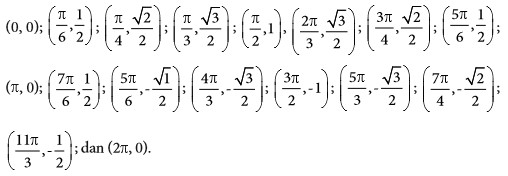
\includegraphics[scale=0.75]{fungsi_trigonometri_1}

Selanjutnya pada koordinat kartesius, kita menempatkan pasangan titiktitik untuk menemukan suatu kurva  yang melalui semua pasangan titik-titik tersebut. Selengkapnya disajikan pada Gambar berikut ini.\\

\begin{figure}[!ht]
\begin{center}
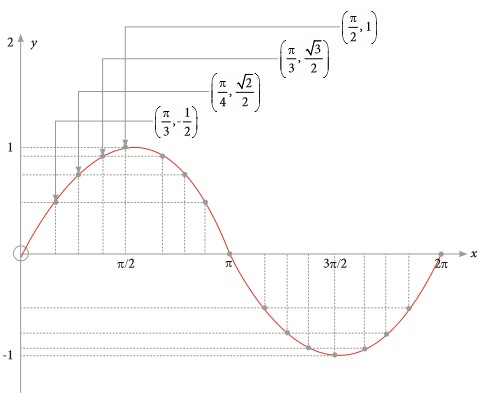
\includegraphics[scale=0.75]{grafik_fungsi_trigonometri_1}
\caption{Grafik fungsi $y = \sin x$, untuk $0 \leq x\leq 2\pi$}
\end{center}
\end{figure}

Dari grafik di atas,  kita dapat merangkum beberapa data dan informasi seperti berikut.
\begin{itemize}
\item Untuk semua ukuran sudut $x$,  nilai maksimum fungsi $y = \sin x$ adalah 1, dan nilai minimumnya adalah -1.
\item Kurva fungsi $y = \sin x$, berupa gelombang.
\item Untuk 1 periode (1 putaran penuh) kurva fungsi $y = \sin x$, memiliki 1 gunung dan 1 lembah.
\item Nilai fungsi sinus berulang saat berada pada lembah atau gunung yang sama.
\item Untuk semua ukuran sudut $x$, daerah hasil fungsi $y = \sin x$, adalah $1 \leq y \leq 1$. Dengan konsep grafik fungsi $y = \sin x$, dapat dibentuk kombinasi fungsi sinus.
\end{itemize}

Misalnya $y = 2.\sin x$, $y = \sin 2x$, dan $y = \sin (x+\pi/2)$ . Selengkapnya dikaji pada contoh berikut.

\begin{example}
Gambarkan grafik fungsi $y = \sin 2x$ dan $y = \sin (x+\pi/2)$, untuk $0 \leq x\leq 2\pi$. Kemudian tuliskanlah perbedaan kedua grafik tersebut.\\

\textbf{Alternatif Penyelesaian}\\
Dengan menggunakan nilai-nilai perbandingan trigonometri yang disajikan pada Tabel 4.3, maka pasangan titik-titik untuk fungsi $y = \sin 2x$, untuk $0 \leq x\leq 2\pi$ adalah:\\
Untuk $x = 0$, maka nilai fungsi adalah $y = \sin 2.(0) = \sin 0 = 0 \Rightarrow (0, 0)$\\
Untuk $x = (\pi/6)$, maka nilai fungsi adalah $y = \sin 2. (\pi/6) = \sin \pi/3 = \sqrt{3}/2 \Rightarrow(\pi/6,\sqrt{3}/2)$\\
Untuk $x = \pi/4$, maka nilai fungsi adalah $y = \sin 2. (\pi/4) = \sin \pi/2 = 1 \Rightarrow(\pi/4,1)$.\\
Demikian seterusnya hingga\\
untuk $x = 2\pi$, maka niali fungsi adalah $y = \sin 2.(2\pi) = \sin 4\pi = \sin 0 = 0 \Rightarrow (2\pi, 0)$\\
Selengkapnya pasangan titik-titik untuk fungsi $y = \sin 2x$, $0 \leq x\leq 2\pi$, yaitu

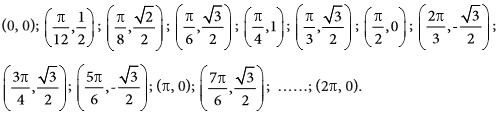
\includegraphics[scale=0.75]{fungsi_trigonometri_2}

Dengan  pasangan titik-titik tersebut, maka grafik fungsi $y = \sin 2x$, $0 \leq x\leq 2\pi$ disajikan pada Gambar.\\

\begin{figure}[!ht]
\begin{center}
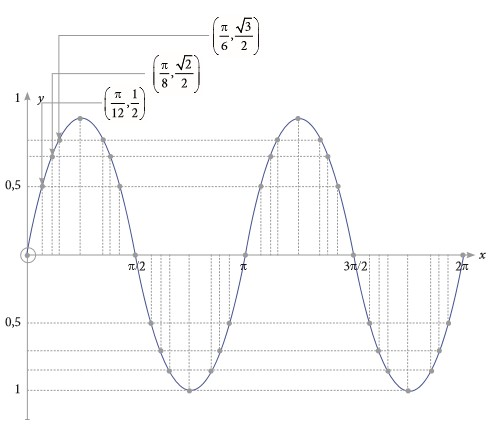
\includegraphics[scale=0.75]{grafik_fungsi_trigonometri_2} 
\caption{Grafik fungsi $y = \sin 2x$, untuk $0 \leq x\leq 2\pi$}
\end{center}
\end{figure}

Berbeda dengan fungsi $y = \sin 2x$, setiap besar sudut dikalikan dua, tetapi untuk fungsi $y = \sin(x+\pi/2)$, setiap besar sudut ditambah $\pi/2$ atau $90^o$.\\
Sekarang kita akan menggambarkan fungsi $y = \sin(x+\pi/2)$, untuk $0 \leq x\leq 2\pi$.\\
Coba kita perhatikan kembali, bahwa $\sin(x+\pi/2) = \cos x$. Artinya, sekarang kita akan menggambarkan fungsi $y = \cos x$, untuk $0 \leq x\leq 2\pi$. Dengan menggunakan nilai-nilai cosinus yang diberikan pada Tabel kita dapat merangkumkan pasangan titik-titik  yang memenuhi fungsi $y = \cos x$, untuk $0 \leq x\leq 2\pi$, sebagai berikut.

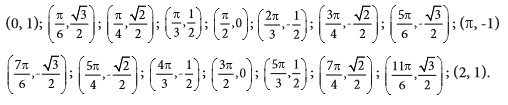
\includegraphics[scale=0.75]{fungsi_trigonometri_3}

Dengan demikian, grafik fungsi $y = \cos x$, untuk $0 \leq x\leq 2\pi$, disajikan pada Gambar berikut.\\

\begin{figure}[!ht]
\begin{center}
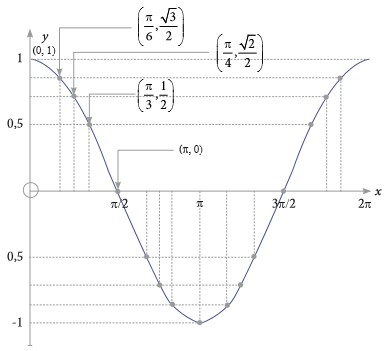
\includegraphics[scale=0.75]{grafik_fungsi_trigonometri_3} 
\caption{Grafik fungsi $y = \cos x$, untuk $0 \leq x\leq 2\pi$}
\end{center}
\end{figure}

Dari kajian grafik, grafik fungsi $y = \sin 2x$ sangat berbeda dengan grafik fungsi $y = \sin (x+\pi/2)  = \cos x$, meskipun untuk domain yang sama. Grafik $y = \sin 2x$, memiliki 2 gunung dan 2 lembah, sedangkan grafik fungsi $y = \sin (x+\pi/2)= \cos x$, hanya memiliki 1 lembah dan dua bagian setengah gunung. Nilai maksimum dan minimum fungsi $y = \sin 2x$ sama $y = \sin (x+\pi/2) = \cos x$ untuk domain yang sama. Selain itu, secara periodik, nilai fungsi $y = \sin 2x$ dan $y = \sin (x+\pi/2) = \cos x$, berulang, terkadang menaik dan terkadang menurun.
\end{example}
\begin{exercise}
Dengan pengetahuan dan keterampilan kamu akan tiga grafik di atas dan konsep yang sudah kamu miliki pada kajian fungsi, sekarang gambarkan dan gabungkan grafik $y = \sin x$ dan $y = \cos x$, untuk domain $0 \leq x\leq 2\pi$.\\
Rangkumkan hasil analisis yang kamu temukan atas grafik tersebut.
\end{exercise}
\item \textbf{Grafik Fungsi $y = tan x$, dan $y = \cos x$ untuk $0 \leq x\leq 2\pi$}\\
Kajian kita selanjutnya adalah untuk  menggambarkan grafik fungsi $y = \tan x$, untuk $0 \leq x\leq 2\pi$. Mari kita kaji grafik fungsi $y = \tan x$, melalui masalah berikut\\
\begin{problem}
Untuk domain $0 \leq x\leq 2\pi$, gambarkan grafik fungsi $y = \tan x$.\\
\end{problem}
\textbf{Alternatif Penyelesaian}\\
Dengan nilai-nilai tangen yang telah kita temukan pada Tabel 4.3 dan dengan pengetahuan serta keterampilan yang telah kamu pelajari tentang menggambarkan grafik suatu fungsi, kita dengan mudah memahami pasangan titik-titik berikut.\\

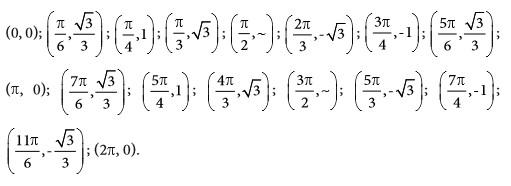
\includegraphics[scale=0.75]{fungsi_trigonometri_4}

Dengan demikian, grafik fungsi $y = \tan x$, untuk $0 \leq x\leq 2\pi$, seperti pada Gambar berikut ini.\\

\begin{figure}[!ht]
\begin{center}
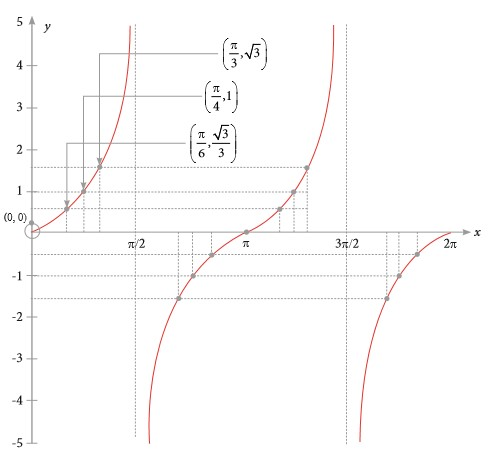
\includegraphics[scale=0.75]{grafik_fungsi_trigonometri_4} 
\caption{Grafik fungsi $y = \tan x$, untuk $0 \leq x\leq 2\pi$}
\end{center}
\end{figure}

Dari grafik di atas, jelas kita lihat bahwa jika $x$ semakin mendekati $\pi/2$ (dari kiri), nilai fungsi semakin besar, tetapi tidak dapat ditentukan nilai terbesarnya. Sebaliknya, jika $x$ atau mendekati $\pi/2$ (dari kanan), maka nilai fungsi semakin kecil, tetapi tidak dapat ditentukan nilai terkecilnya. Kondisi ini berulang pada saat $x$ mendekati $3\pi/2$. Artinya, fungsi $y = \tan x$, tidak memiliki nilai maksimum dan minimum.
\end{enumerate}
%------------------------------------------------
%----------------------------------------------------------------------------------------
%	BIBLIOGRAPHY
%----------------------------------------------------------------------------------------

\chapter*{Bibliography}
\addcontentsline{toc}{chapter}{\textcolor{ocre}{Bibliography}}
\section*{Books}
\addcontentsline{toc}{section}{Books}
\printbibliography[heading=bibempty,type=book]
\section*{Articles}
\addcontentsline{toc}{section}{Articles}
\printbibliography[heading=bibempty,type=article]

%----------------------------------------------------------------------------------------
%	INDEX
%----------------------------------------------------------------------------------------

\cleardoublepage
\phantomsection
\setlength{\columnsep}{0.75cm}
\addcontentsline{toc}{chapter}{\textcolor{ocre}{Index}}
\printindex

%----------------------------------------------------------------------------------------

\end{document}
